\documentclass[12pt,a4paper]{report}
\usepackage[utf8]{inputenc}
\usepackage[T1]{fontenc}
\usepackage[margin=1in]{geometry}
\usepackage{amsmath,amssymb}
\usepackage{graphicx}
\usepackage{booktabs}
\usepackage{array}
\usepackage{tabularx}
\usepackage{xcolor}
\usepackage{url}
\usepackage{setspace}
\usepackage{cite}
\usepackage{tikz}
\usetikzlibrary{arrows.meta,positioning,shapes.geometric,fit}
\usepackage{pgfplots}
\pgfplotsset{compat=1.17}
\usepackage[hidelinks]{hyperref}

\onehalfspacing
\renewcommand{\bibname}{Bibliography}

\tikzset{
  blk/.style={draw, rounded corners=3pt, align=center, inner sep=5pt, font=\small},
  arr/.style={-{Stealth[length=2.2mm]}, thick},
  darr/.style={{Stealth[length=2.2mm]}-{Stealth[length=2.2mm]}, thick}
}

\begin{document}

%======================== TITLE PAGE ========================
\begin{titlepage}
\centering
\vspace*{1.2cm}
{\LARGE\bfseries MentorConnect: An Evidence-Driven Platform for\\[4pt] Institutional Peer Mentoring and Mentor Recommendation\par}
\vspace{1.4cm}
{\large submitted in partial fulfillment of the requirement\\ for the award of the Degree of\par}
\vspace{1.2cm}
{\large\bfseries Bachelor of Technology\par}
{\large in\par}
{\large\bfseries Computer Engineering\par}
\vspace{1.2cm}
{\large by\par}
\vspace{0.6cm}
{\large\bfseries Himani Arvind Pilankar (2024301021)\\ Tithi Kiran Talele (2024301034)\\ Chetan Vijay Wankhede (2024301035)\par}
\vspace{1.2cm}
{\large under the guidance of\par}
\vspace{0.4cm}
{\large\bfseries Dr. Sudhir Dhage\par}
\vfill
{\large\bfseries Department of Computer Engineering\par}
{\large Bharatiya Vidya Bhavan's\\ Sardar Patel Institute of Technology\\ (Autonomous Institute Affiliated to University of Mumbai)\\ Munshi Nagar, Andheri-West, Mumbai-400058\\ University of Mumbai\\ November 2026\par}
\end{titlepage}

%======================== CERTIFICATE ========================
\thispagestyle{empty}
\begin{center}
\vspace*{1cm}
{\Large\bfseries Certificate\par}
\end{center}
\vspace{1cm}
\noindent This is to certify that the Project entitled ``MentorConnect: An Evidence-Driven Platform for Institutional Peer Mentoring and Mentor Recommendation'' has been completed to our satisfaction by Ms.\ Himani Arvind Pilankar, Ms.\ Tithi Kiran Talele and Mr.\ Chetan Vijay Wankhede under the guidance of Dr.\ Sudhir Dhage for the award of Degree of Bachelor of Technology in Computer Engineering from University of Mumbai.

\vspace{2cm}
\begin{center}{\bfseries Certified by}\end{center}
\vspace{2cm}
\noindent\begin{tabular}{@{}p{0.5\textwidth}@{}p{0.5\textwidth}@{}}
\textbf{Dr. Sudhir Dhage} & \hfill\textbf{Head of Department}\\
\textbf{Project Guide} & \hfill\textbf{Computer Engineering}
\end{tabular}

\vspace{2.5cm}
\begin{center}
\textbf{Principal}\\
\textbf{Sardar Patel Institute of Technology}
\end{center}
\vfill
\begin{center}
{\bfseries Department of Computer Engineering}\\
Bharatiya Vidya Bhavan's\\ Sardar Patel Institute of Technology\\ (Autonomous Institute Affiliated to University of Mumbai)\\ Munshi Nagar, Andheri(W), Mumbai-400058\\ University of Mumbai\\ November 2026
\end{center}
\clearpage

%======================== APPROVAL CERTIFICATE ========================
\thispagestyle{empty}
\begin{center}
\vspace*{1cm}
{\Large\bfseries Project Approval Certificate\par}
\end{center}
\vspace{1.5cm}
\noindent This is to certify that the Project entitled ``MentorConnect: An Evidence-Driven Platform for Institutional Peer Mentoring and Mentor Recommendation'' by Ms.\ Himani Arvind Pilankar, Ms.\ Tithi Kiran Talele and Mr.\ Chetan Vijay Wankhede is found to be satisfactory and is approved for the award of Degree of Bachelor of Technology in Computer Engineering from University of Mumbai.

\vspace{4cm}
\noindent\begin{tabular}{@{}p{0.5\textwidth}@{}p{0.5\textwidth}@{}}
\textbf{External Examiner} & \hfill\textbf{Internal Examiner}\\[2.5cm]
\textbf{(signature)} & \hfill\textbf{(signature)}\\[0.8cm]
\textbf{Name:} & \hfill\textbf{Name:}\qquad\qquad\qquad\\[1cm]
\textbf{Date:} & \hfill\textbf{Date:}\qquad\qquad\qquad\;
\end{tabular}

\vfill
\begin{center}\textbf{Seal of the Institute}\end{center}
\vspace{2cm}
\clearpage

%======================== STATEMENT ========================
\thispagestyle{empty}
\begin{center}
\vspace*{1cm}
{\Large\bfseries Statement by the Candidates\par}
\end{center}
\vspace{1.5cm}
\noindent We wish to state that the work embodied in this thesis titled ``MentorConnect: An Evidence-Driven Platform for Institutional Peer Mentoring and Mentor Recommendation'' forms our own contribution to the work carried out under the guidance of Dr.\ Sudhir Dhage at the Sardar Patel Institute of Technology. We declare that this written submission represents our ideas in our own words and where others' ideas or words have been included, we have adequately cited and referenced the original sources. We also declare that we have adhered to all principles of academic honesty and integrity and have not misrepresented or fabricated or falsified any idea/data/fact/source in our submission.

\vspace{6cm}
\noindent\textbf{Name and Signature:}\\
\textbf{1. Himani Arvind Pilankar}\\
\textbf{2. Tithi Kiran Talele}\\
\textbf{3. Chetan Vijay Wankhede}
\clearpage

%======================== ACKNOWLEDGMENTS ========================
\chapter*{Acknowledgments}
\thispagestyle{empty}
It is a pleasure to acknowledge the help and support that went into making this thesis. We express our sincere gratitude to our guide, Dr.\ Sudhir Dhage, for his invaluable guidance throughout the project. His encouragement to treat a practical platform as a subject of careful research shaped the direction of this work, and the freedom he gave us made working under him a genuinely rewarding experience.

We thank the Head of Department and the Department of Computer Engineering for providing the facilities and support required to carry out this work, and the students who shared their experiences of seeking and giving mentorship, which helped us understand the problem we set out to solve.

Finally, we thank our families and well-wishers for their constant encouragement over these years, without which we could not have completed this work.

%======================== FRONT MATTER ========================
\pagenumbering{roman}
\tableofcontents
\listoffigures
\listoftables

\chapter*{Abstract}
\addcontentsline{toc}{chapter}{Abstract}
Peer mentoring helps students succeed, yet in most institutes it still happens through personal networks and messaging groups, so students without a network struggle to find the right senior, helpful mentors go unrecognised, and the institute cannot see what students need. This project presents MentorConnect, an institute-only web platform that formalises peer mentoring: verified sign-up with institute email, structured academic profiles, mentorship requests, real-time chat, communities, a mentor recommendation engine, session tracking, and verifiable achievement certificates.

The central idea of the project is \emph{evidence gating}. A mentor's track record is the most useful signal for recommending them, but it is also the easiest to fake, because in mentoring the mentor usually records the activity. In MentorConnect, a mentoring session counts only after the mentee confirms it and supplies the feedback; confirmed records are locked, and a mentee can report that a session never happened. Only these verified records feed the recommendation engine and the certificate system. The engine is a hybrid ranker implemented as a separate Python service, combining skill coverage, TF-IDF profile similarity, project relevance and availability with shrunk, mentee-verified quality, activity and responsiveness signals, and returning an explanation for every ranked mentor. Every recommendation list is logged so that ranking quality can be measured from real use.

We evaluated the approach on simulated campuses with hidden ground truth and three manipulation strategies, using the platform's ranking code and 20 random seeds with paired significance tests. Trusting all logged activity lowered NDCG@10 from 0.716 to 0.630 and gave manipulators 32.9\% of top-10 slots against a 14.7\% share of the mentor pool. With the ranking model held fixed, the evidence gate raised NDCG@10 by 0.033 and top-5 precision by 0.071 and cut manipulator exposure from 26.4\% to 19.1\% in every run, and pushed self-logged inflators below random-chance exposure. Compared with ranking on profiles alone, verified history improved top-5 precision by 7\%, rising to 17\% as history accumulated, and counting at most one session per mentee further reduced colluder exposure by 22\% while improving every accuracy metric. The project shows that a practical mentoring platform can be both useful to students and resistant to the gaming that undermines reputation-based recommendation.

\clearpage
\pagenumbering{arabic}

%======================== CHAPTER 1 ========================
\chapter{Introduction}
Peer mentoring is one of the most valuable forms of support in higher education. Senior students guide juniors on subjects, projects, internships and career choices, and research on student retention shows that this kind of social and academic integration helps students persist \cite{tinto1993}. In most engineering institutes, however, mentoring is informal. It happens in personal chats, messaging groups and chance conversations. These channels have no structure or continuity and leave no record.

Informal mentoring creates three problems. First, access is unequal: students who are hesitant or lack a peer network find it hard to approach the right senior, so the students who most need guidance often receive the least. Second, impact is invisible: mentors who help many juniors receive no formal recognition, and the institute cannot see which topics students struggle with or which mentors make a difference. Third, mentoring programmes rarely capture structured outcome data, which makes them hard to evaluate or improve \cite{gershenfeld2014}.

A digital platform can address all three problems by giving students a verified place to find mentors, request mentorship and record sessions. Doing this well, however, raises a harder question. A recommender that ranks mentors by their track record must trust the records it is given, and in mentoring the person being ranked is usually the one who logs the activity. A mentor who records sessions that never happened, rates them highly, or asks friends to vouch for them can climb the rankings and draw attention away from genuinely helpful peers. This is a people-matching version of the profile-injection attacks studied in recommender systems \cite{lam2004,mobasher2007} and of the inflation problems in online reputation systems \cite{resnick2000,josang2007}.

MentorConnect is our answer to both needs. It is an institute-only mentoring platform built around one principle, \emph{evidence gating}: a mentor's history can influence their ranking and their recognition only through records that the mentee created and verified.

\section{Problem Statement}
In most engineering institutes, student mentoring takes place through unstructured channels that lack verification, structure, continuity and analytical visibility. There is no centralised system that helps students find a suitable mentor, captures mentoring interactions as trustworthy structured data, or recognises mentors for the help they actually provide. Where mentor history is used to recommend mentors, it can be inflated by the mentors themselves. The problem is to design and build a verified institutional mentoring platform whose mentor recommendations and recognition rest on evidence that mentees have confirmed, and to evaluate whether this makes recommendation both accurate and resistant to manipulation.

\section{Objectives}
The key objectives of the project are as follows:
\begin{itemize}
\item To provide a verified, institute-exclusive platform where students can create academic profiles, discover mentors and manage mentorships from request to completion.
\item To recommend mentors to each student using a hybrid, explainable ranking that combines topical fit with the mentor's verified track record.
\item To capture mentoring sessions as structured data in which ratings, outcomes and follow-ups are supplied only by the mentee, and to lock confirmed records against later edits.
\item To recognise mentors through auditable contribution points, achievement levels and publicly verifiable certificates based only on verified sessions.
\item To log every recommendation list and the actions that follow it, so that ranking quality can be measured from real use.
\item To evaluate experimentally whether evidence gating makes mentor recommendation resistant to manipulation without reducing accuracy.
\end{itemize}

\section{Scope}
MentorConnect covers institute-only registration with OTP verification; role-based access for juniors, seniors and administrators; academic profiles; mentor discovery and recommendation; the mentorship lifecycle; mentoring session logging, confirmation and dispute; real-time chat and notifications; communities, groups, posts and subject-tagged discussions; topic-based Tech Circles; achievements and certificates; and a consent-controlled External Guidance mode through which learners from outside the institute can seek help from mentors who have opted in. The recommendation engine and its evaluation form the research component of the project.

\section{Layout of the Report}
A brief overview of each chapter is provided here.\\
Chapter 2: A survey of research on mentoring, learning analytics, recommender systems and reputation systems, together with a review of existing mentoring platforms.\\
Chapter 3: The design of MentorConnect, including its architecture, modules, evidence-gated session verification and recommendation engine.\\
Chapter 4: Results, covering system verification, an audit of the original recommendation engine, and the manipulation experiment.\\
Chapter 5: Conclusions and future work.\\
Chapter 6: The research paper prepared from this work.

%======================== CHAPTER 2 ========================
\chapter{Literature Survey}
\section{Mentoring and Learning Analytics}
``Leaving College: Rethinking the Causes and Cures of Student Attrition'' \cite{tinto1993} by Vincent Tinto is a foundational account of why students leave higher education. Tinto argues that persistence depends on a student's academic and social integration into the institution, and that relationships with peers and seniors are a central part of that integration. The work establishes why structured peer support matters, but it is a theoretical account and does not propose a mechanism for building such support at scale.

``A Review of Undergraduate Mentoring Programs'' \cite{gershenfeld2014} by Susan Gershenfeld reviews a large body of research on undergraduate mentoring programmes. It finds wide variation in how programmes are designed and observes that many evaluations are methodologically weak, with little structured data on what mentoring actually achieves. This gap motivates MentorConnect's emphasis on capturing every mentoring session as structured, verified data.

``Penetrating the Fog: Analytics in Learning and Education'' \cite{siemens2011} by George Siemens and Phil Long describes how data on learner activity can inform teaching and institutional decisions, and introduces learning analytics as a field. ``Learning Analytics: Drivers, Developments and Challenges'' \cite{ferguson2012} by Rebecca Ferguson traces the forces behind the field and highlights challenges of data quality, ethics and meaningful use. Both works show the value of structured activity data; neither addresses mentoring, which in most institutes is not recorded at all. ``Privacy and Analytics: It's a DELICATE Issue'' \cite{drachsler2016} by Hendrik Drachsler and Wolfgang Greller proposes a checklist for trustworthy learning analytics, stressing consent, transparency and legitimate purpose. MentorConnect follows these principles in its consent-based External Guidance mode and its private profile fields.

\section{Recommender Systems}
``Recommender Systems'' \cite{resnick1997} by Paul Resnick and Hal Varian introduced the idea of systems that aggregate people's signals to suggest items. ``Hybrid Recommender Systems: Survey and Experiments'' \cite{burke2002} by Robin Burke surveys ways of combining content-based and collaborative methods so that the strengths of each compensate for the weaknesses of the other, particularly when data are sparse. ``Collaborative Filtering Recommender Systems'' \cite{ekstrand2011} by Ekstrand, Riedl and Konstan explains how collaborative filtering learns from dense interaction histories, an assumption that does not hold for campus mentoring, where most mentors have only a handful of sessions. MentorConnect therefore uses a hybrid design in which content similarity, computed with TF-IDF weighting \cite{salton1988}, carries most of the weight and behavioural evidence is added with statistical shrinkage.

``RECON: A Reciprocal Recommender for Online Dating'' \cite{pizzato2010} by Pizzato et al.\ shows that recommending people differs from recommending items: a match succeeds only if both sides are willing. MentorConnect includes this reciprocal view through a mentor responsiveness signal, the smoothed share of requests a mentor accepts. ``Controlling Popularity Bias in Learning-to-Rank Recommendation'' \cite{abdollahpouri2017} by Abdollahpouri, Burke and Mobasher shows that rankers that reward accumulated activity concentrate exposure on popular items. In mentoring this would overload a few seniors and hide capable newcomers, so we measure newcomer exposure and exposure concentration in our evaluation.

\section{Manipulation and Reputation}
``Shilling Recommender Systems for Fun and Profit'' \cite{lam2004} by Lam and Riedl demonstrated that injecting fake profiles and ratings can push chosen items up a recommender's rankings. ``Toward Trustworthy Recommender Systems: An Analysis of Attack Models and Algorithm Robustness'' \cite{mobasher2007} by Mobasher et al.\ formalised these attack models and measured how robust different algorithms are, and ``Shilling Attacks against Recommender Systems: A Comprehensive Survey'' \cite{gunes2014} by Gunes et al.\ surveys attacks and the detection methods proposed against them. Most of these defences detect suspicious profiles after the fact. In mentoring the attacker is the item being recommended, which suggests a different defence: controlling who is allowed to create evidence in the first place.

``Reputation Systems'' \cite{resnick2000} by Resnick et al.\ explains how aggregated feedback builds trust between strangers, and ``A Survey of Trust and Reputation Systems for Online Service Provision'' \cite{josang2007} by J{\o}sang, Ismail and Boyd reviews the models used in practice and their weaknesses. ``Can Online Reviews Reveal a Product's True Quality?'' \cite{hu2006} by Hu, Pavlou and Zhang shows that self-selection gives online ratings a J-shaped distribution, so averages can mislead. ``The Sybil Attack'' \cite{douceur2002} by Douceur shows that a system without identity verification cannot prevent one party from posing as many. MentorConnect's institute-verified accounts limit Sybil attacks, and its mentee-only feedback addresses self-reported inflation; collusion between real students remains possible and is measured in Chapter~4.

\section{Review of Existing Mentoring Platforms}
Table~\ref{tab:platforms} summarises the options available to students today. None of them combines institute-verified identity, structured peer mentoring and verified evidence of real help.

\begin{table}[h]
\centering
\caption{Existing mentoring platforms and their limits in a campus setting}
\label{tab:platforms}
\small
\begin{tabularx}{\textwidth}{>{\raggedright\arraybackslash}p{3.4cm}XX}
\toprule
\textbf{Platform} & \textbf{What it provides} & \textbf{Limits in a campus setting}\\
\midrule
Messaging groups and personal chats & Fast, familiar and free communication & No discovery, no records, no recognition\\
LinkedIn & Professional profiles and messaging & Not institute-verified; no mentoring workflow\\
ADPList & Open mentor directory with session booking & Global and external; not tied to the institute\\
MentorCruise, Topmate & Paid one-to-one mentoring sessions & Paid; not designed for peer mentoring\\
Enterprise mentoring software & Programme management and matching & Licensed products; little peer-level verification\\
\bottomrule
\end{tabularx}
\end{table}

\section{Research Gap}
\begin{table}[h]
\centering
\caption{Summary of the research gap}
\label{tab:gap}
\small
\begin{tabularx}{\textwidth}{>{\raggedright\arraybackslash}p{3.4cm}XX}
\toprule
\textbf{Area} & \textbf{What existing work provides} & \textbf{Key gap}\\
\midrule
Mentoring research & Evidence that peer support helps students & No structured capture of mentoring\\
Recommender systems & Hybrid and collaborative methods & Sparse, two-sided people matching\\
Learning analytics & Turning activity data into insight & Activity is not proof of real help\\
Reputation systems & Trust from aggregated feedback & Ratees often record their own activity\\
Existing platforms & Directories, chats, paid sessions & No institute-verified peer mentoring\\
\bottomrule
\end{tabularx}
\end{table}

Existing work shows that peer mentoring matters, that structured data enables better decisions, and that reputation signals can be gamed. What is missing is an institutional mentoring platform that ranks and recognises mentors using evidence the mentees themselves verified. MentorConnect is designed to fill this gap.

%======================== CHAPTER 3 ========================
\chapter{MentorConnect System}
\section{Architecture}
\begin{figure}[h]
\centering
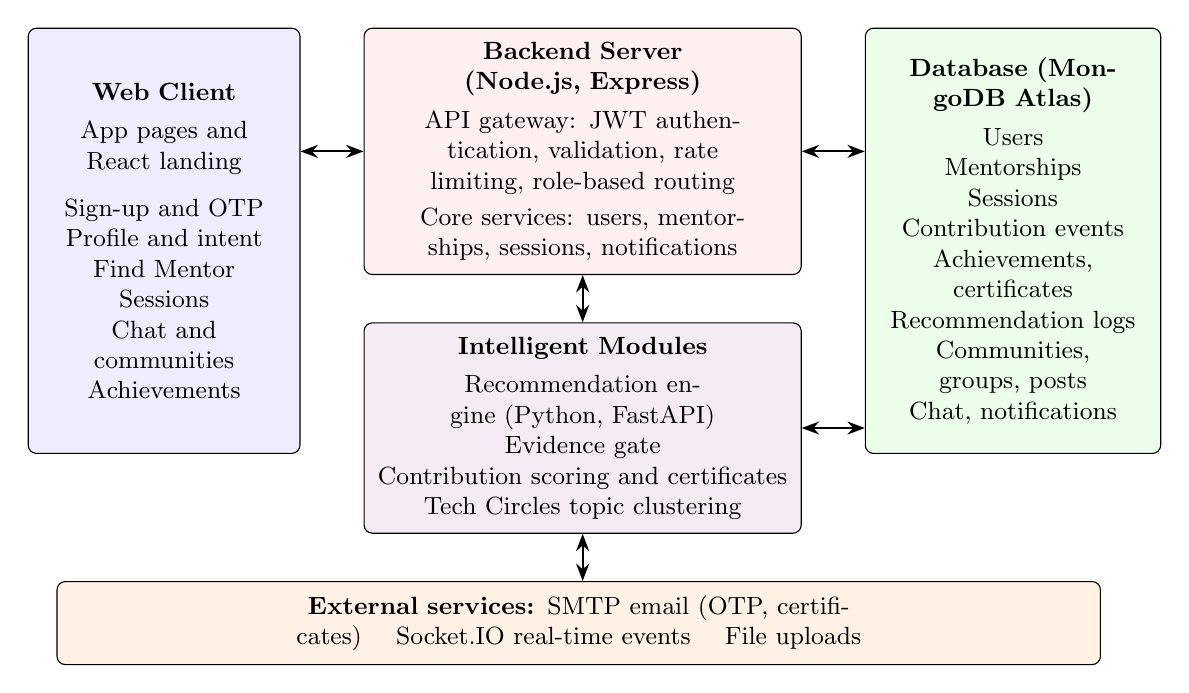
\begin{tikzpicture}[node distance=6mm and 6mm]
\node[blk, fill=blue!7, text width=3.1cm, minimum height=5.4cm] (client) {\textbf{Web Client}\\[3pt] App pages and React landing\\[6pt] Sign-up and OTP\\ Profile and intent\\ Find Mentor\\ Sessions\\ Chat and communities\\ Achievements};
\node[blk, fill=red!6, text width=5.2cm, right=8mm of client.north east, anchor=north west, minimum height=2.5cm] (backend) {\textbf{Backend Server (Node.js, Express)}\\[3pt] API gateway: JWT authentication, validation, rate limiting, role-based routing\\[2pt] Core services: users, mentorships, sessions, notifications};
\node[blk, fill=violet!8, text width=5.2cm, below=6mm of backend, minimum height=2.5cm] (mods) {\textbf{Intelligent Modules}\\[3pt] Recommendation engine (Python, FastAPI)\\ Evidence gate\\ Contribution scoring and certificates\\ Tech Circles topic clustering};
\node[blk, fill=green!8, text width=3.4cm, right=8mm of backend.north east, anchor=north west, minimum height=5.4cm] (db) {\textbf{Database (MongoDB Atlas)}\\[3pt] Users\\ Mentorships\\ Sessions\\ Contribution events\\ Achievements, certificates\\ Recommendation logs\\ Communities, groups, posts\\ Chat, notifications};
\node[blk, fill=orange!10, text width=12.9cm, below=6mm of mods.south west, anchor=north west, xshift=-3.9cm] (ext) {\textbf{External services:} SMTP email (OTP, certificates) \quad Socket.IO real-time events \quad File uploads};
\draw[darr] (client.east |- backend.west) -- (backend.west);
\draw[darr] (backend) -- (mods);
\draw[darr] (backend.east) -- (db.west |- backend.east);
\draw[darr] (mods.east) -- (db.west |- mods.east);
\draw[darr] (mods.south) -- (mods.south |- ext.north);
\end{tikzpicture}
\caption{System architecture of MentorConnect}
\label{fig:arch}
\end{figure}

Figure~\ref{fig:arch} shows the architecture of MentorConnect. Students use a set of browser pages served by the backend, together with a React and Vite landing page. All requests pass through an Express API gateway that verifies JSON Web Tokens, validates and sanitises input, applies rate limits and enforces role-based permissions. Core services manage users, mentorships, sessions and notifications, and Socket.IO delivers chat messages, typing indicators, online status and notifications in real time.

The intelligent modules sit behind the backend. The recommendation engine runs as a separate Python FastAPI service, which lets the project evolve and evaluate ranking models independently of the web application; if the service is unavailable, the backend falls back to a built-in JavaScript engine. The evidence gate controls which session records count as evidence, the contribution service converts verified sessions into points, achievement levels and certificates, and the Tech Circles module groups students by shared technical interests. All data is stored in MongoDB Atlas through Mongoose schemas with indexes for the main query patterns.

\section{User Roles and Workflow}
\begin{table}[h]
\centering
\caption{User roles in MentorConnect}
\label{tab:roles}
\small
\begin{tabularx}{\textwidth}{>{\raggedright\arraybackslash}p{3.2cm}X}
\toprule
\textbf{Role} & \textbf{Main capabilities}\\
\midrule
Student (junior or senior) & Build a profile, find and request mentors, offer mentoring, log and confirm sessions, chat, join communities and groups\\
Administrator & Manage the platform, configure the academic year, review consent summaries\\
External learner & Seek mentorship from institute mentors who have opted in; browse approved communities\\
\bottomrule
\end{tabularx}
\end{table}

Any student who chooses ``offering'' or ``both'' as their mentorship intent can mentor any other student. There is no seniority constraint, so peers in the same year can help each other, and a junior with the right skills can mentor a senior. Figure~\ref{fig:flow} shows the end-to-end workflow.

\begin{figure}[h]
\centering
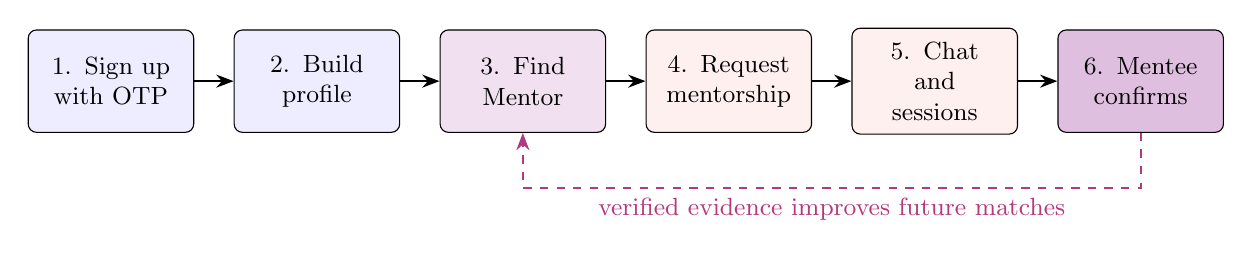
\begin{tikzpicture}[node distance=5mm]
\node[blk, fill=blue!7, text width=1.75cm, minimum height=1.3cm] (s1) {1. Sign up\\ with OTP};
\node[blk, fill=blue!7, text width=1.75cm, minimum height=1.3cm, right=of s1] (s2) {2. Build\\ profile};
\node[blk, fill=violet!12, text width=1.75cm, minimum height=1.3cm, right=of s2] (s3) {3. Find\\ Mentor};
\node[blk, fill=red!6, text width=1.75cm, minimum height=1.3cm, right=of s3] (s4) {4. Request\\ mentorship};
\node[blk, fill=red!6, text width=1.75cm, minimum height=1.3cm, right=of s4] (s5) {5. Chat and\\ sessions};
\node[blk, fill=violet!25, text width=1.75cm, minimum height=1.3cm, right=of s5] (s6) {6. Mentee\\ confirms};
\draw[arr] (s1) -- (s2);
\draw[arr] (s2) -- (s3);
\draw[arr] (s3) -- (s4);
\draw[arr] (s4) -- (s5);
\draw[arr] (s5) -- (s6);
\draw[arr, dashed, magenta!70!black] (s6.south) -- ++(0,-0.7) -| node[pos=0.25, below, font=\small]{verified evidence improves future matches} (s3.south);
\end{tikzpicture}
\caption{End-to-end workflow of MentorConnect}
\label{fig:flow}
\end{figure}

\section{System Modules}
\subsection{Authentication and Identity}
Registration is restricted to institute email domains and verified with a one-time password sent by email. Passwords are hashed with bcrypt, and a successful login returns a seven-day JSON Web Token. Each account carries a role (junior, senior or administrator) and an identity type (institute member or external learner), and every protected route checks both.

\subsection{Profiles}
A profile holds the student's department, year, skills, interests, projects, bio, availability and mentorship intent. Sensitive admission details are stored in fields that are never returned in public profile responses. A profile-strength indicator encourages students to complete their profiles, which improves the quality of recommendations.

\subsection{Mentorship Lifecycle}
A student sends a mentorship request with a short reason. The mentor can accept or decline it; accepting opens a private chat group for the pair, and either side can later end the mentorship. Duplicate active or pending requests are prevented, and each step generates a notification. Figure~\ref{fig:lifecycle} shows the states of a mentorship and of a mentoring session.

\begin{figure}[h]
\centering
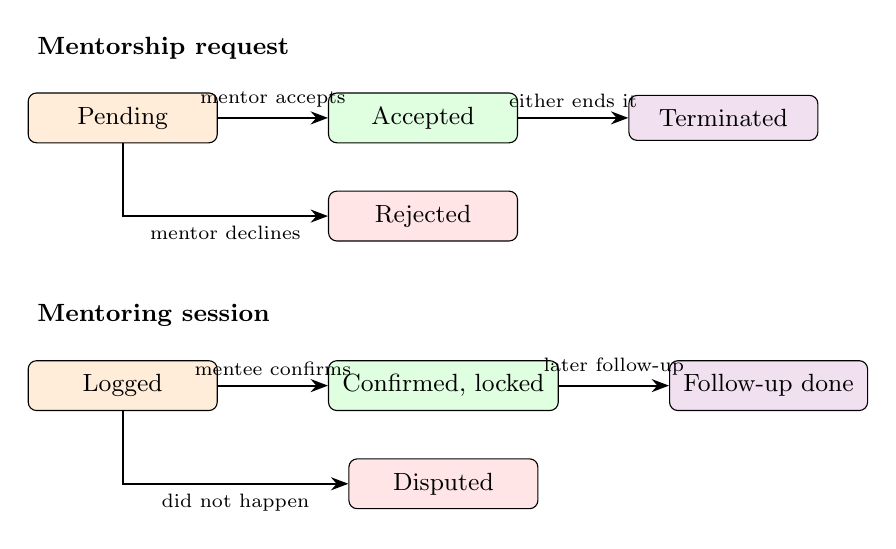
\begin{tikzpicture}[node distance=6mm and 14mm]
\node[font=\small\bfseries, anchor=west] (t1) at (0,0) {Mentorship request};
\node[blk, fill=orange!15, minimum width=2.4cm, below=3mm of t1.south west, anchor=north west] (p) {Pending};
\node[blk, fill=green!12, minimum width=2.4cm, right=of p] (a) {Accepted};
\node[blk, fill=violet!12, minimum width=2.4cm, right=of a] (t) {Terminated};
\node[blk, fill=red!10, minimum width=2.4cm, below=of a] (r) {Rejected};
\draw[arr] (p) -- node[above, font=\scriptsize]{mentor accepts} (a);
\draw[arr] (a) -- node[above, font=\scriptsize]{either ends it} (t);
\draw[arr] (p) |- node[pos=0.75, below, font=\scriptsize]{mentor declines} (r);
\node[font=\small\bfseries, anchor=west] (t2) at (0,-3.4) {Mentoring session};
\node[blk, fill=orange!15, minimum width=2.4cm, below=3mm of t2.south west, anchor=north west] (l) {Logged};
\node[blk, fill=green!12, minimum width=2.4cm, right=of l] (c) {Confirmed, locked};
\node[blk, fill=violet!12, minimum width=2.4cm, right=of c] (f) {Follow-up done};
\node[blk, fill=red!10, minimum width=2.4cm, below=of c] (d) {Disputed};
\draw[arr] (l) -- node[above, font=\scriptsize]{mentee confirms} (c);
\draw[arr] (c) -- node[above, font=\scriptsize]{later follow-up} (f);
\draw[arr] (l) |- node[pos=0.75, below, font=\scriptsize]{did not happen} (d);
\end{tikzpicture}
\caption{Lifecycle of a mentorship request and of a mentoring session}
\label{fig:lifecycle}
\end{figure}

\subsection{Sessions and the Evidence Gate}\label{sec:gate}
The Sessions page is where mentoring is recorded. A mentor logs a session with its topic, subject, type and duration, and the mentee is notified. The mentee then confirms the session and gives the feedback: a star rating, whether the problem was solved, whether the agreed follow-up happened, and whether they would recommend the mentor. If the session never took place, the mentee can dispute it instead. A mentee may also log a session they received, in which case it is confirmed at once with their feedback. The rules that make this evidence trustworthy are enforced on the server:
\begin{itemize}
\item Ratings, outcomes and recommendations can be written only by the mentee; anything a mentor submits in these fields is discarded.
\item A confirmed session is locked. The only permitted change is that the mentee may later record that a follow-up was completed.
\item A disputed session is excluded permanently, and the mentor is notified.
\item A confirmation counts as evidence only if the mentee is an email-verified current student of the institute. Sessions confirmed by external or alumni accounts are kept in the history but do not affect rankings, points or certificates, so a mentor cannot create outside accounts to vouch for themselves.
\end{itemize}
Figure~\ref{fig:gate} shows the verification flow, and Algorithm~1 summarises it.

\begin{figure}[h]
\centering
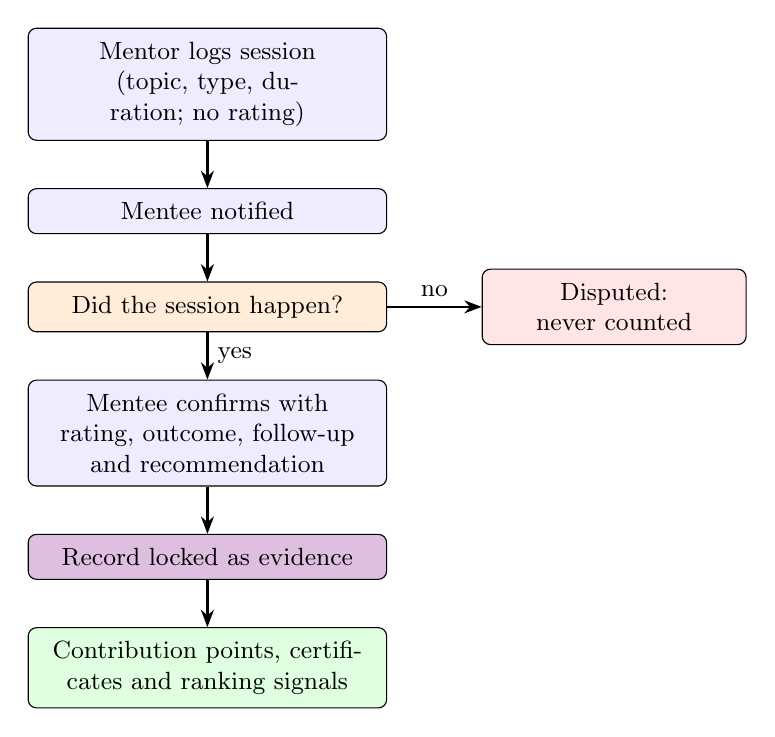
\begin{tikzpicture}[node distance=6mm]
\node[blk, fill=blue!7, text width=4.2cm] (m) {Mentor logs session\\ (topic, type, duration; no rating)};
\node[blk, fill=blue!7, text width=4.2cm, below=of m] (n) {Mentee notified};
\node[blk, fill=orange!15, text width=4.2cm, below=of n] (q) {Did the session happen?};
\node[blk, fill=blue!7, text width=4.2cm, below=of q] (c) {Mentee confirms with rating, outcome, follow-up and recommendation};
\node[blk, fill=violet!25, text width=4.2cm, below=of c] (lk) {Record locked as evidence};
\node[blk, fill=green!12, text width=4.2cm, below=of lk] (o) {Contribution points, certificates and ranking signals};
\node[blk, fill=red!10, text width=3cm, right=12mm of q] (d) {Disputed:\\ never counted};
\draw[arr] (m) -- (n);
\draw[arr] (n) -- (q);
\draw[arr] (q) -- node[right, font=\small]{yes} (c);
\draw[arr] (q) -- node[above, font=\small]{no} (d);
\draw[arr] (c) -- (lk);
\draw[arr] (lk) -- (o);
\end{tikzpicture}
\caption{Evidence-gated session verification}
\label{fig:gate}
\end{figure}

\noindent\textbf{Algorithm 1: Evidence-gated session verification}\\
\textbf{Input:} a logged session $s$. \textbf{Output:} locked evidence, or a disputed record.
\begin{enumerate}
\item Record the topic, subject, type and duration logged by the mentor.
\item Discard any rating, outcome or recommendation sent by the mentor.
\item Mark $s$ as pending and notify the mentee.
\item If the mentee reports that $s$ did not happen, mark it disputed, notify the mentor and stop.
\item Store the mentee's rating, outcome, follow-up and recommendation, and mark $s$ confirmed.
\item Count $s$ as evidence only if the mentee is a verified current student of the institute.
\item Lock $s$ against further edits.
\item Award contribution points once per event type.
\item Update the mentor's quality, activity and recency signals.
\end{enumerate}

\subsection{Achievements and Certificates}
Each confirmed session produces auditable contribution events: verified activity, quality feedback, a resolved outcome, a completed follow-up and a new mentee, each awarded at most once per session. Five achievement levels require minimum numbers of sessions, distinct mentees and resolved outcomes together with a minimum average rating, so a certificate cannot be earned through volume alone. Earned certificates are emailed to the mentor, shown on their profile and can be verified publicly by certificate ID.

\subsection{Collaboration Features}
MentorConnect includes a feed of posts with comments and likes, subject-tagged discussions with voting and resolved status, interest communities with membership rules, groups with roles, real-time chat and notifications. Tech Circles groups students into topic clusters based on their skills and interests, helping them find peers who share their technical interests.

\subsection{External Guidance}
Mentors may opt in to guiding learners from outside the institute. Opting in requires accepting a versioned set of terms, and the choice is locked until the end of the academic year so that external learners are not left without support. External learners can only seek mentorship, see only mentors who have opted in, and cannot use features such as private messaging or groups.

\section{Recommendation Engine}
\begin{figure}[h]
\centering
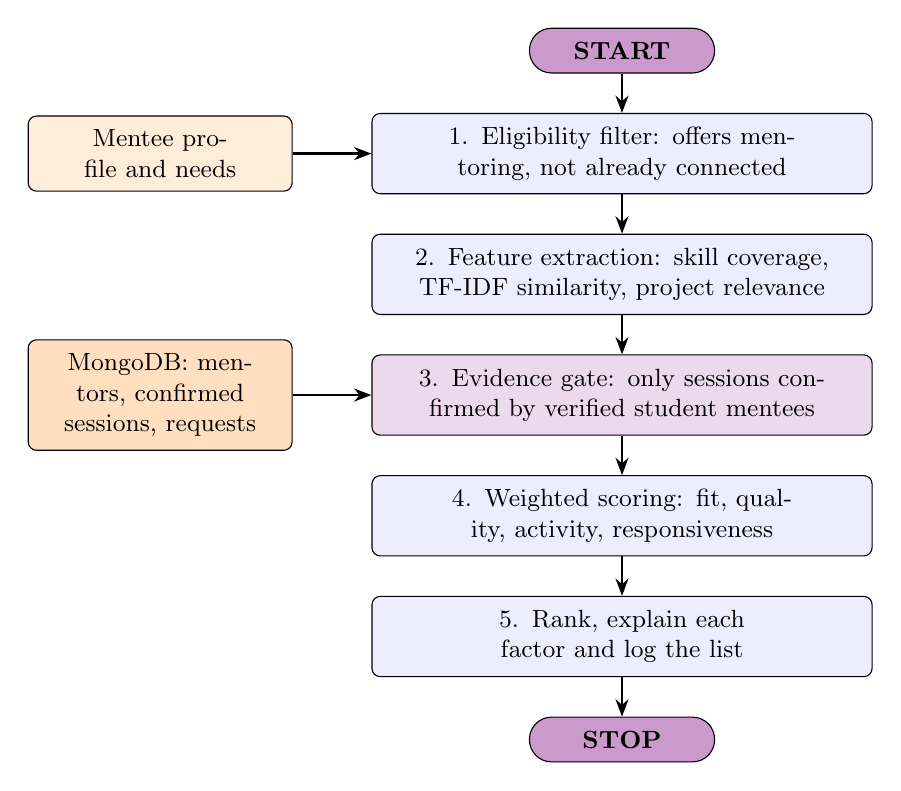
\begin{tikzpicture}[node distance=5mm]
\node[blk, fill=violet!40, rounded corners=8pt, text width=2cm] (st) {\textbf{START}};
\node[blk, fill=blue!7, text width=6cm, below=of st] (b1) {1. Eligibility filter: offers mentoring, not already connected};
\node[blk, fill=blue!7, text width=6cm, below=of b1] (b2) {2. Feature extraction: skill coverage, TF-IDF similarity, project relevance};
\node[blk, fill=violet!15, text width=6cm, below=of b2] (b3) {3. Evidence gate: only sessions confirmed by verified student mentees};
\node[blk, fill=blue!7, text width=6cm, below=of b3] (b4) {4. Weighted scoring: fit, quality, activity, responsiveness};
\node[blk, fill=blue!7, text width=6cm, below=of b4] (b5) {5. Rank, explain each factor and log the list};
\node[blk, fill=violet!40, rounded corners=8pt, text width=2cm, below=of b5] (sp) {\textbf{STOP}};
\node[blk, fill=orange!15, text width=3cm, left=10mm of b1] (in) {Mentee profile and needs};
\node[blk, fill=orange!25, text width=3cm, left=10mm of b3] (dbn) {MongoDB: mentors, confirmed sessions, requests};
\draw[arr] (st) -- (b1);
\draw[arr] (b1) -- (b2);
\draw[arr] (b2) -- (b3);
\draw[arr] (b3) -- (b4);
\draw[arr] (b4) -- (b5);
\draw[arr] (b5) -- (sp);
\draw[arr] (in) -- (b1);
\draw[arr] (dbn) -- (b3);
\end{tikzpicture}
\caption{Recommendation engine pipeline}
\label{fig:engine}
\end{figure}

Figure~\ref{fig:engine} shows how the engine ranks mentors for a student. It first keeps only eligible mentors: those who offer mentoring and are not already in an active or pending mentorship with the student. External learners see only mentors who have opted in to External Guidance. The engine then computes fit features: the share of the student's needs covered by the mentor's skills and interests, TF-IDF cosine similarity between profile texts \cite{salton1988}, the relevance of the mentor's projects, and department, year and availability matches. A seeded K-Means step groups similar mentors and contributes a small cluster-fit term.

\subsection{Verified Evidence Signals}
Let $G_m$ be the set of confirmed sessions for mentor $m$. With $n$ ratings averaging $\bar\rho$ in $G_m$, the rating is pulled toward a neutral prior $\mu_0 = 3.5$ with strength $k = 5$ and weighted by its confidence:
\begin{equation}
\tilde\rho = \frac{k\mu_0 + n\bar\rho}{k+n}, \qquad c = \frac{n}{n+k}.
\end{equation}
Mentor quality combines the rating with the completion rate $\kappa$, the share of confirmed sessions that were resolved or followed up, and the smoothed ``would recommend'' rate $\omega$:
\begin{equation}
Q_m = 0.8\left(0.6\,c\,\frac{\tilde\rho}{5} + 0.4\,\kappa\right) + 0.2\,\omega .
\end{equation}
Activity combines volume and recency, $A_m = 0.5\min(1, |G_m|/60) + 0.5\max(0, 1 - \Delta t/90)$, where $\Delta t$ is the number of days since the last confirmed session. Responsiveness is the share of requests the mentor accepted, smoothed with a Beta(2,2) prior so that a new mentor starts at 0.5 rather than 0.

\subsection{Scoring and Explanation}
The final score of mentor $m$ for student $s$ is a weighted sum of the fit and evidence features,
\begin{equation}
S(s,m) = \sum_{k} w_k\, f_k(s,m), \qquad \sum_k w_k = 1 .
\end{equation}
Table~\ref{tab:weights} lists the weights of the original engine (V1) and of the evidence-gated engine (V3). Every recommendation is returned with the contribution of each factor, so a student can see why a mentor was suggested.

\begin{table}[h]
\centering
\caption{Scoring weights of the original (V1) and evidence-gated (V3) engines}
\label{tab:weights}
\small
\begin{tabular}{lrr@{\hspace{1.2cm}}lrr}
\toprule
\textbf{Fit factor} & \textbf{V1} & \textbf{V3} & \textbf{Evidence factor} & \textbf{V1} & \textbf{V3}\\
\midrule
Skill coverage & 0.20 & 15.0\% & Mentor quality & 0.18 & 13.5\%\\
Profile text (TF-IDF) & 0.12 & 9.0\% & Activity and recency & 0.11 & 8.3\%\\
Project relevance & -- & 7.5\% & Verified mentoring evidence & -- & 6.0\%\\
Same department & 0.10 & 7.5\% & Responsiveness & -- & 3.8\%\\
Year gap & 0.10 & 7.5\% & Topic overlap & -- & 3.8\%\\
Availability & 0.08 & 6.0\% & Cluster fit and bonus & 0.08 & 6.1\%\\
Profile completeness & 0.08 & 6.0\% & & & \\
\bottomrule
\end{tabular}
\end{table}

The V1 weights sum to 1.05 and the score is clipped, and V1 counts every logged session whether or not it was confirmed. V3 normalises the weights, adds project relevance, verified mentoring evidence, responsiveness and topic overlap, and uses only confirmed sessions.

\subsection{Engine Versions}
The engine is developed as a sequence of versions that run on identical inputs, so each change can be measured against the original. Table~\ref{tab:versions} summarises them.

\begin{table}[h]
\centering
\caption{Recommendation engine versions}
\label{tab:versions}
\small
\begin{tabularx}{\textwidth}{>{\raggedright\arraybackslash}p{1.8cm}X>{\raggedright\arraybackslash}p{3.6cm}}
\toprule
\textbf{Version} & \textbf{Description} & \textbf{Status}\\
\midrule
V1 & Original engine, frozen with fixed random seeds as the research baseline & Built and audited\\
V2.0--V2.4 & Step-by-step variants: normalised weights, needs and offers, vocabulary, capacity, topic clustering & Built as selectable variants\\
V3 & Evidence-gated hybrid ranker with responsiveness and capacity awareness & Built; runs in the platform\\
V4 & Gradient-boosted (XGBoost) ranker over V3 features, explained with SHAP & Experimental\\
\bottomrule
\end{tabularx}
\end{table}

\subsection{Recommendation Logging}
Each time a student opens Find Mentor, the list shown is stored with every mentor's rank and score and the engine version. Later actions are attached to that list: viewing a mentor's details, opening their profile, marking a match as helpful or not, sending a request, and the mentor accepting or rejecting it. Requests, acceptances and rejections are recorded by the server itself, so they cannot be forged by the browser. These logs make it possible to compute online metrics such as request rate in the top five and top ten, mean reciprocal rank and acceptance rate for each engine version.

\section{Data Model}
\begin{figure}[h]
\centering
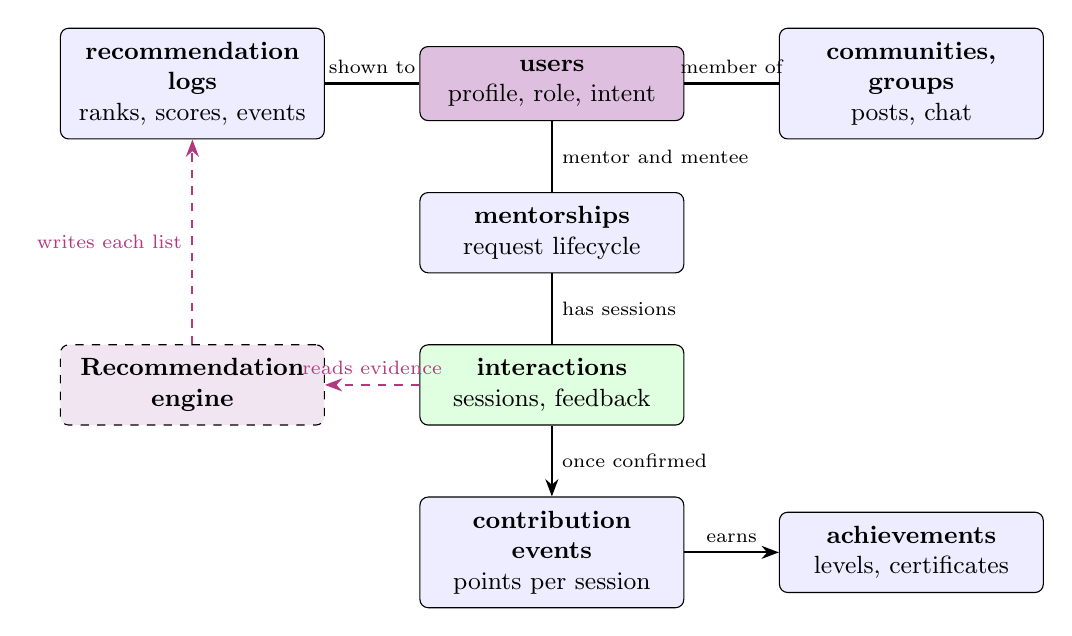
\begin{tikzpicture}[node distance=9mm and 12mm]
\node[blk, fill=violet!25, text width=3cm] (u) {\textbf{users}\\ profile, role, intent};
\node[blk, fill=blue!7, text width=3cm, left=of u] (rl) {\textbf{recommendation logs}\\ ranks, scores, events};
\node[blk, fill=blue!7, text width=3cm, right=of u] (cg) {\textbf{communities, groups}\\ posts, chat};
\node[blk, fill=blue!7, text width=3cm, below=of u] (ms) {\textbf{mentorships}\\ request lifecycle};
\node[blk, fill=green!12, text width=3cm, below=of ms] (it) {\textbf{interactions}\\ sessions, feedback};
\node[blk, fill=violet!10, dashed, text width=3cm, left=of it] (en) {\textbf{Recommendation engine}};
\node[blk, fill=blue!7, text width=3cm, below=of it] (ce) {\textbf{contribution events}\\ points per session};
\node[blk, fill=blue!7, text width=3cm, right=of ce] (ac) {\textbf{achievements}\\ levels, certificates};
\draw[thick] (rl) -- node[above, font=\scriptsize]{shown to} (u);
\draw[thick] (u) -- node[above, font=\scriptsize]{member of} (cg);
\draw[thick] (u) -- node[right, font=\scriptsize]{mentor and mentee} (ms);
\draw[thick] (ms) -- node[right, font=\scriptsize]{has sessions} (it);
\draw[arr] (it) -- node[right, font=\scriptsize]{once confirmed} (ce);
\draw[arr] (ce) -- node[above, font=\scriptsize]{earns} (ac);
\draw[arr, dashed, magenta!70!black] (it) -- node[above, font=\scriptsize]{reads evidence} (en);
\draw[arr, dashed, magenta!70!black] (en) -- node[left, font=\scriptsize]{writes each list} (rl);
\end{tikzpicture}
\caption{Main collections and their relationships}
\label{fig:data}
\end{figure}

Figure~\ref{fig:data} shows the main MongoDB collections. A mentorship links a mentor and a mentee; each mentorship has sessions; each confirmed session produces contribution events, which unlock achievement levels and certificates. The recommendation engine reads only confirmed evidence, and every list it produces is written to the recommendation logs. Demonstration data used for presentations is kept in a separate, clearly labelled collection and never mixes with real sessions.

\section{Security and Privacy}
MentorConnect follows the OWASP Top 10 guidance \cite{owasp2021}: passwords are hashed with bcrypt, sessions use signed JSON Web Tokens, security headers are set with Helmet, every API is rate-limited, and all input is validated and sanitised. Role and identity checks are enforced on the server for every protected route. On the privacy side, registration is limited to institute email domains, admission details are never exposed in public profiles, and External Guidance requires versioned, recorded consent \cite{drachsler2016}. The integrity rules of the evidence gate are part of this design, because the recommender and the certificate system both trust confirmed evidence.

\section{Technology Stack}
\begin{table}[h]
\centering
\caption{Technology stack}
\label{tab:stack}
\small
\begin{tabularx}{\textwidth}{>{\raggedright\arraybackslash}p{3.2cm}X}
\toprule
\textbf{Layer} & \textbf{Technologies}\\
\midrule
Frontend & HTML, CSS and JavaScript application pages; React 19 with Vite for the landing page\\
Backend & Node.js, Express, Socket.IO\\
Database & MongoDB Atlas, Mongoose\\
Recommendation & Python, FastAPI, scikit-learn, XGBoost, SHAP\\
Security & JSON Web Tokens, bcrypt, Helmet, express-rate-limit, express-validator\\
Services & Nodemailer (SMTP) for OTP and certificates, Multer for file uploads\\
\bottomrule
\end{tabularx}
\end{table}

%======================== CHAPTER 4 ========================
\chapter{Results and Analysis}
\section{Implementation and User Interface}
MentorConnect has been implemented in full and runs as a web application connected to a MongoDB Atlas database, with the recommendation engine served by its Python service. This section walks through every screen of the working application, captured while running the system and signing in as a student.

\subsection{Public Pages}
\begin{figure}[htbp]
\centering
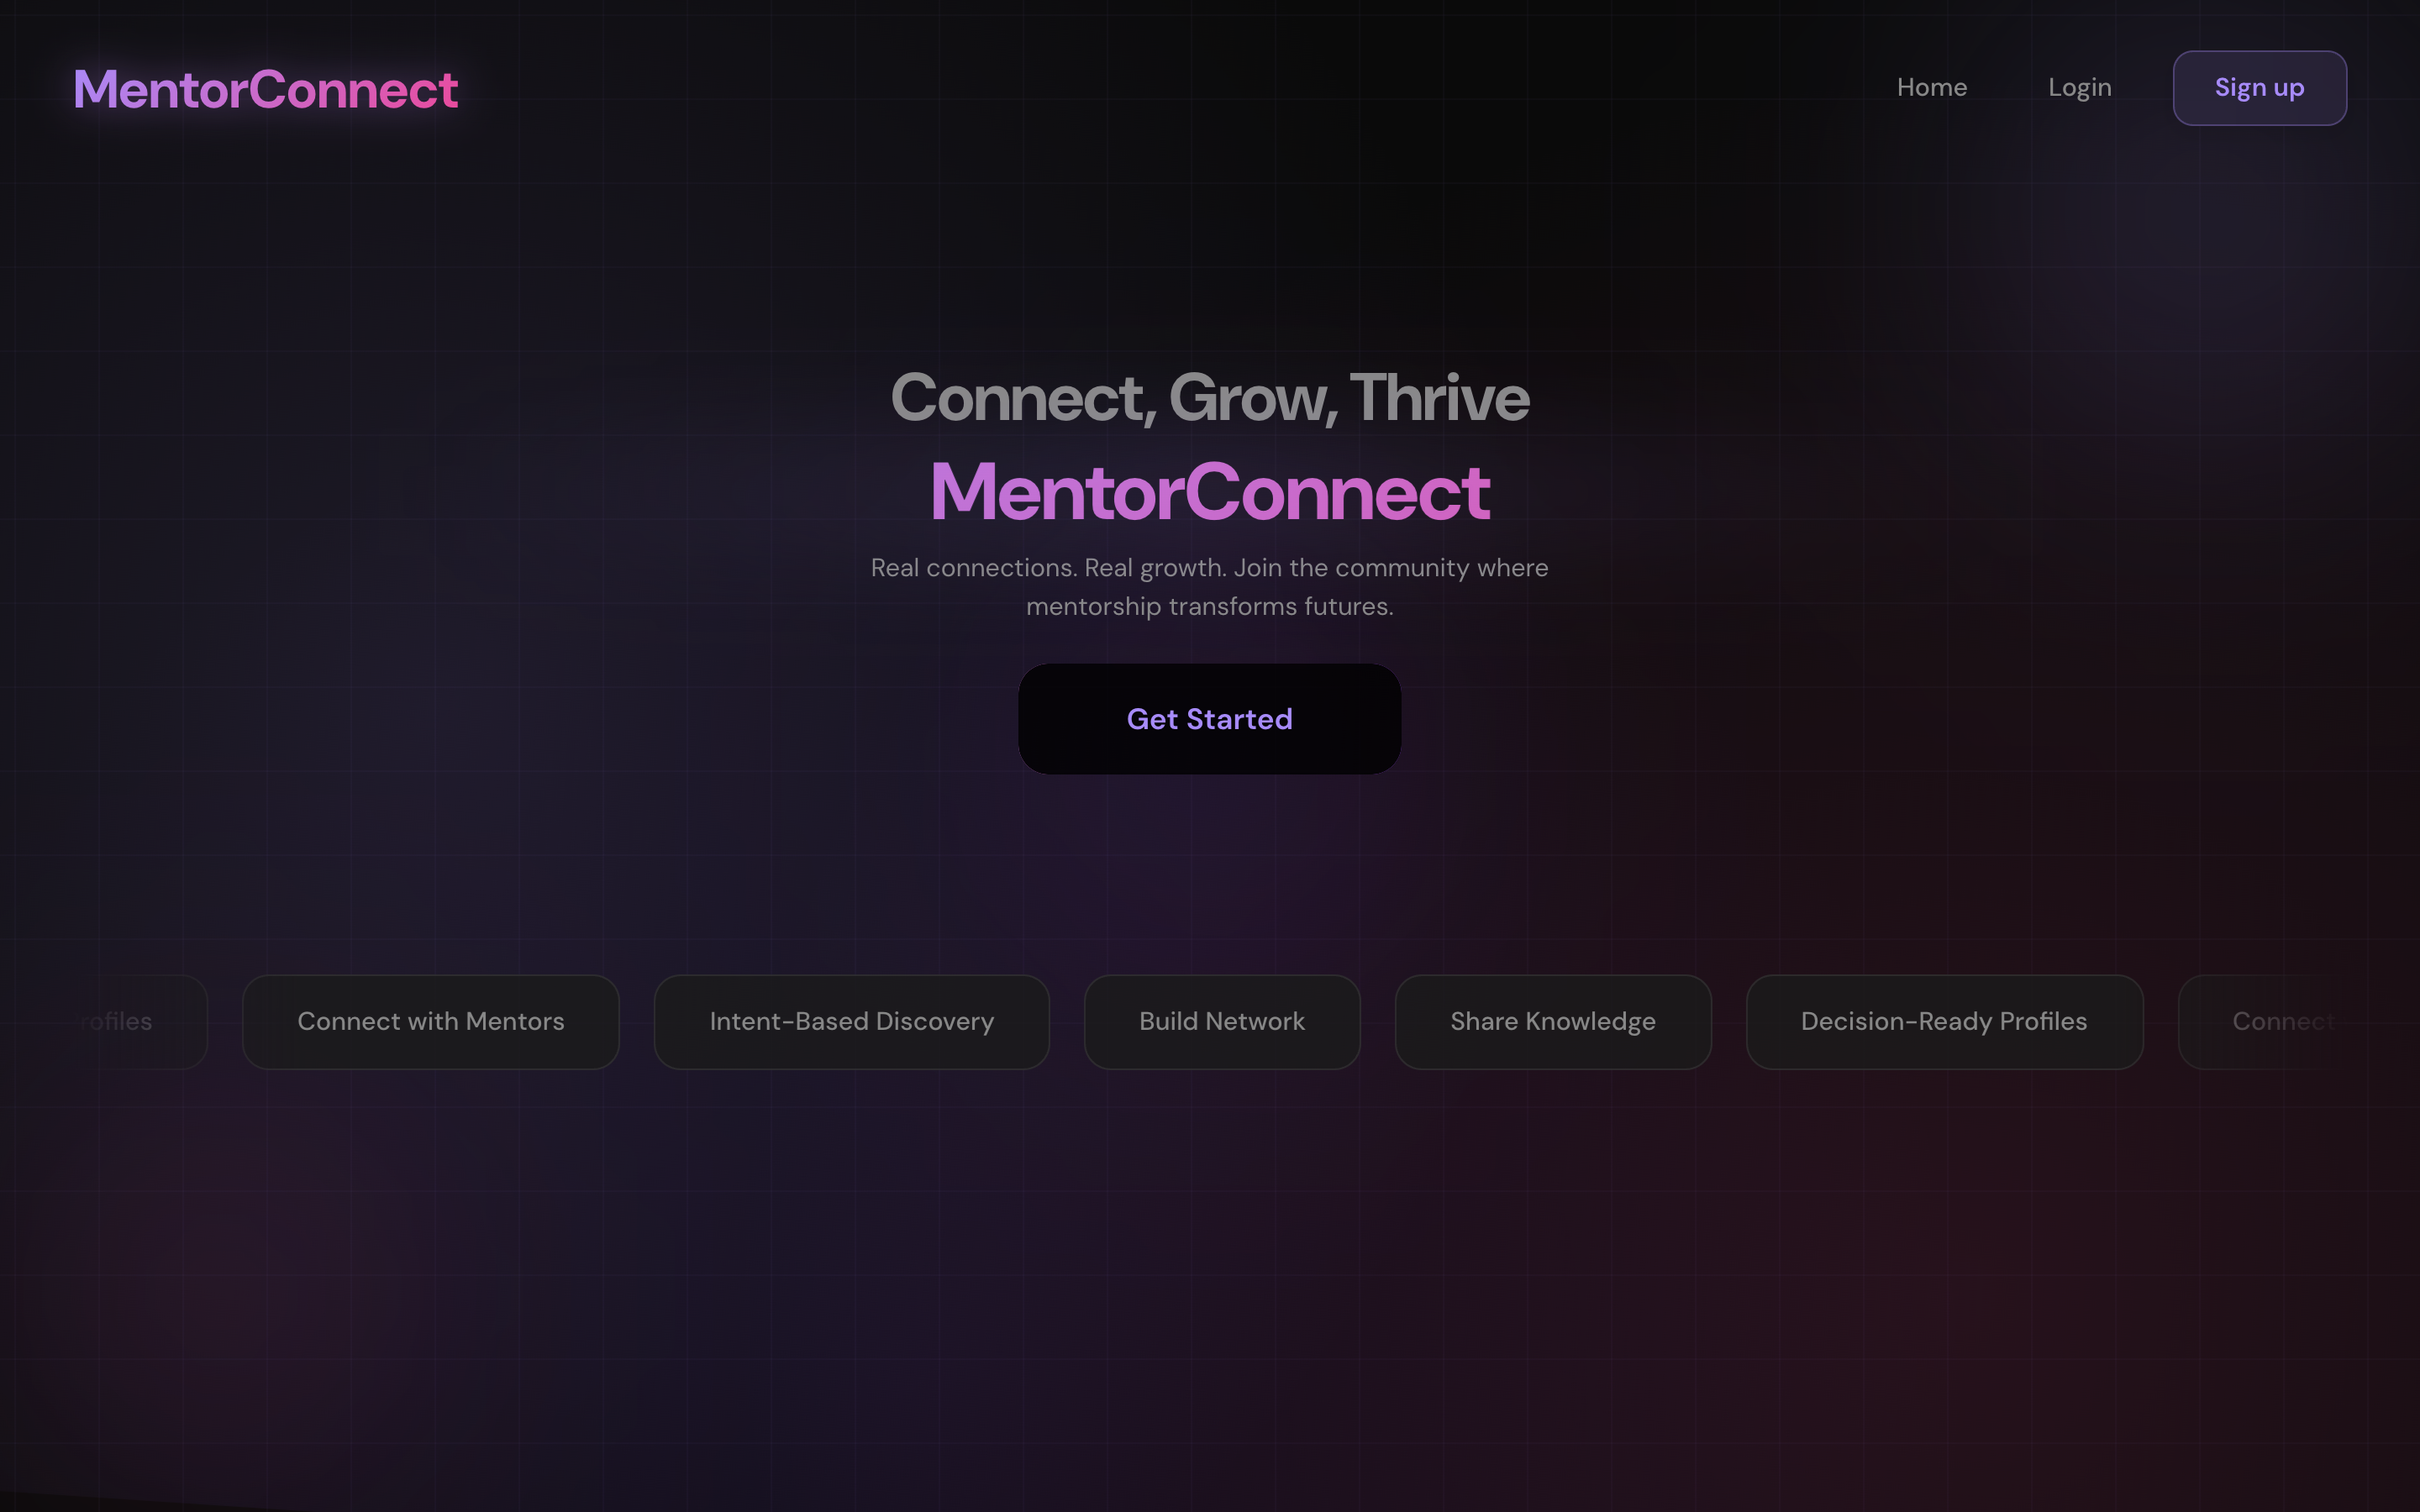
\includegraphics[width=0.95\textwidth]{figures/landing.png}
\caption{Landing page of MentorConnect}
\label{fig:ui-landing}
\end{figure}

\begin{figure}[htbp]
\centering
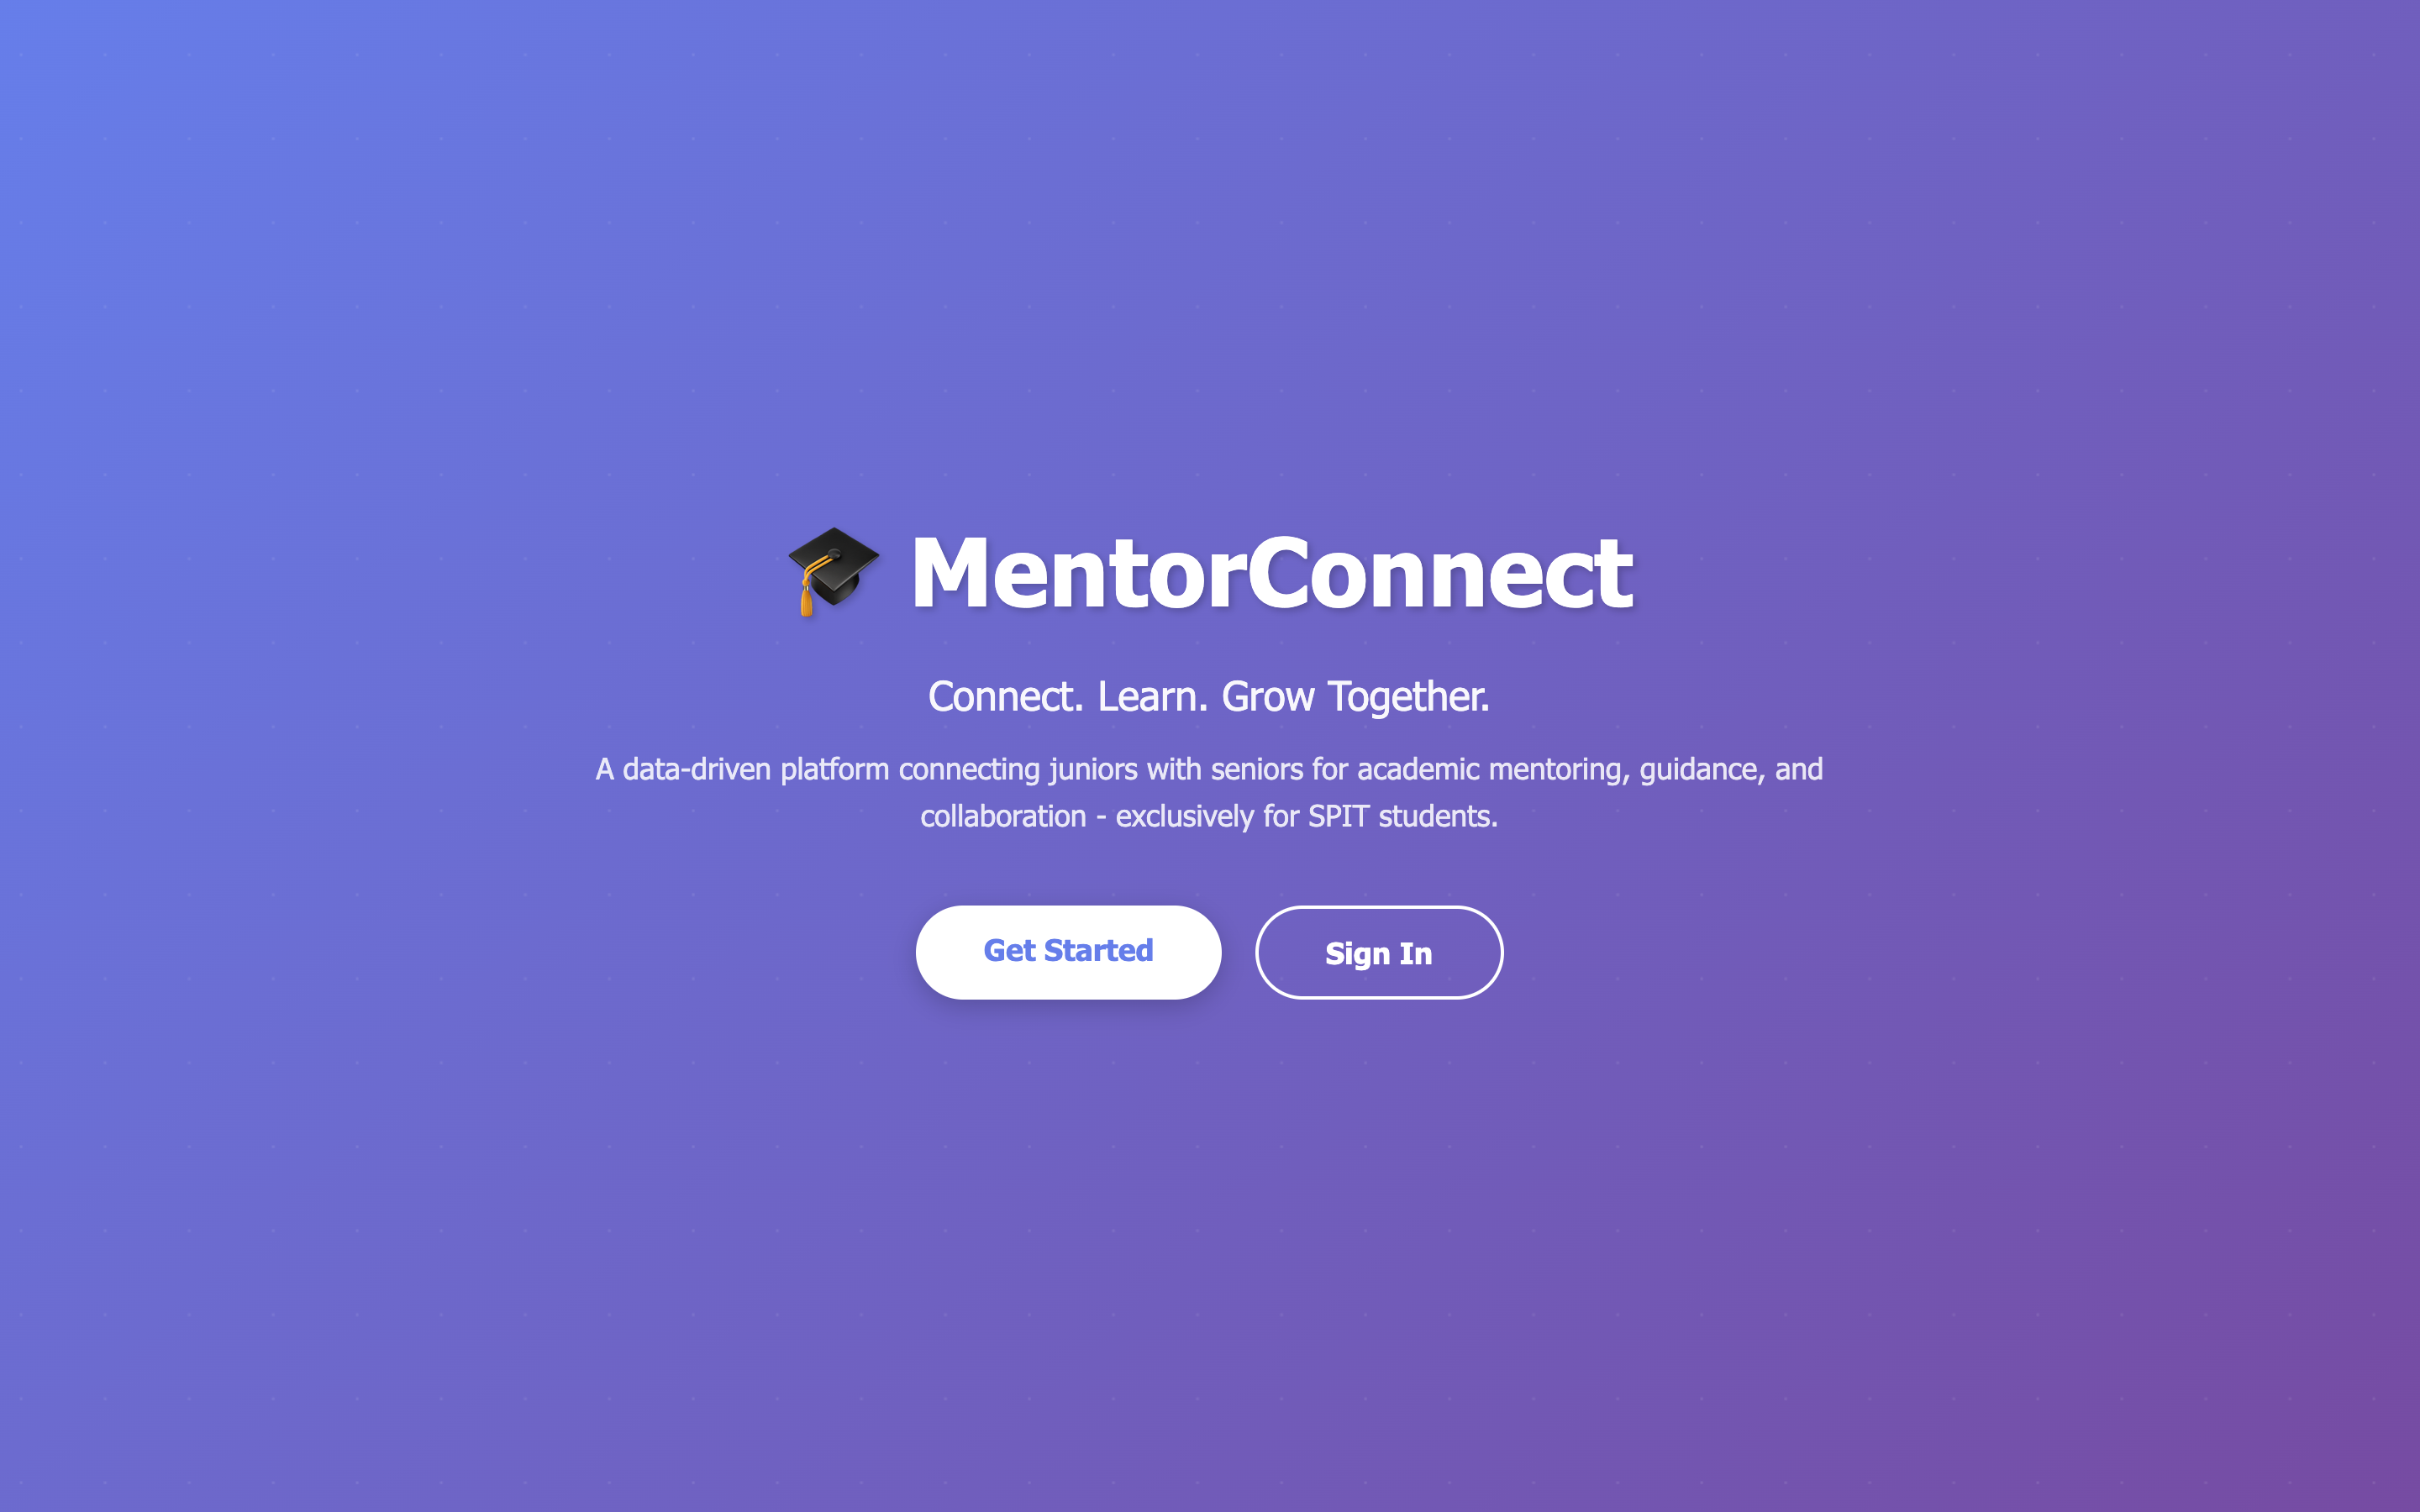
\includegraphics[width=0.95\textwidth]{figures/landing-page.png}
\caption{Welcome page served by the platform with sign-up and sign-in actions}
\label{fig:ui-welcome}
\end{figure}

The landing page (Figure~\ref{fig:ui-landing}) introduces the platform and its main ideas: connecting with mentors, intent-based discovery, building a network and sharing knowledge. The welcome page served by the backend (Figure~\ref{fig:ui-welcome}) leads students to sign up or sign in.

\begin{figure}[htbp]
\centering
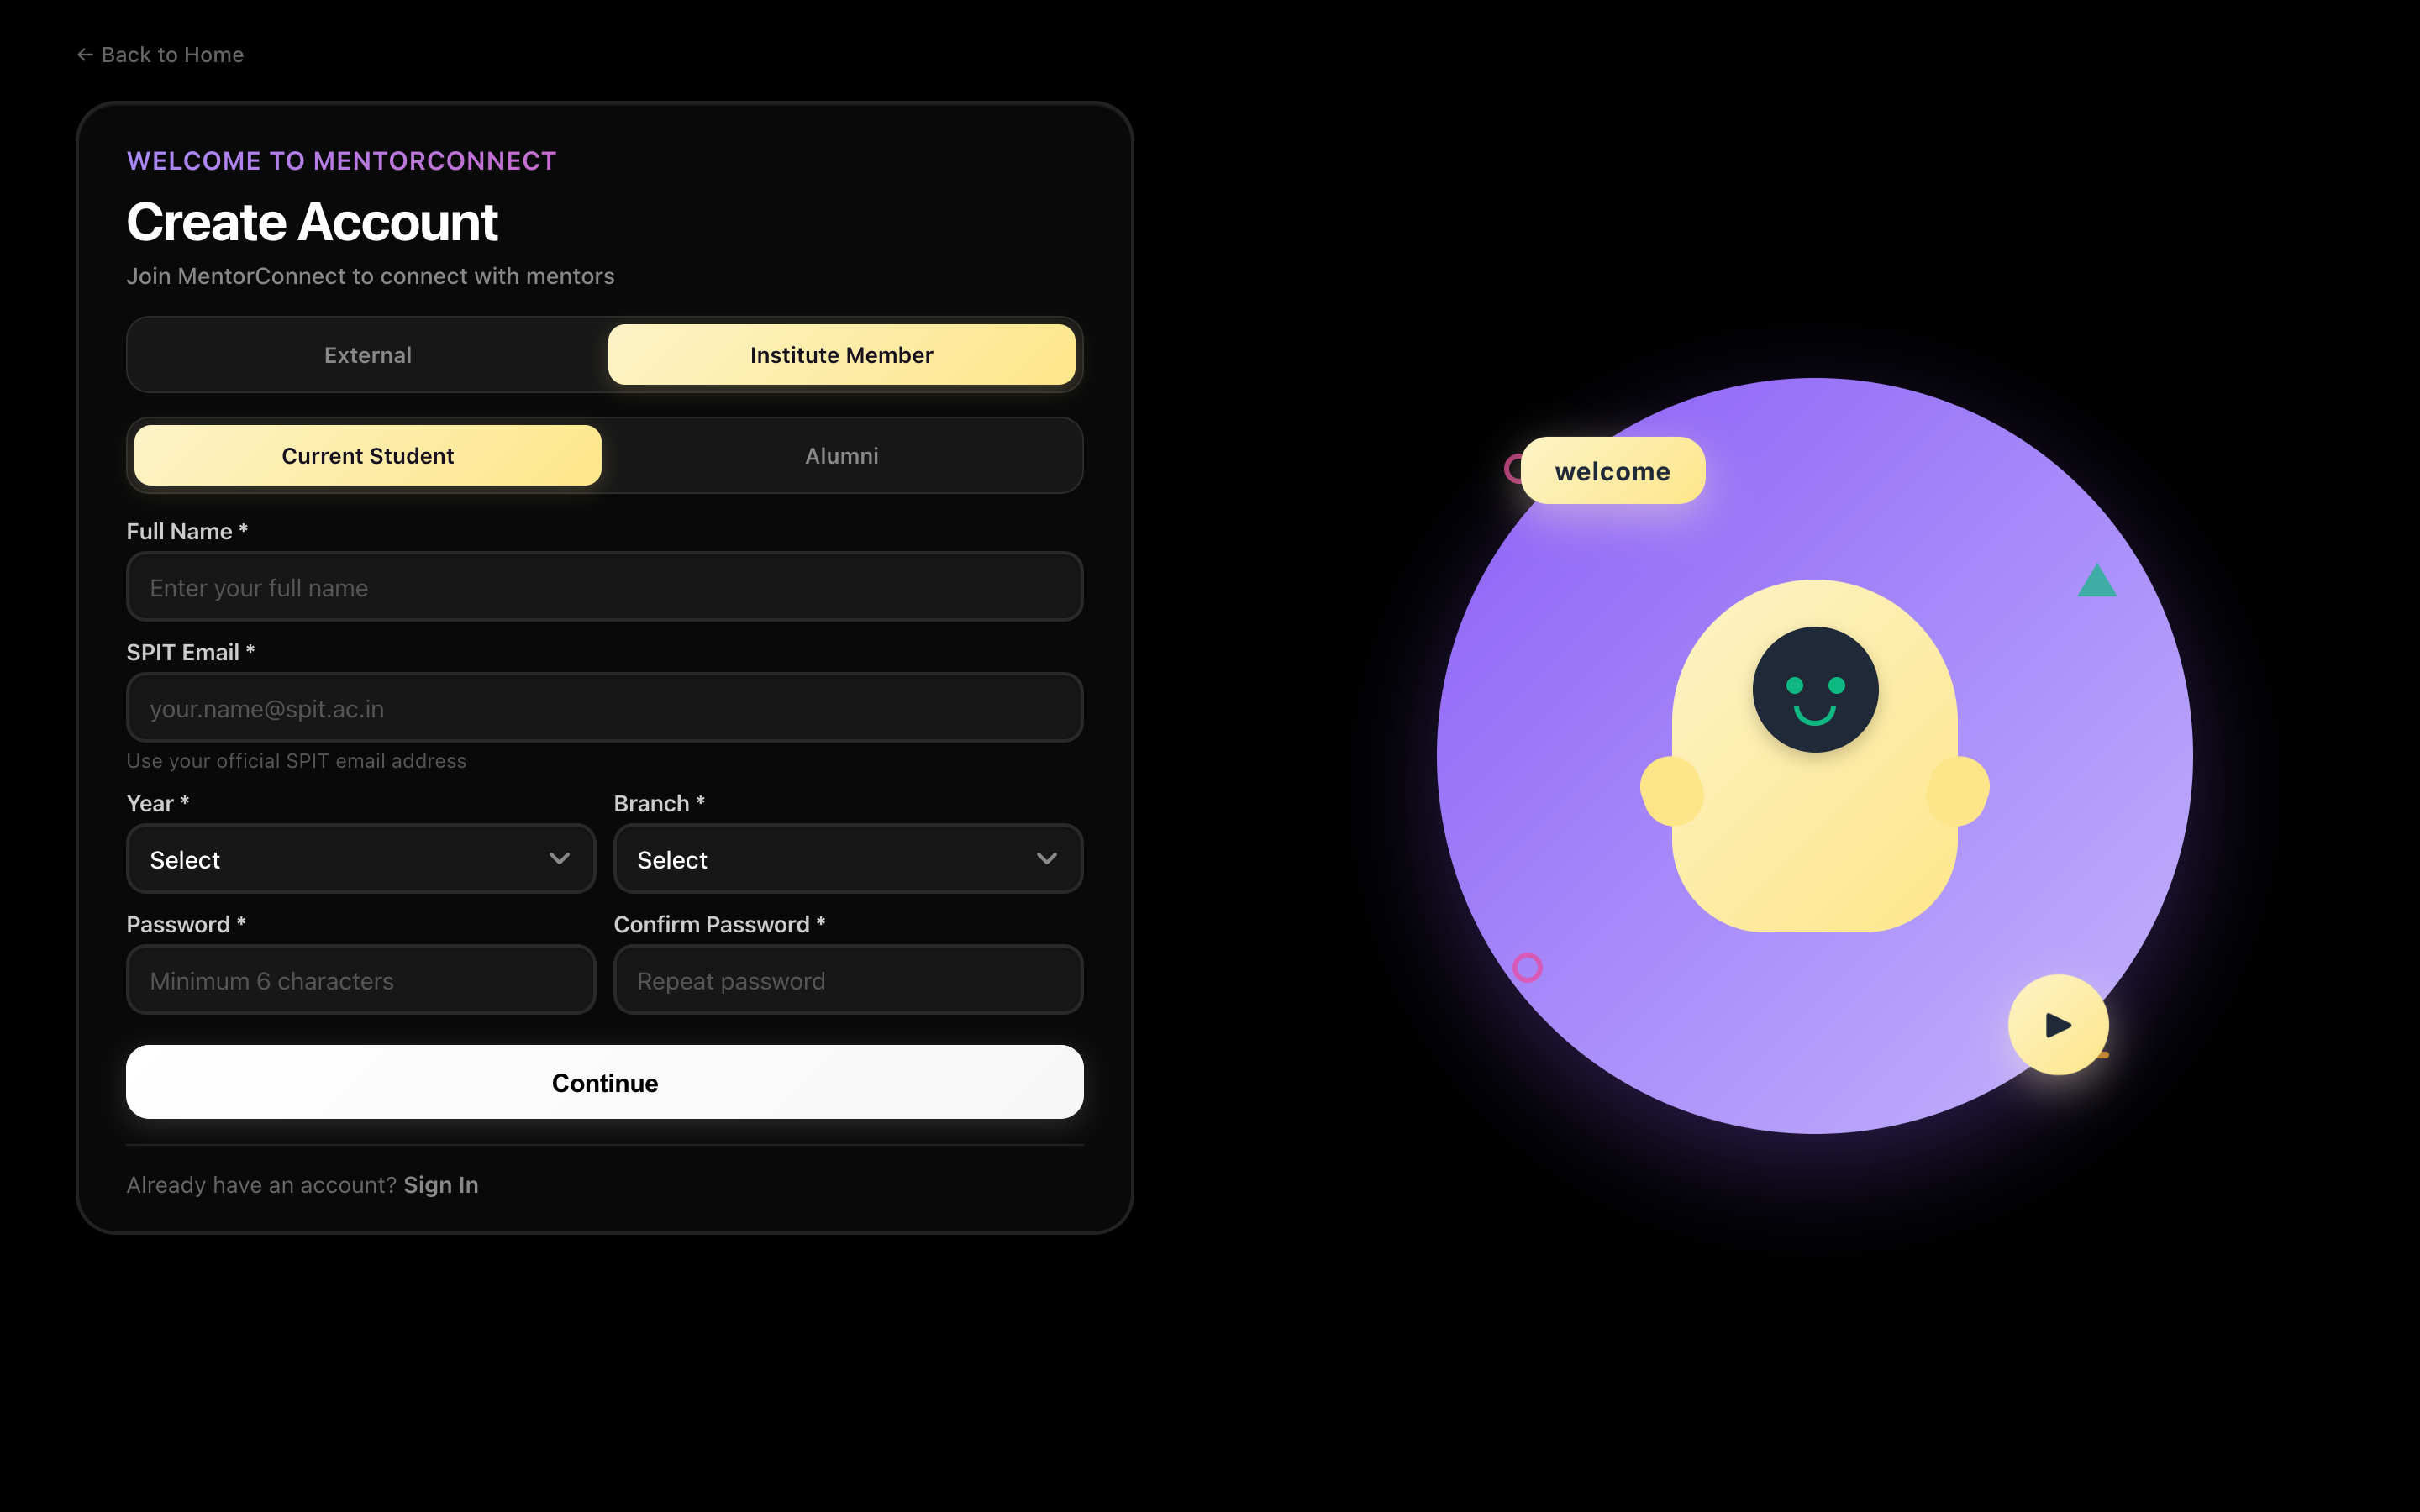
\includegraphics[width=\textwidth,height=0.82\textheight,keepaspectratio]{figures/register-institute-full.png}
\caption{Registration for institute members: current students or alumni, with institute email, year and branch}
\label{fig:ui-register-institute}
\end{figure}

\begin{figure}[htbp]
\centering
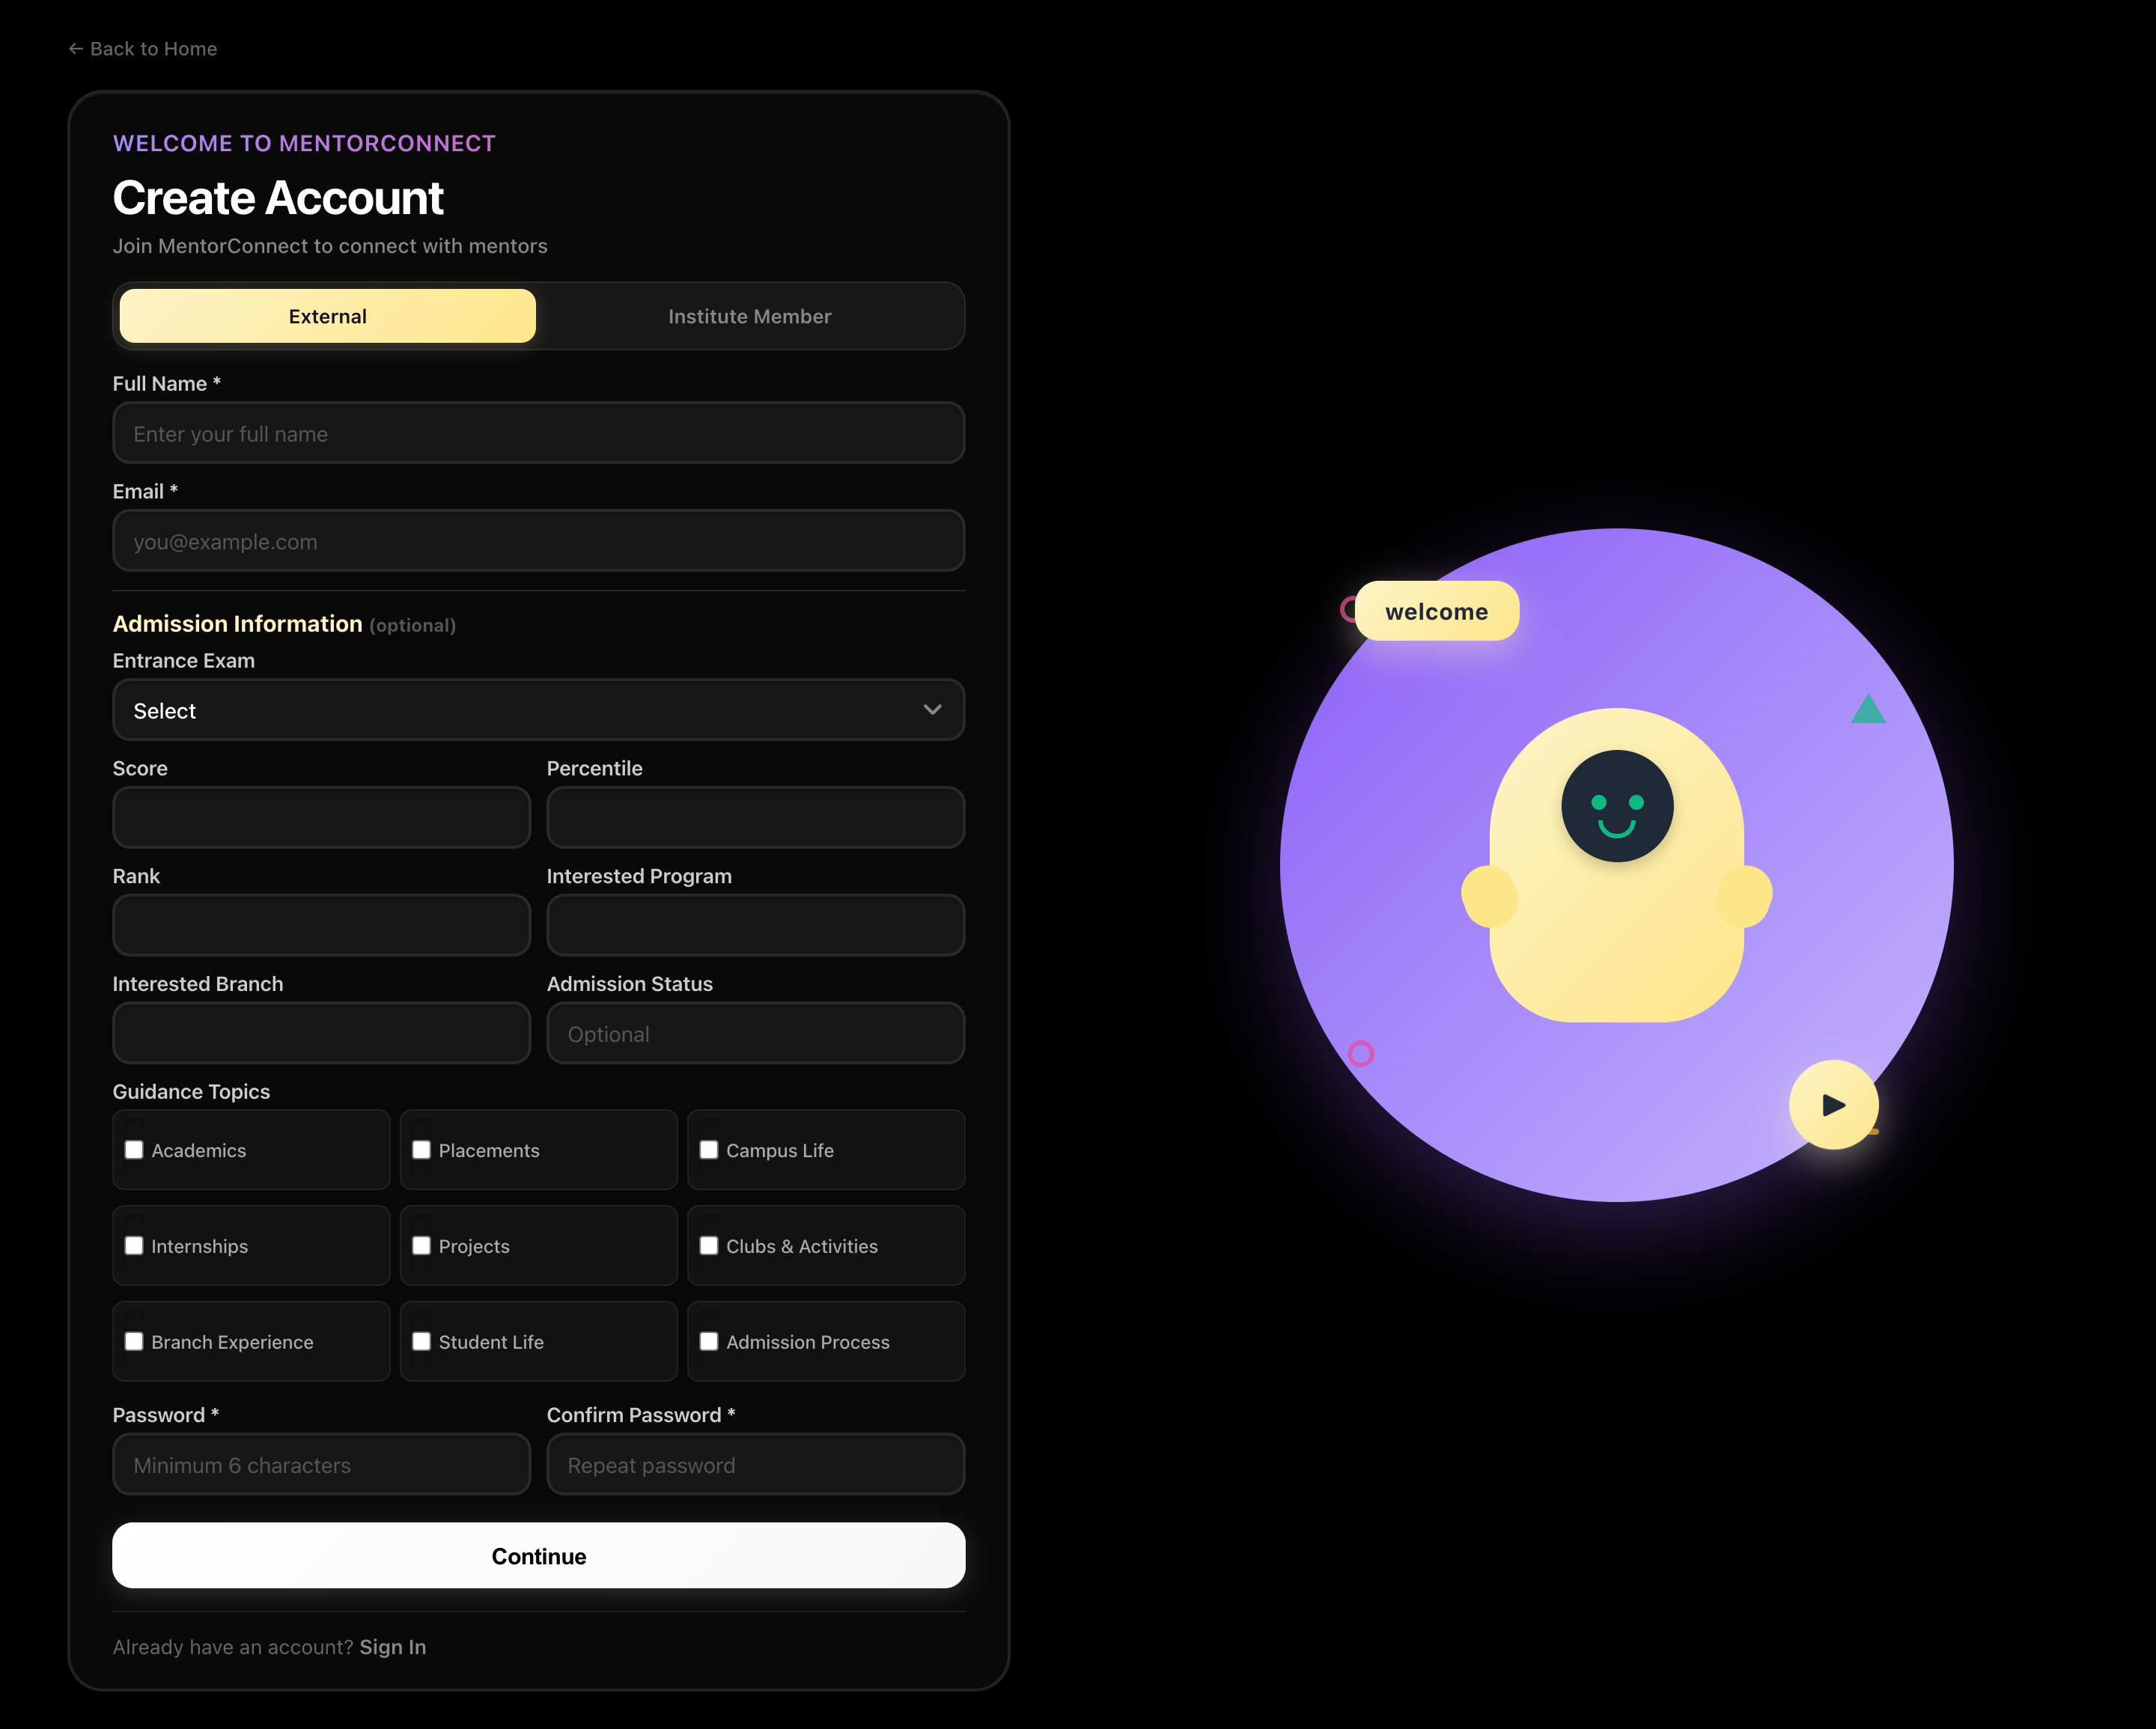
\includegraphics[width=\textwidth,height=0.82\textheight,keepaspectratio]{figures/register-full.png}
\caption{Registration for external learners, with optional admission information and guidance topics}
\label{fig:ui-register-external}
\end{figure}

Registration offers two paths. Institute members register as current students or alumni with their official institute email, year and branch (Figure~\ref{fig:ui-register-institute}). External learners, such as prospective students, register with any email and can optionally add admission information, such as entrance exam, score, rank and the programme and branch they are interested in, along with the topics they want guidance on: academics, placements, internships, projects, campus life and more (Figure~\ref{fig:ui-register-external}). Every new account is verified with a one-time password sent by email.

\begin{figure}[htbp]
\centering
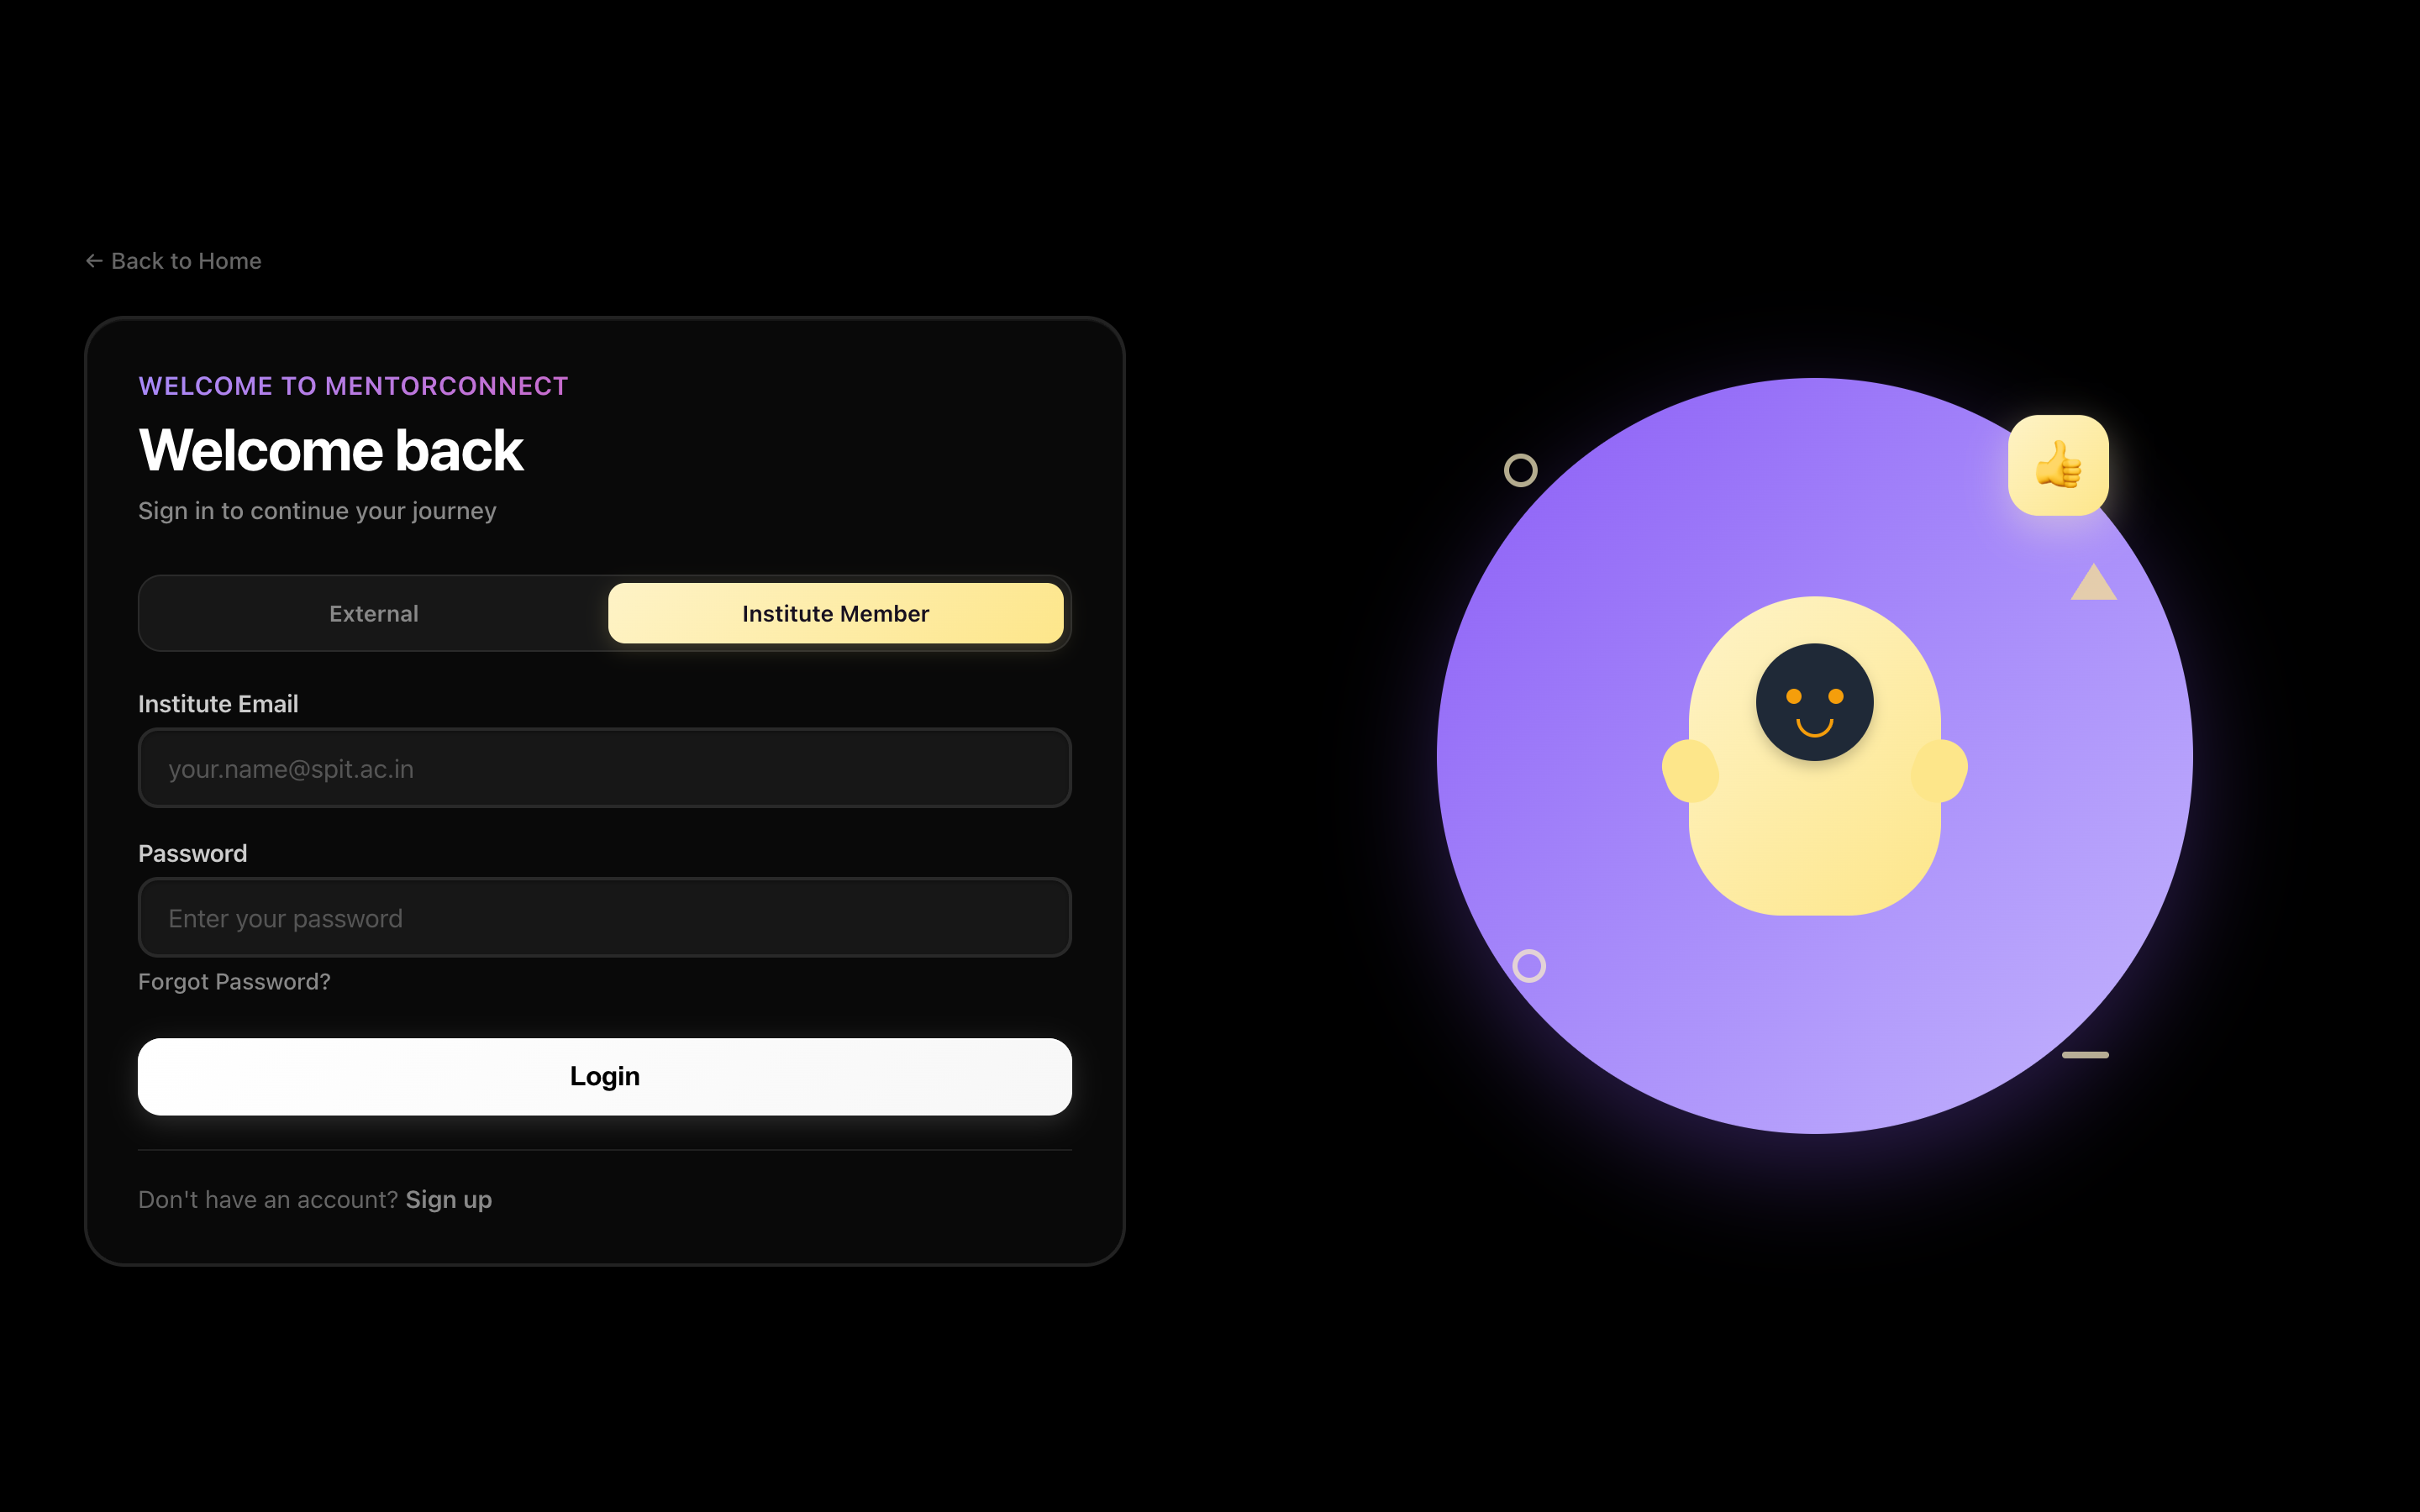
\includegraphics[width=0.95\textwidth]{figures/login.png}
\caption{Login page for institute members}
\label{fig:ui-login}
\end{figure}

\begin{figure}[htbp]
\centering
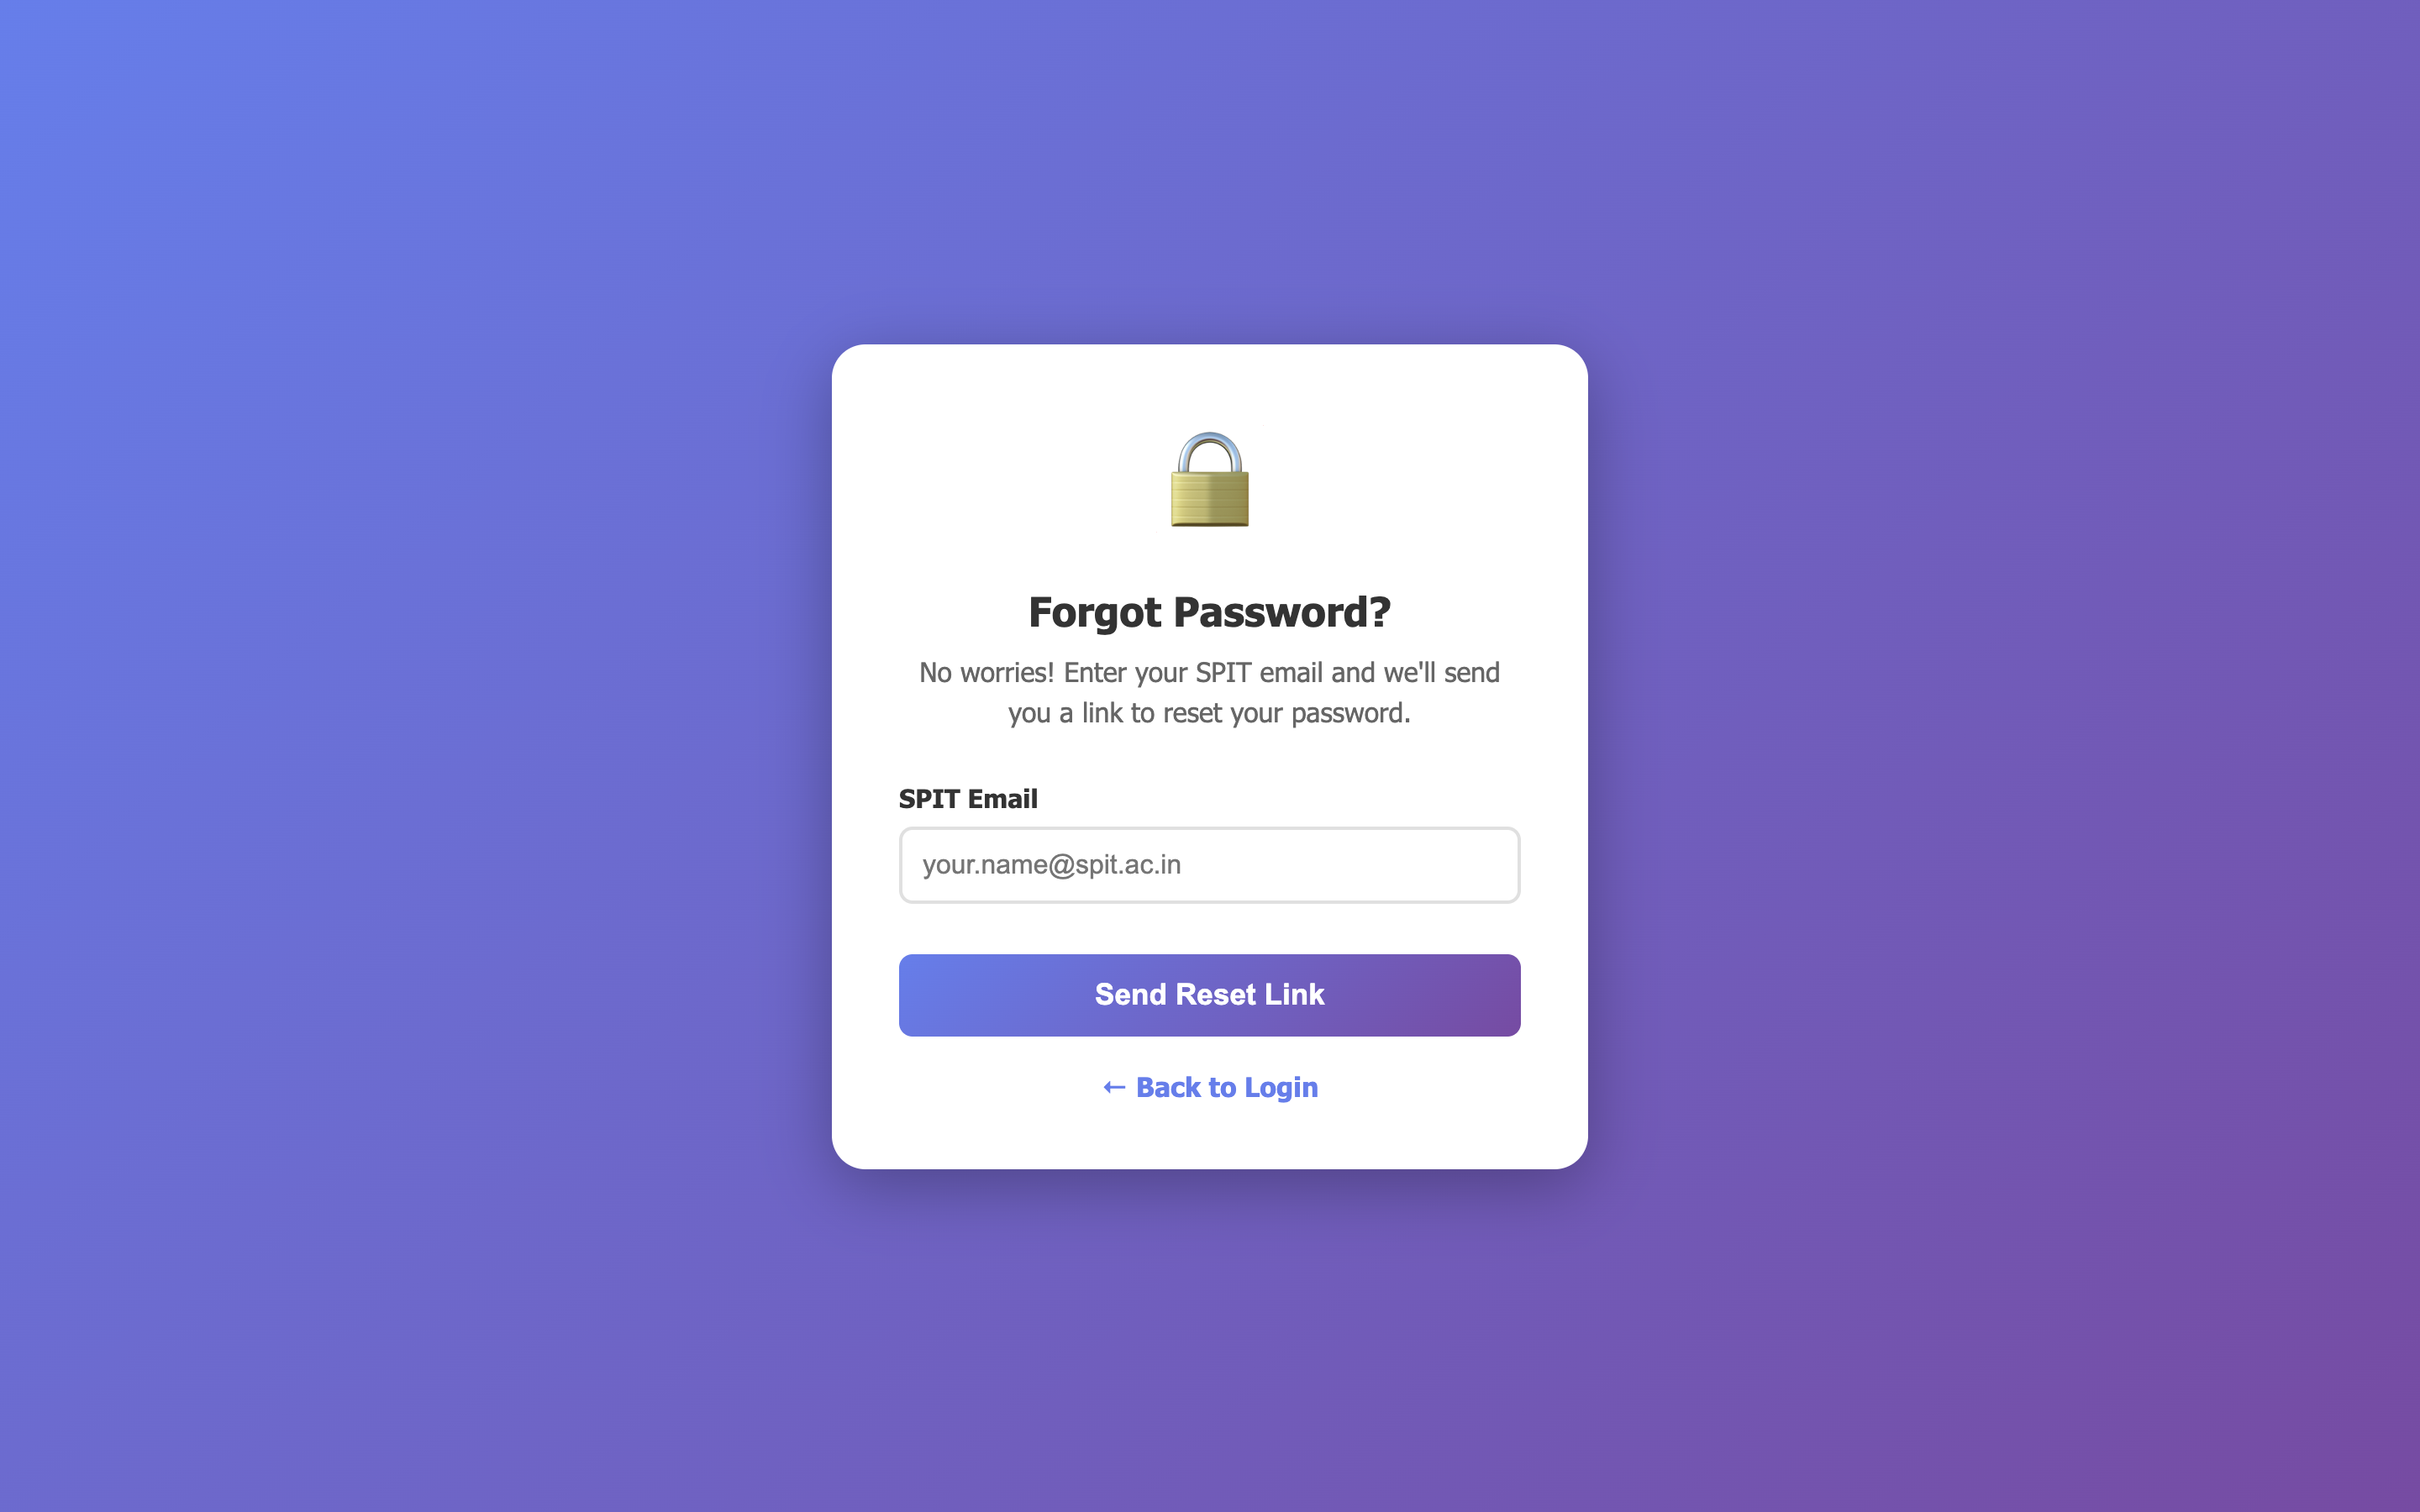
\includegraphics[width=0.95\textwidth]{figures/forgot-password.png}
\caption{Password recovery through the institute email}
\label{fig:ui-forgot}
\end{figure}

Students sign in after choosing their account type (Figure~\ref{fig:ui-login}). A student who forgets their password can request a reset link at their institute email (Figure~\ref{fig:ui-forgot}).

\subsection{Home, Feed and Notifications}
\begin{figure}[htbp]
\centering
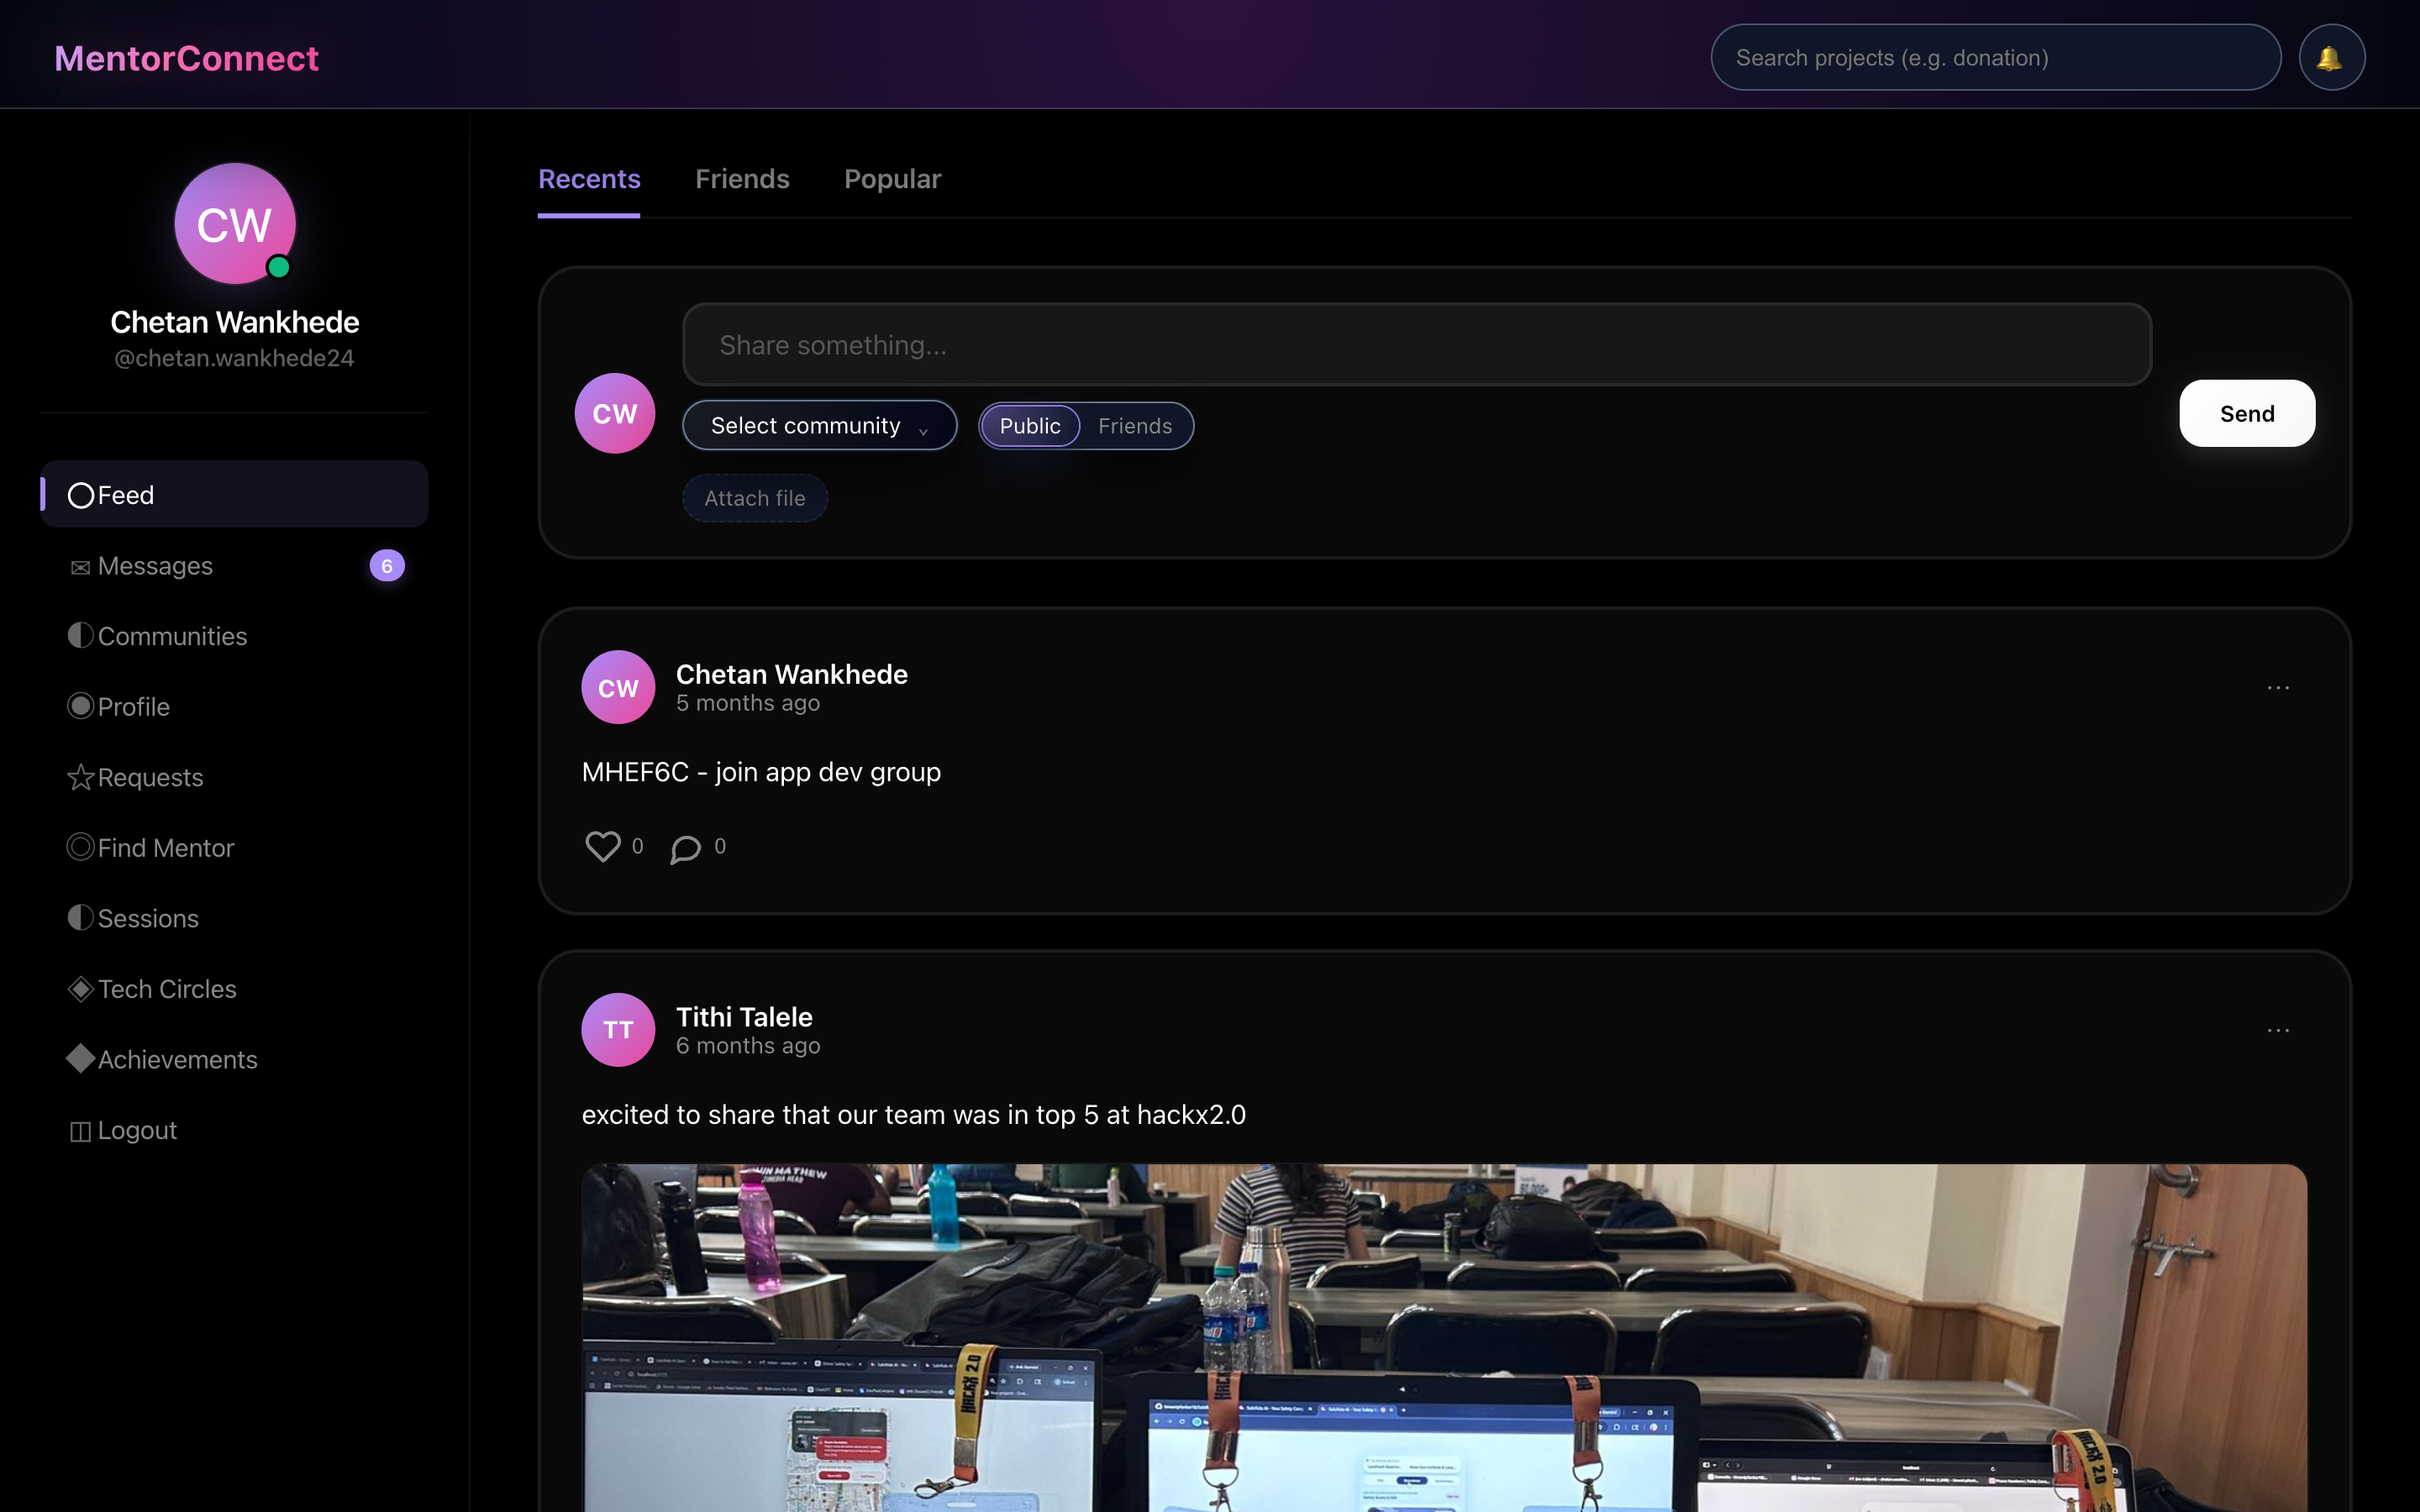
\includegraphics[width=0.95\textwidth]{figures/feed.png}
\caption{Home feed with posts and the main navigation}
\label{fig:ui-feed}
\end{figure}

\begin{figure}[htbp]
\centering
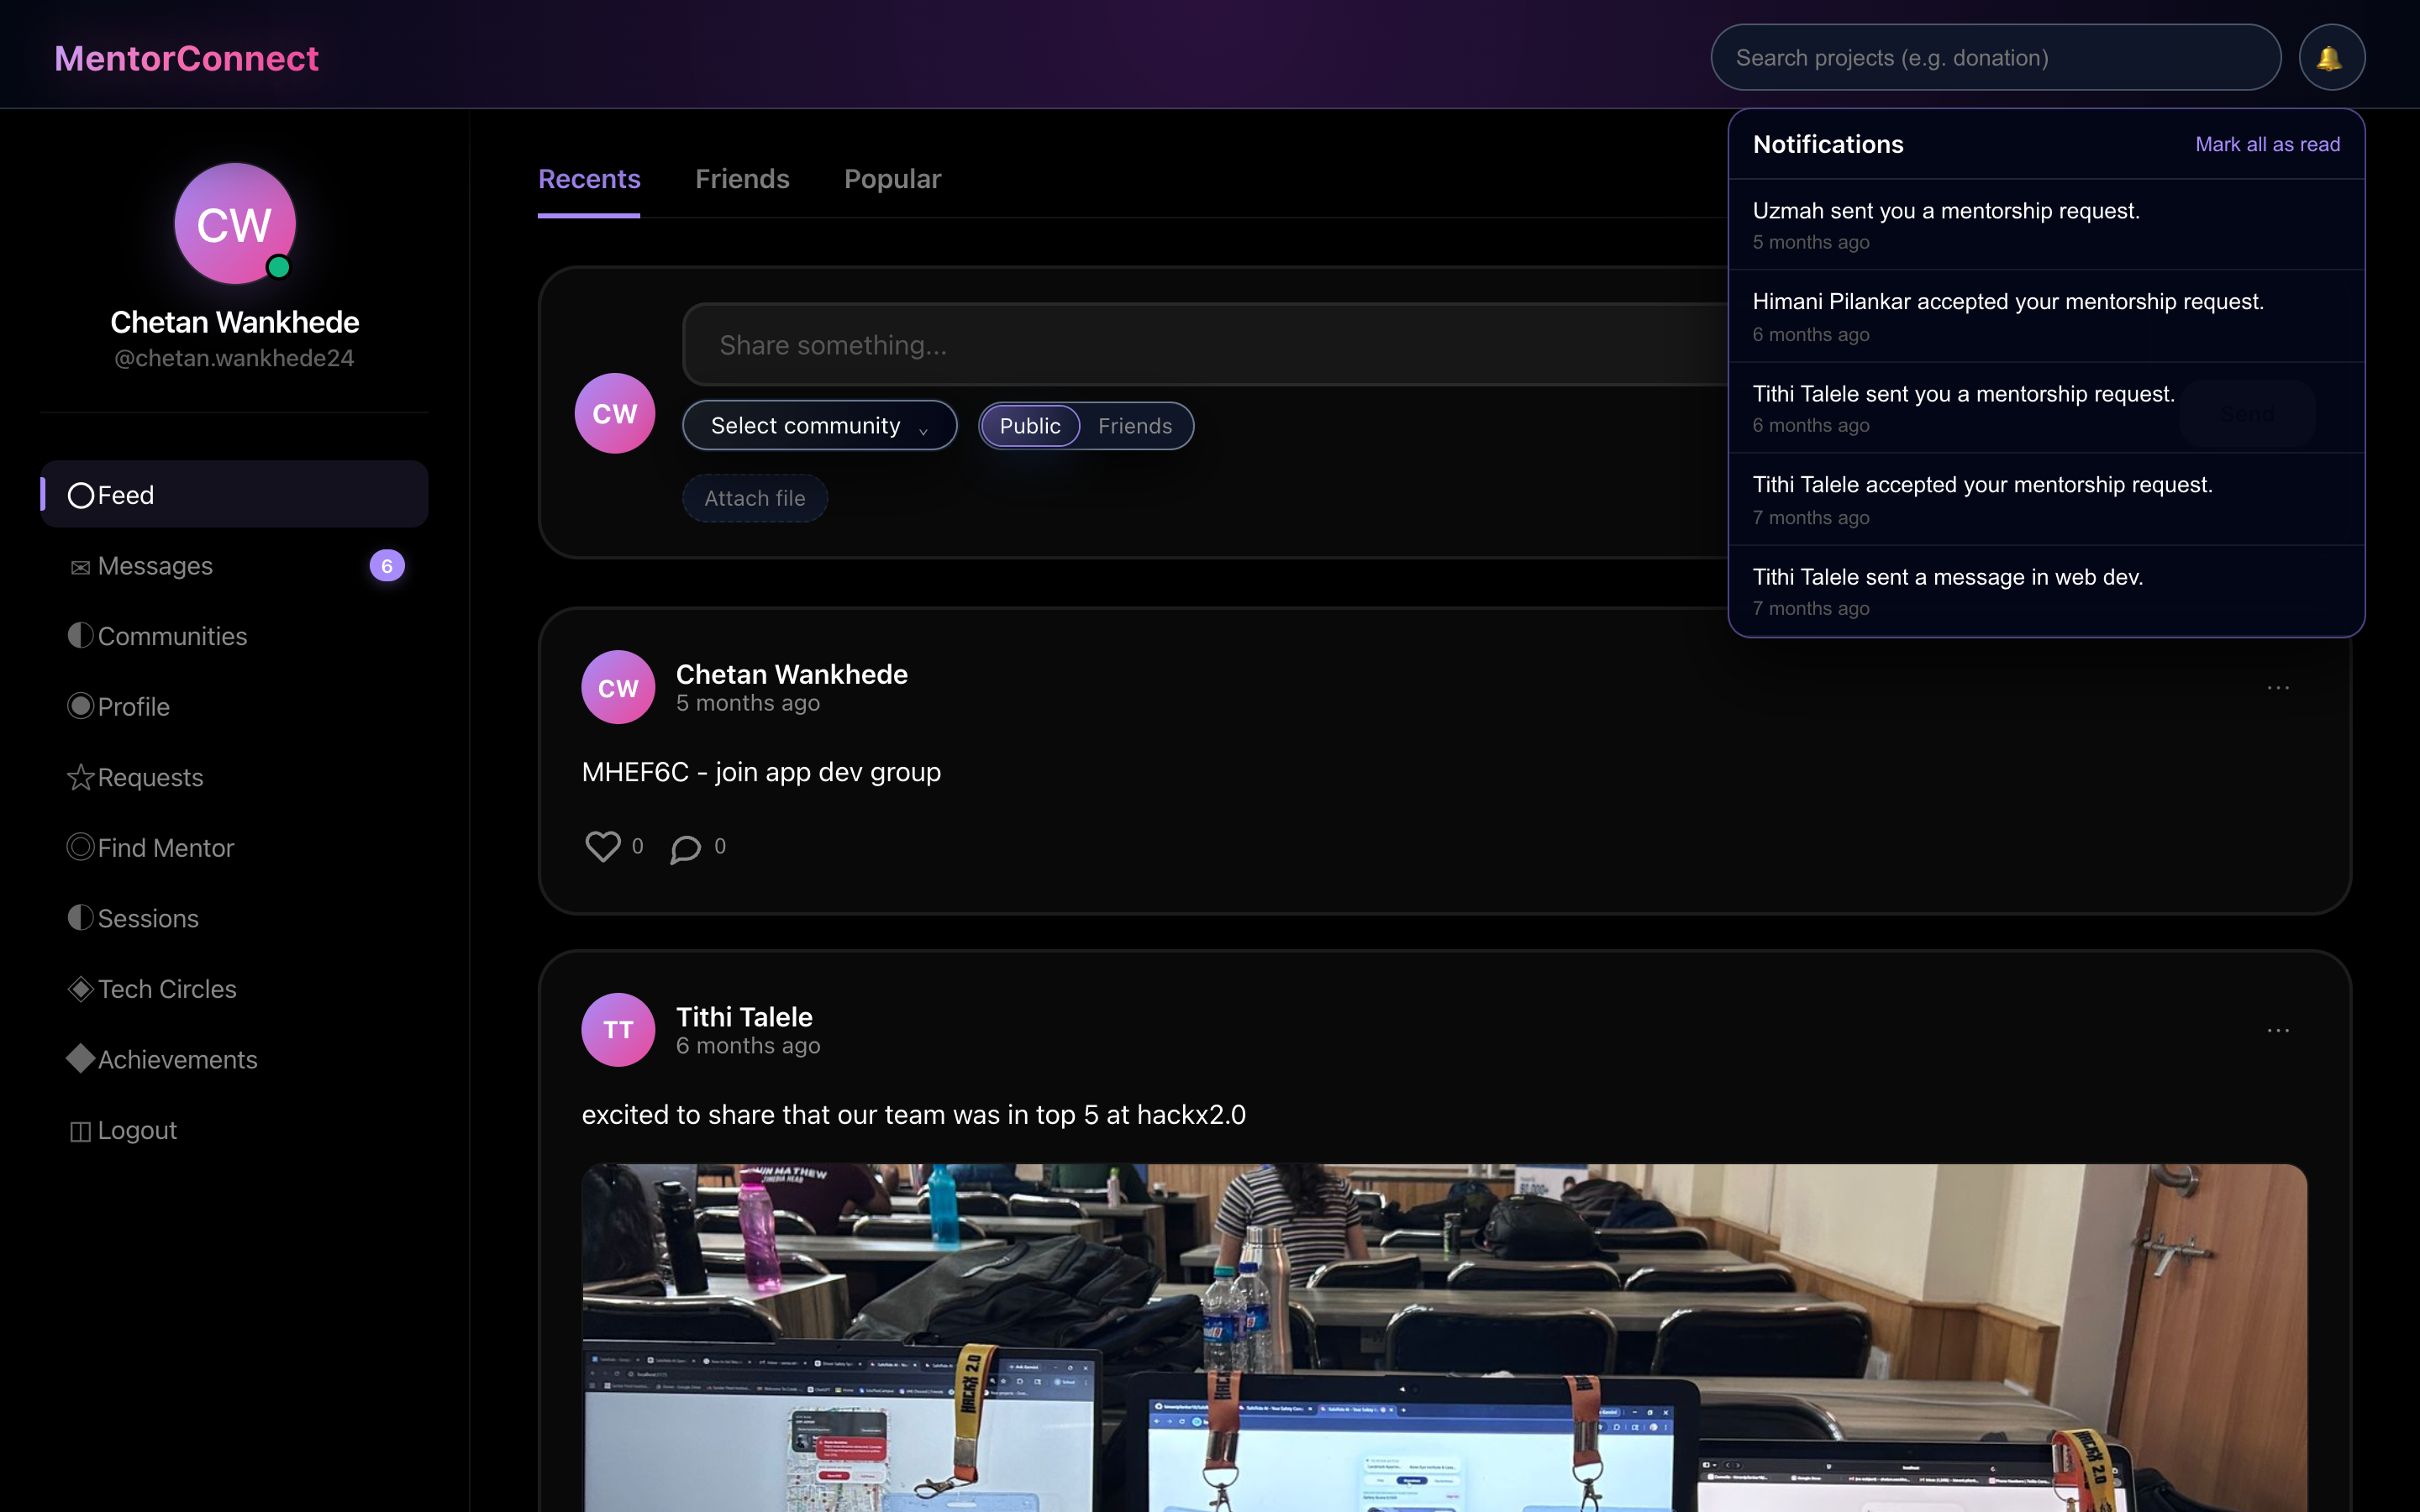
\includegraphics[width=0.95\textwidth]{figures/notifications.png}
\caption{Notifications for mentorship requests, acceptances and messages}
\label{fig:ui-notifications}
\end{figure}

After signing in, the student lands on the home feed (Figure~\ref{fig:ui-feed}). Posts can be shared publicly or with friends, linked to a community, and can carry attachments; the Recents, Friends and Popular tabs change the order of the feed. The left navigation gives access to every module of the platform. The notification bell (Figure~\ref{fig:ui-notifications}) shows real-time alerts for mentorship requests, accepted requests and new messages.

\subsection{Profiles}
\begin{figure}[htbp]
\centering
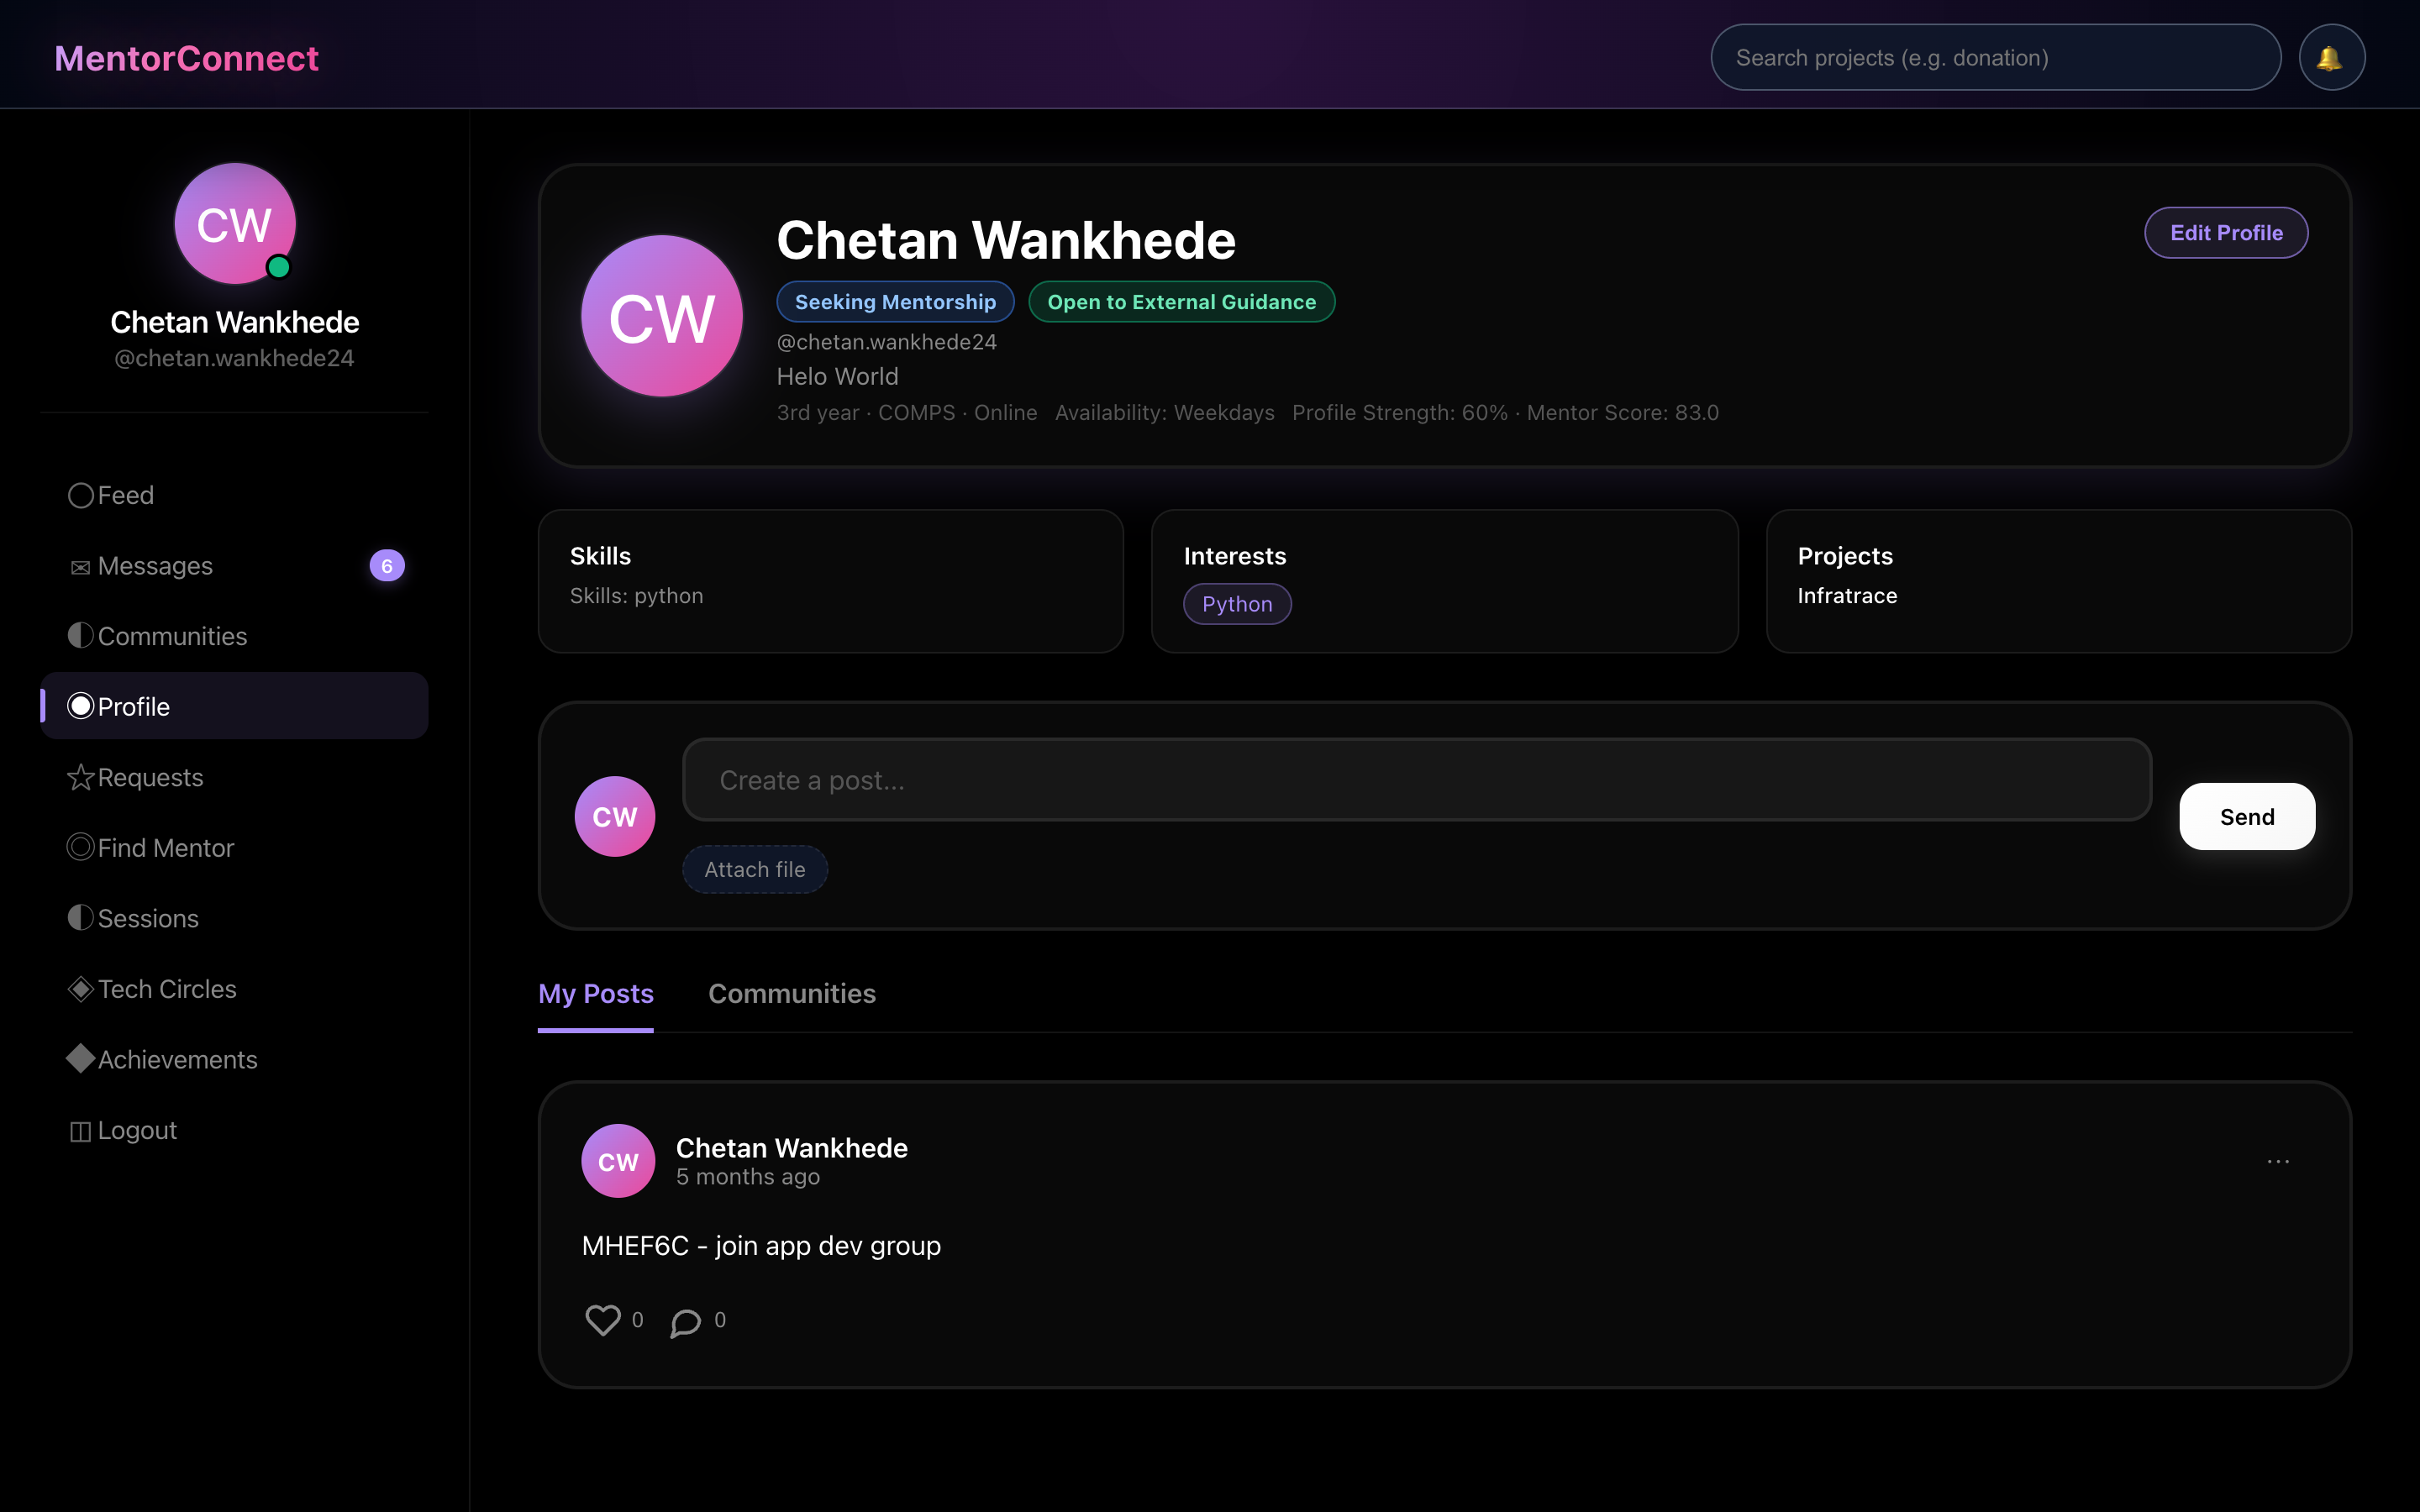
\includegraphics[width=0.95\textwidth]{figures/profile.png}
\caption{Student profile showing mentorship intent, availability, skills, interests and projects}
\label{fig:ui-profile}
\end{figure}

\begin{figure}[htbp]
\centering
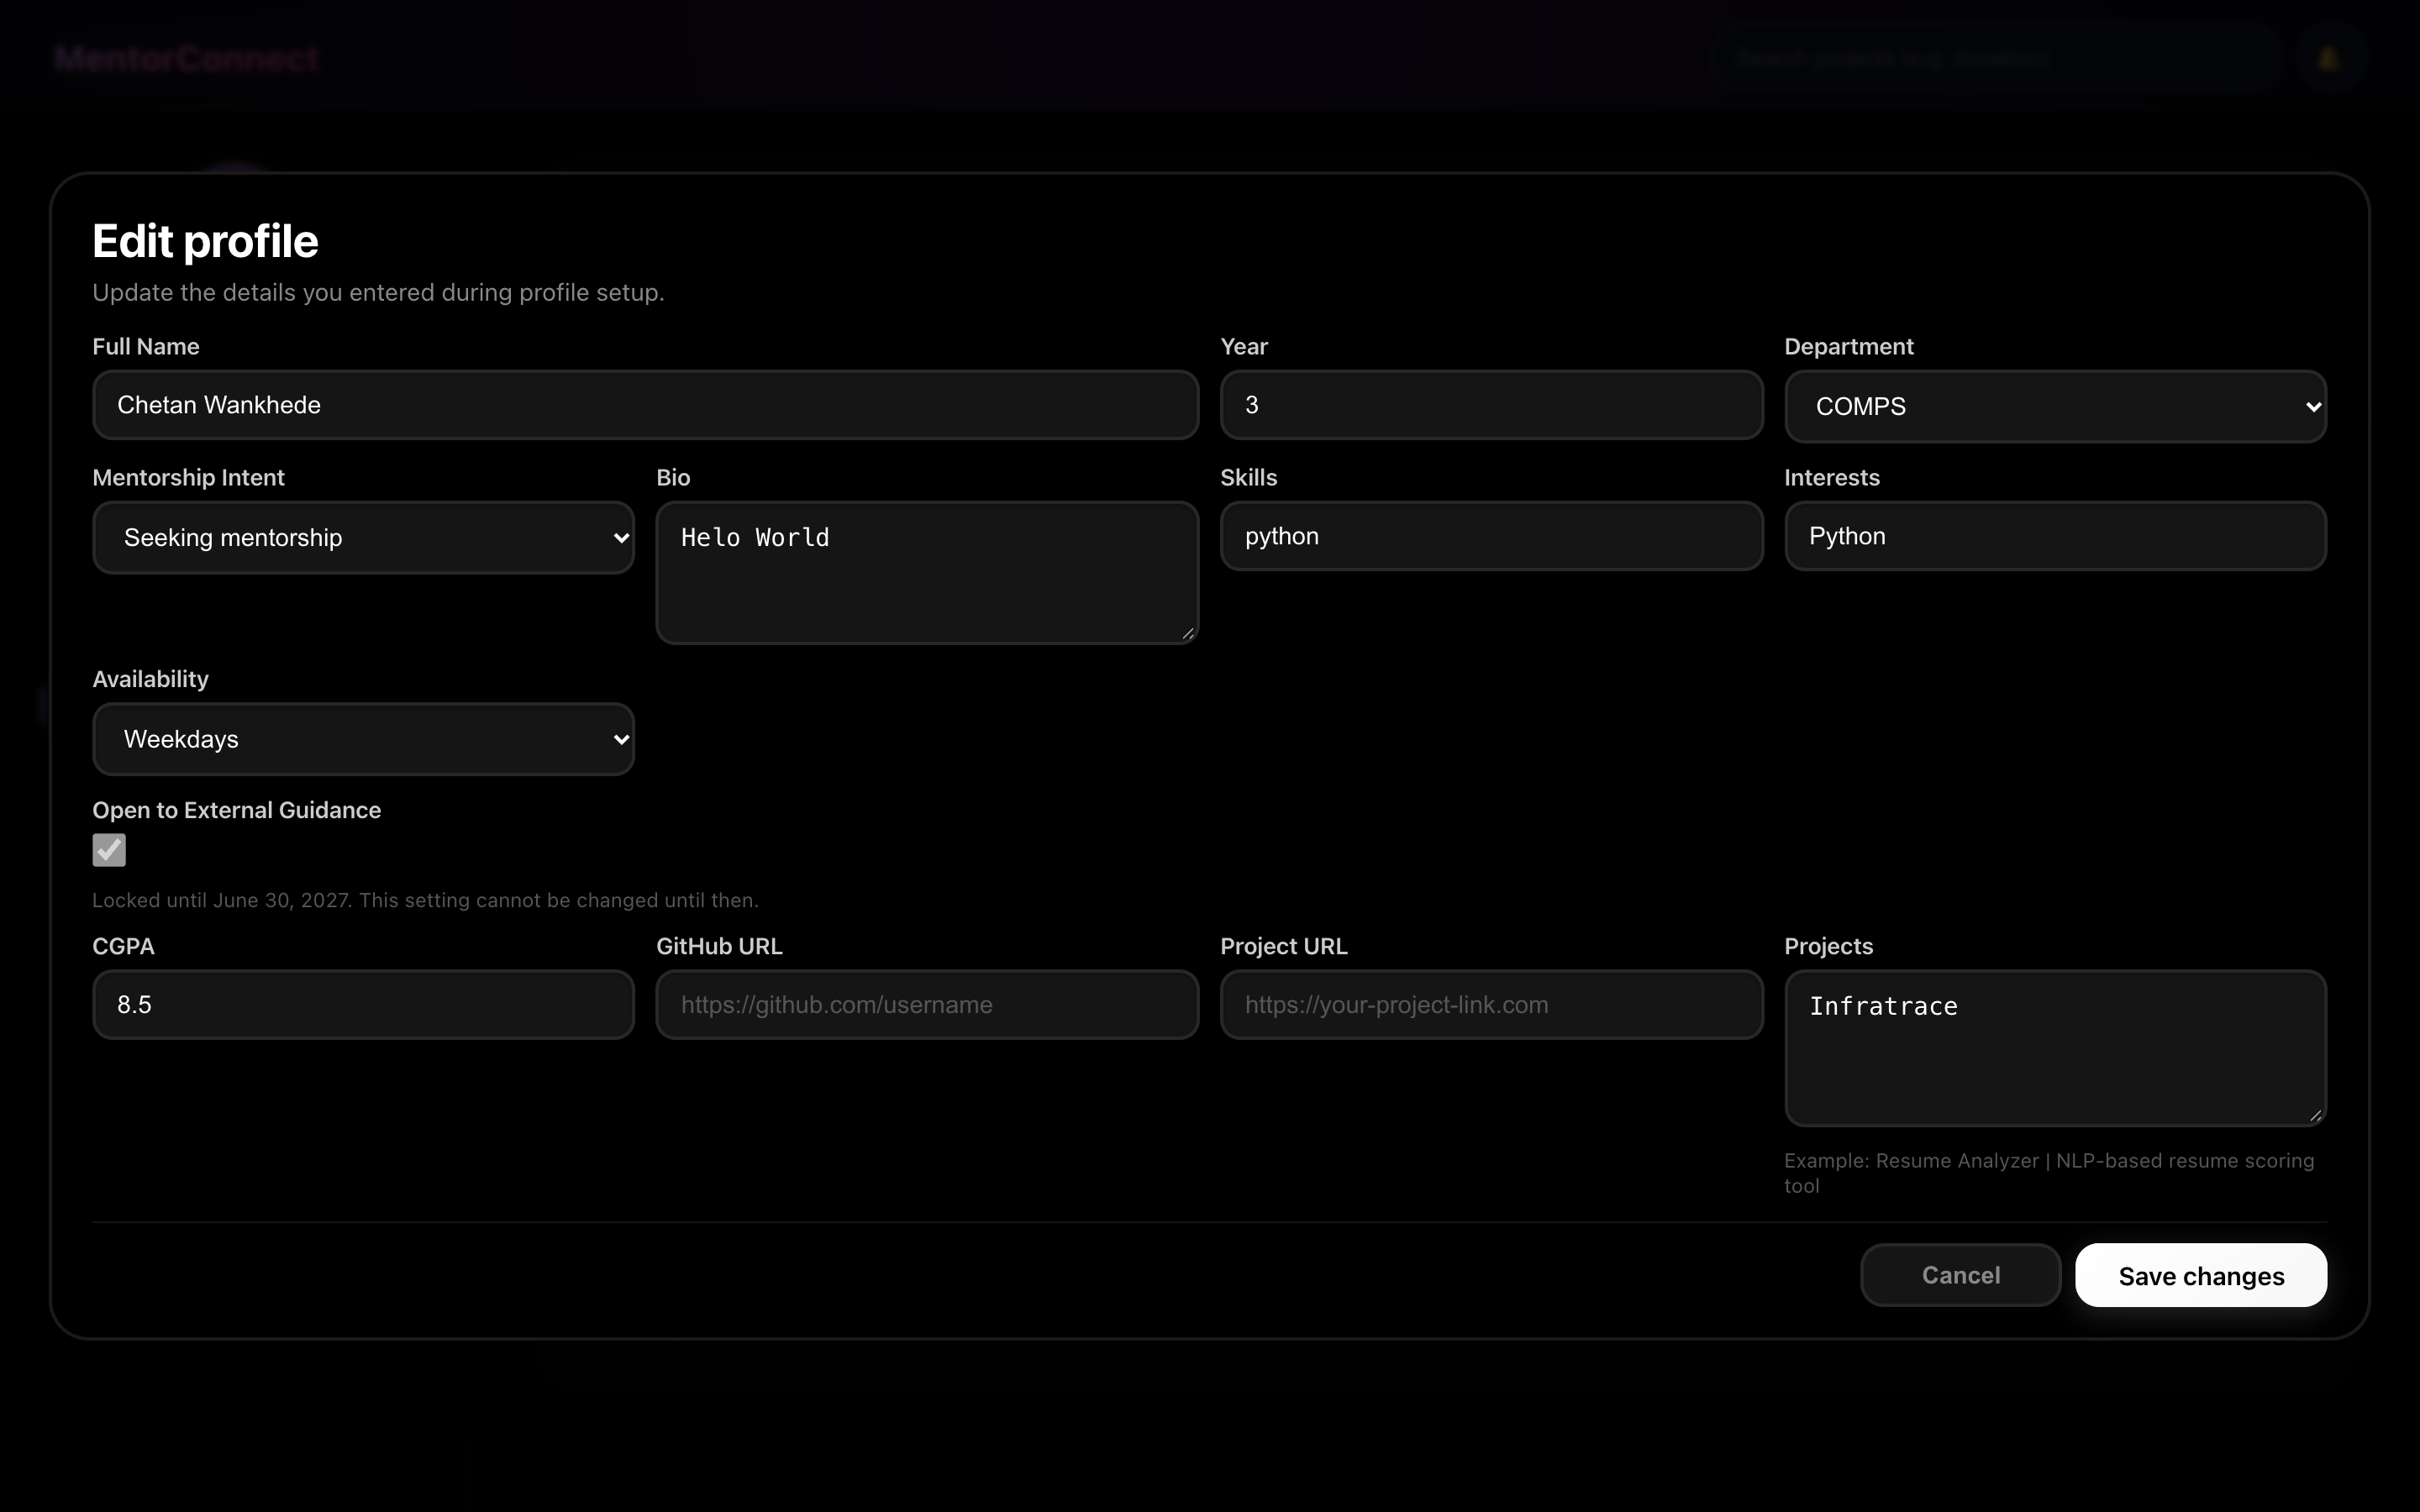
\includegraphics[width=0.95\textwidth]{figures/edit-profile.png}
\caption{Editing a profile, including mentorship intent and the External Guidance consent}
\label{fig:ui-edit-profile}
\end{figure}

\begin{figure}[htbp]
\centering
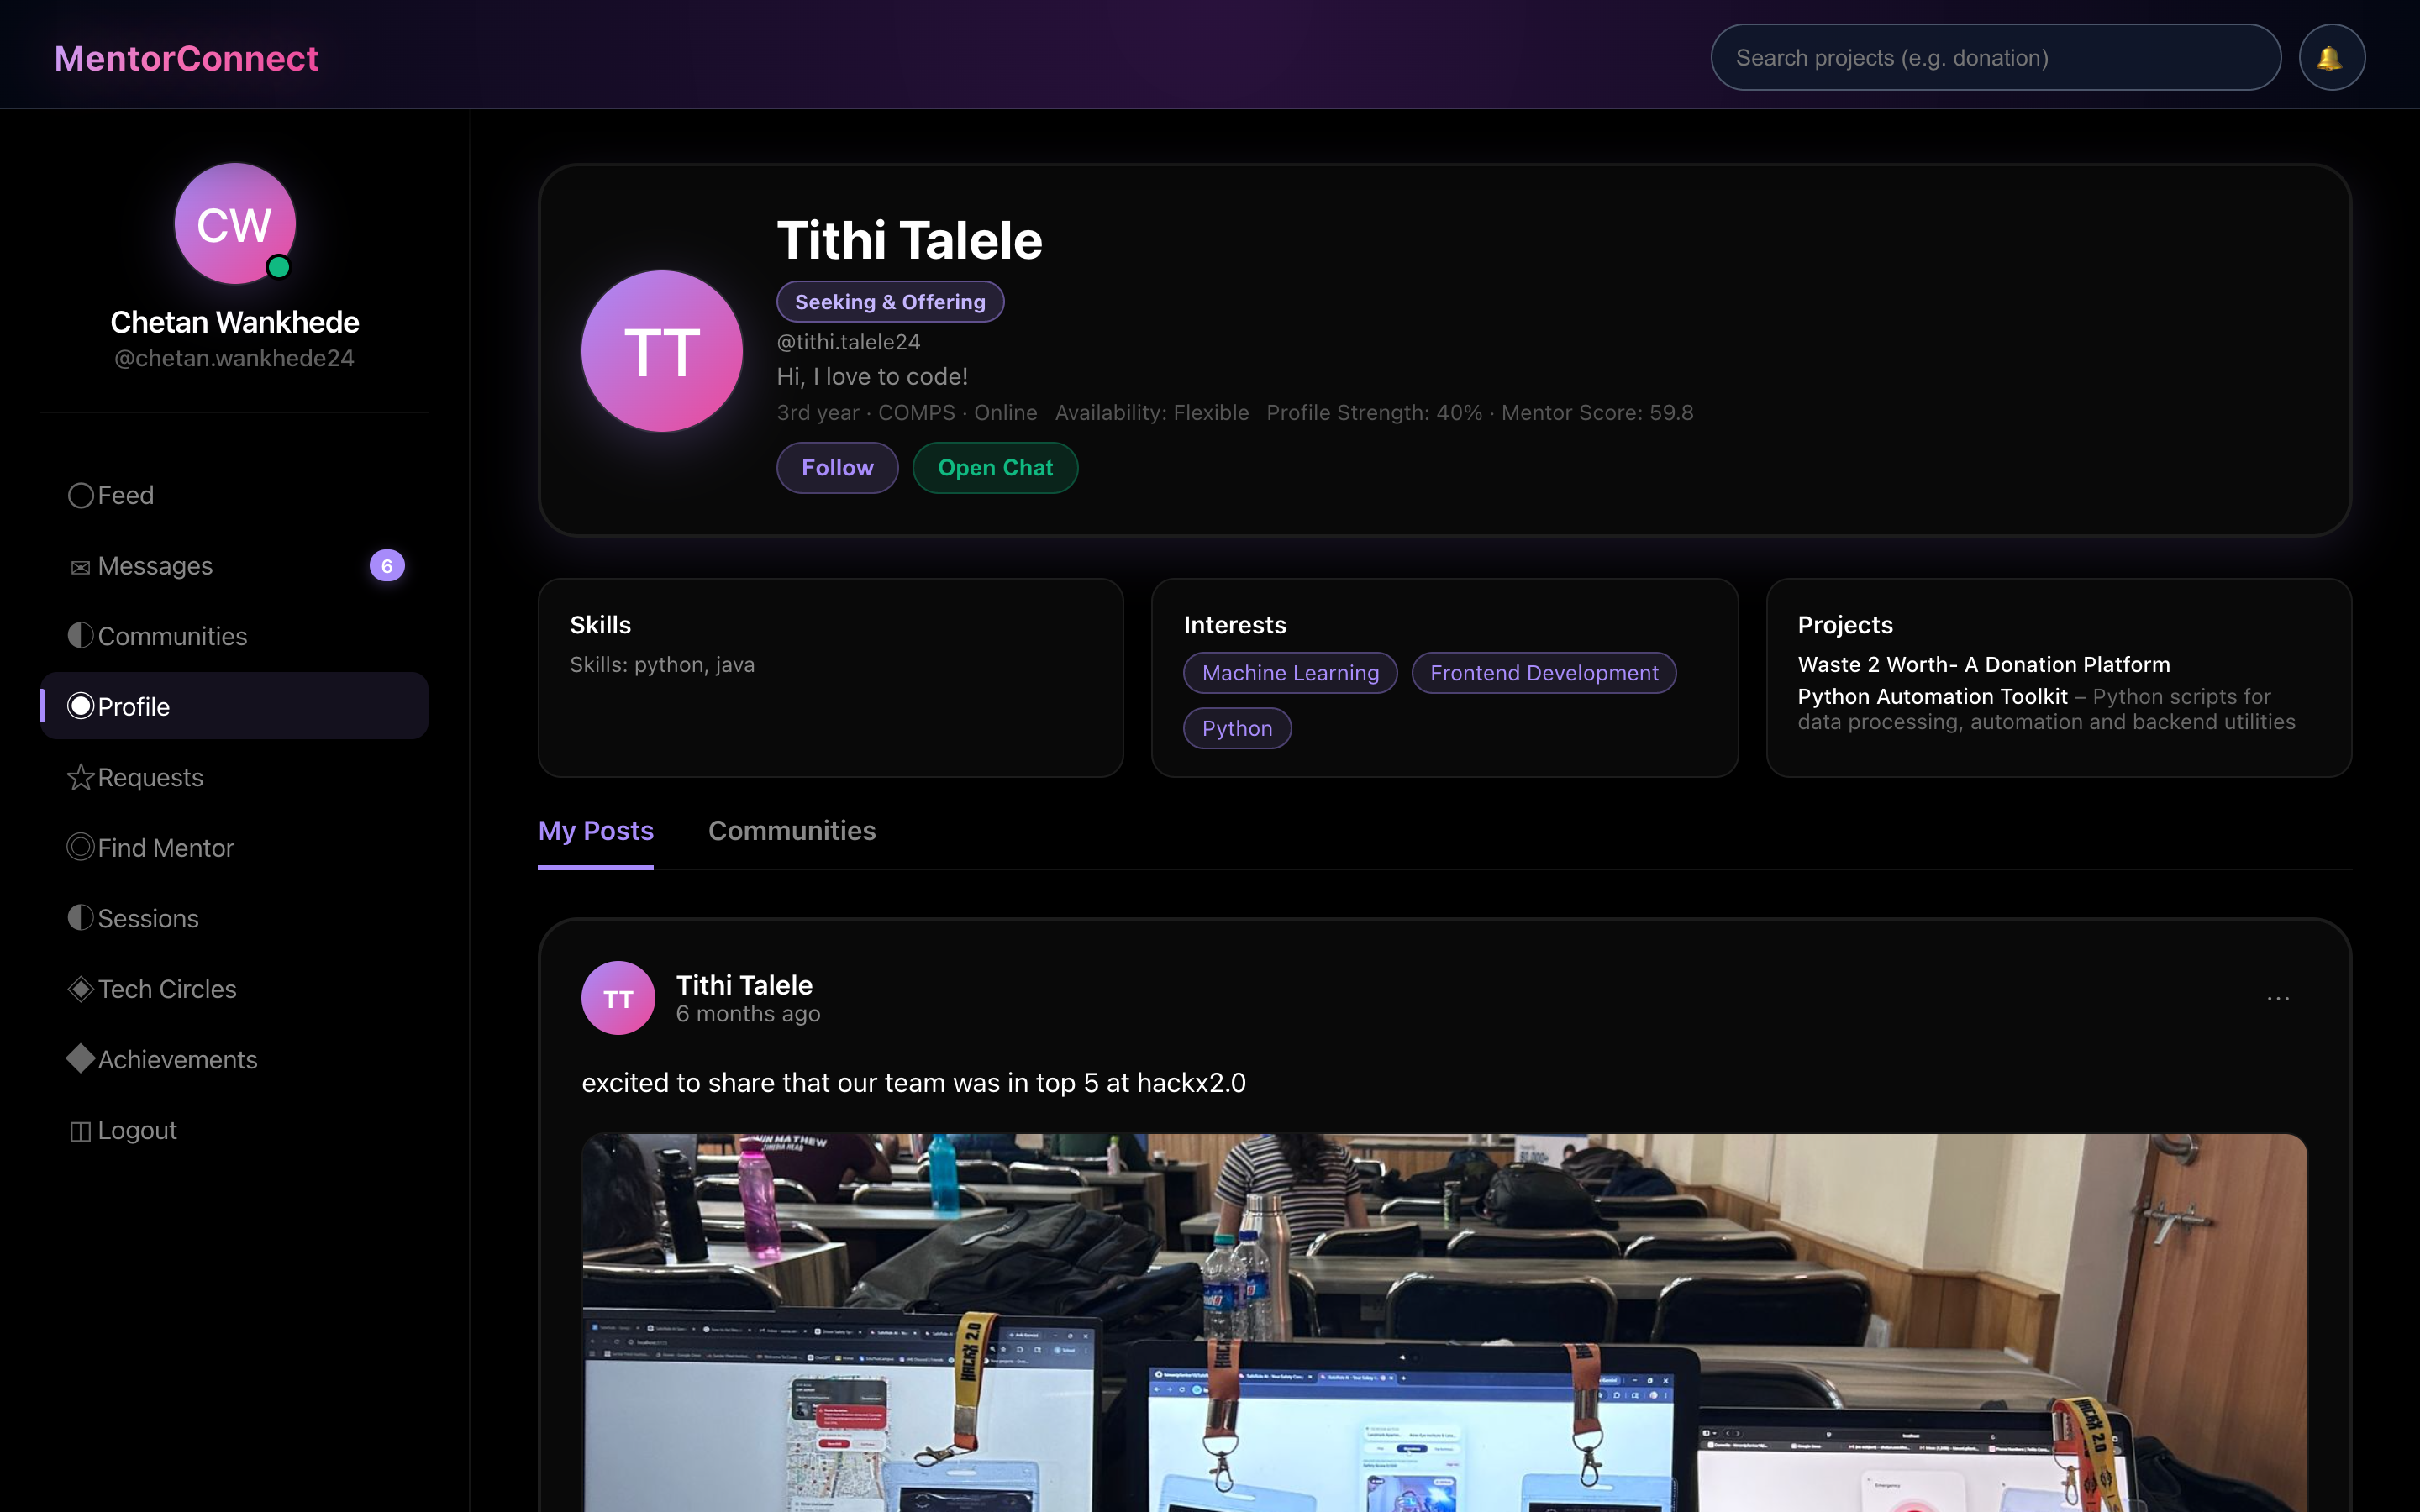
\includegraphics[width=0.95\textwidth]{figures/user-profile.png}
\caption{Viewing another student's profile}
\label{fig:ui-user-profile}
\end{figure}

The profile page (Figure~\ref{fig:ui-profile}) shows the student's mentorship intent, External Guidance status, year, department, availability, profile strength, mentor score, skills, interests and projects; these fields are the inputs to the recommendation engine. The edit form (Figure~\ref{fig:ui-edit-profile}) updates them; once a mentor opts in to External Guidance, the choice is locked until the end of the academic year, as the form explains. Other students' profiles (Figure~\ref{fig:ui-user-profile}) show the same information with actions to follow the student, request mentorship or open an existing mentorship chat.

\subsection{Mentor Discovery and Mentorship}
\begin{figure}[htbp]
\centering
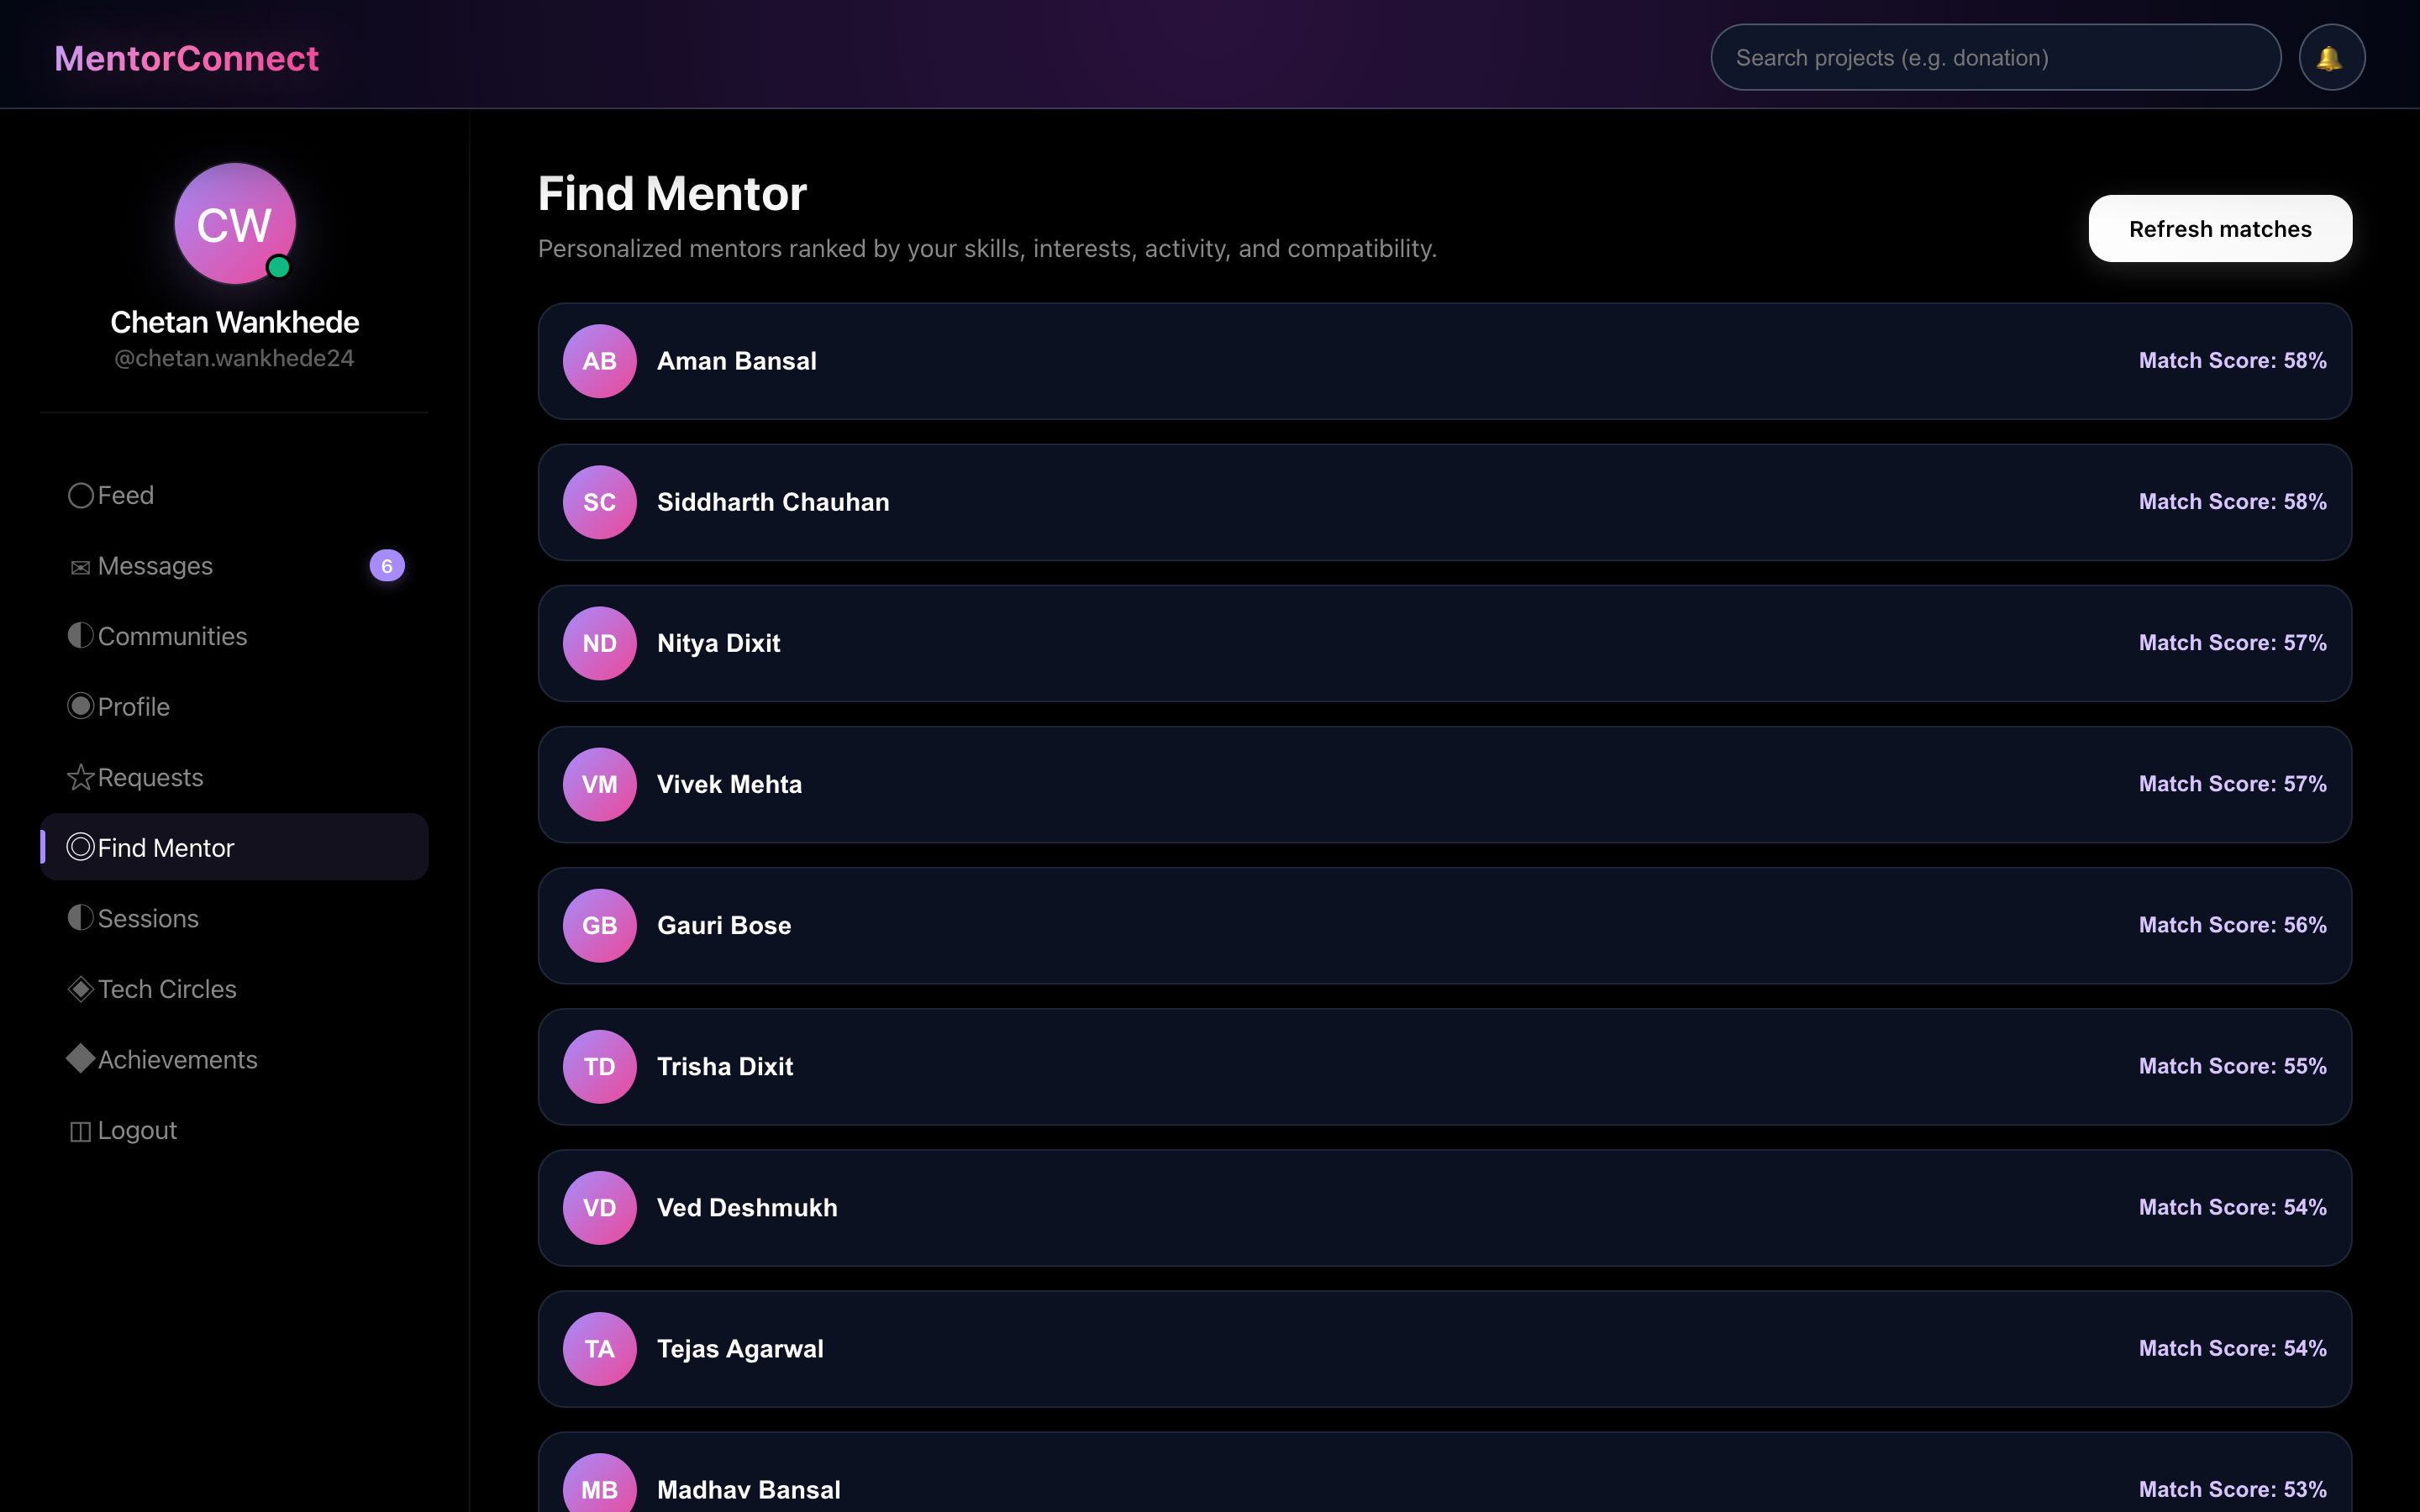
\includegraphics[width=0.95\textwidth]{figures/find-mentor.png}
\caption{Find Mentor: mentors ranked by the recommendation engine}
\label{fig:ui-findmentor-list}
\end{figure}

\begin{figure}[htbp]
\centering
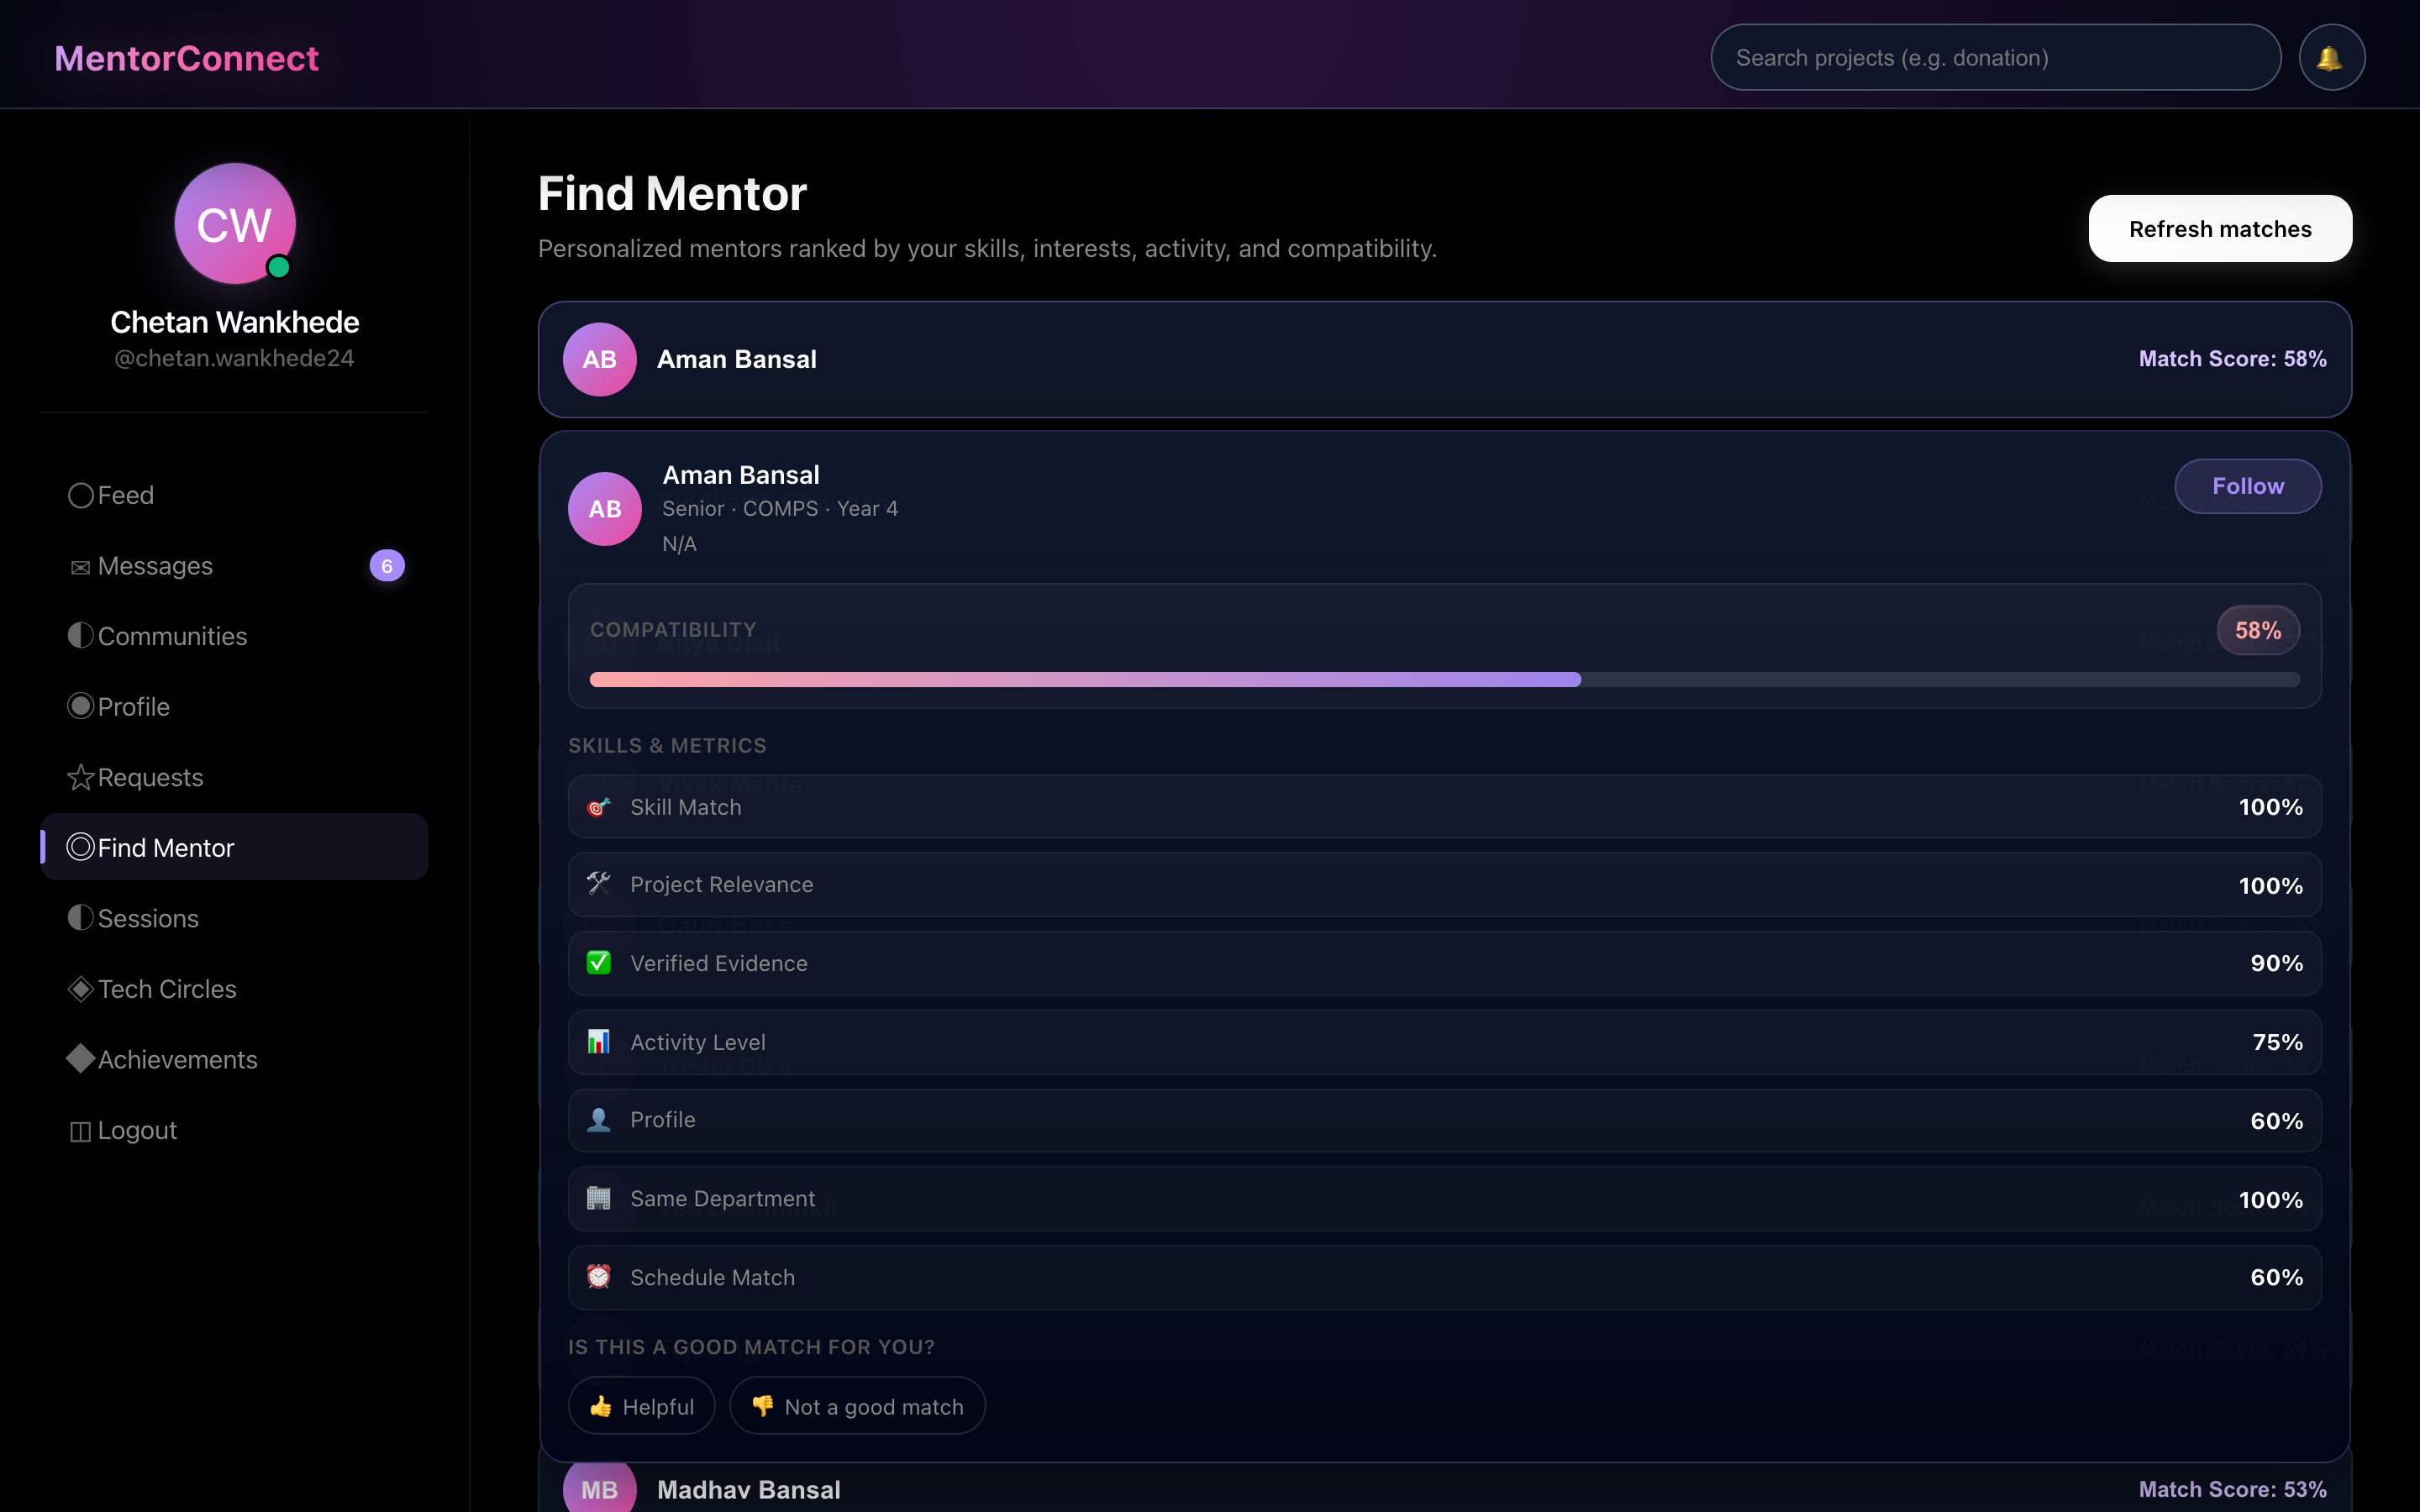
\includegraphics[width=0.95\textwidth]{figures/find-mentor-detail.png}
\caption{A recommendation opened to show its per-factor explanation and feedback buttons}
\label{fig:ui-findmentor}
\end{figure}

Find Mentor (Figure~\ref{fig:ui-findmentor-list}) lists mentors ranked by the recommendation engine with a match score for each. Opening a recommendation (Figure~\ref{fig:ui-findmentor}) reveals the explanation behind the score: skill match, project relevance, verified evidence, activity level, profile completeness, department and schedule match. The student can mark the recommendation as helpful or not a good match, and this feedback is logged together with the list for evaluation.

\begin{figure}[htbp]
\centering
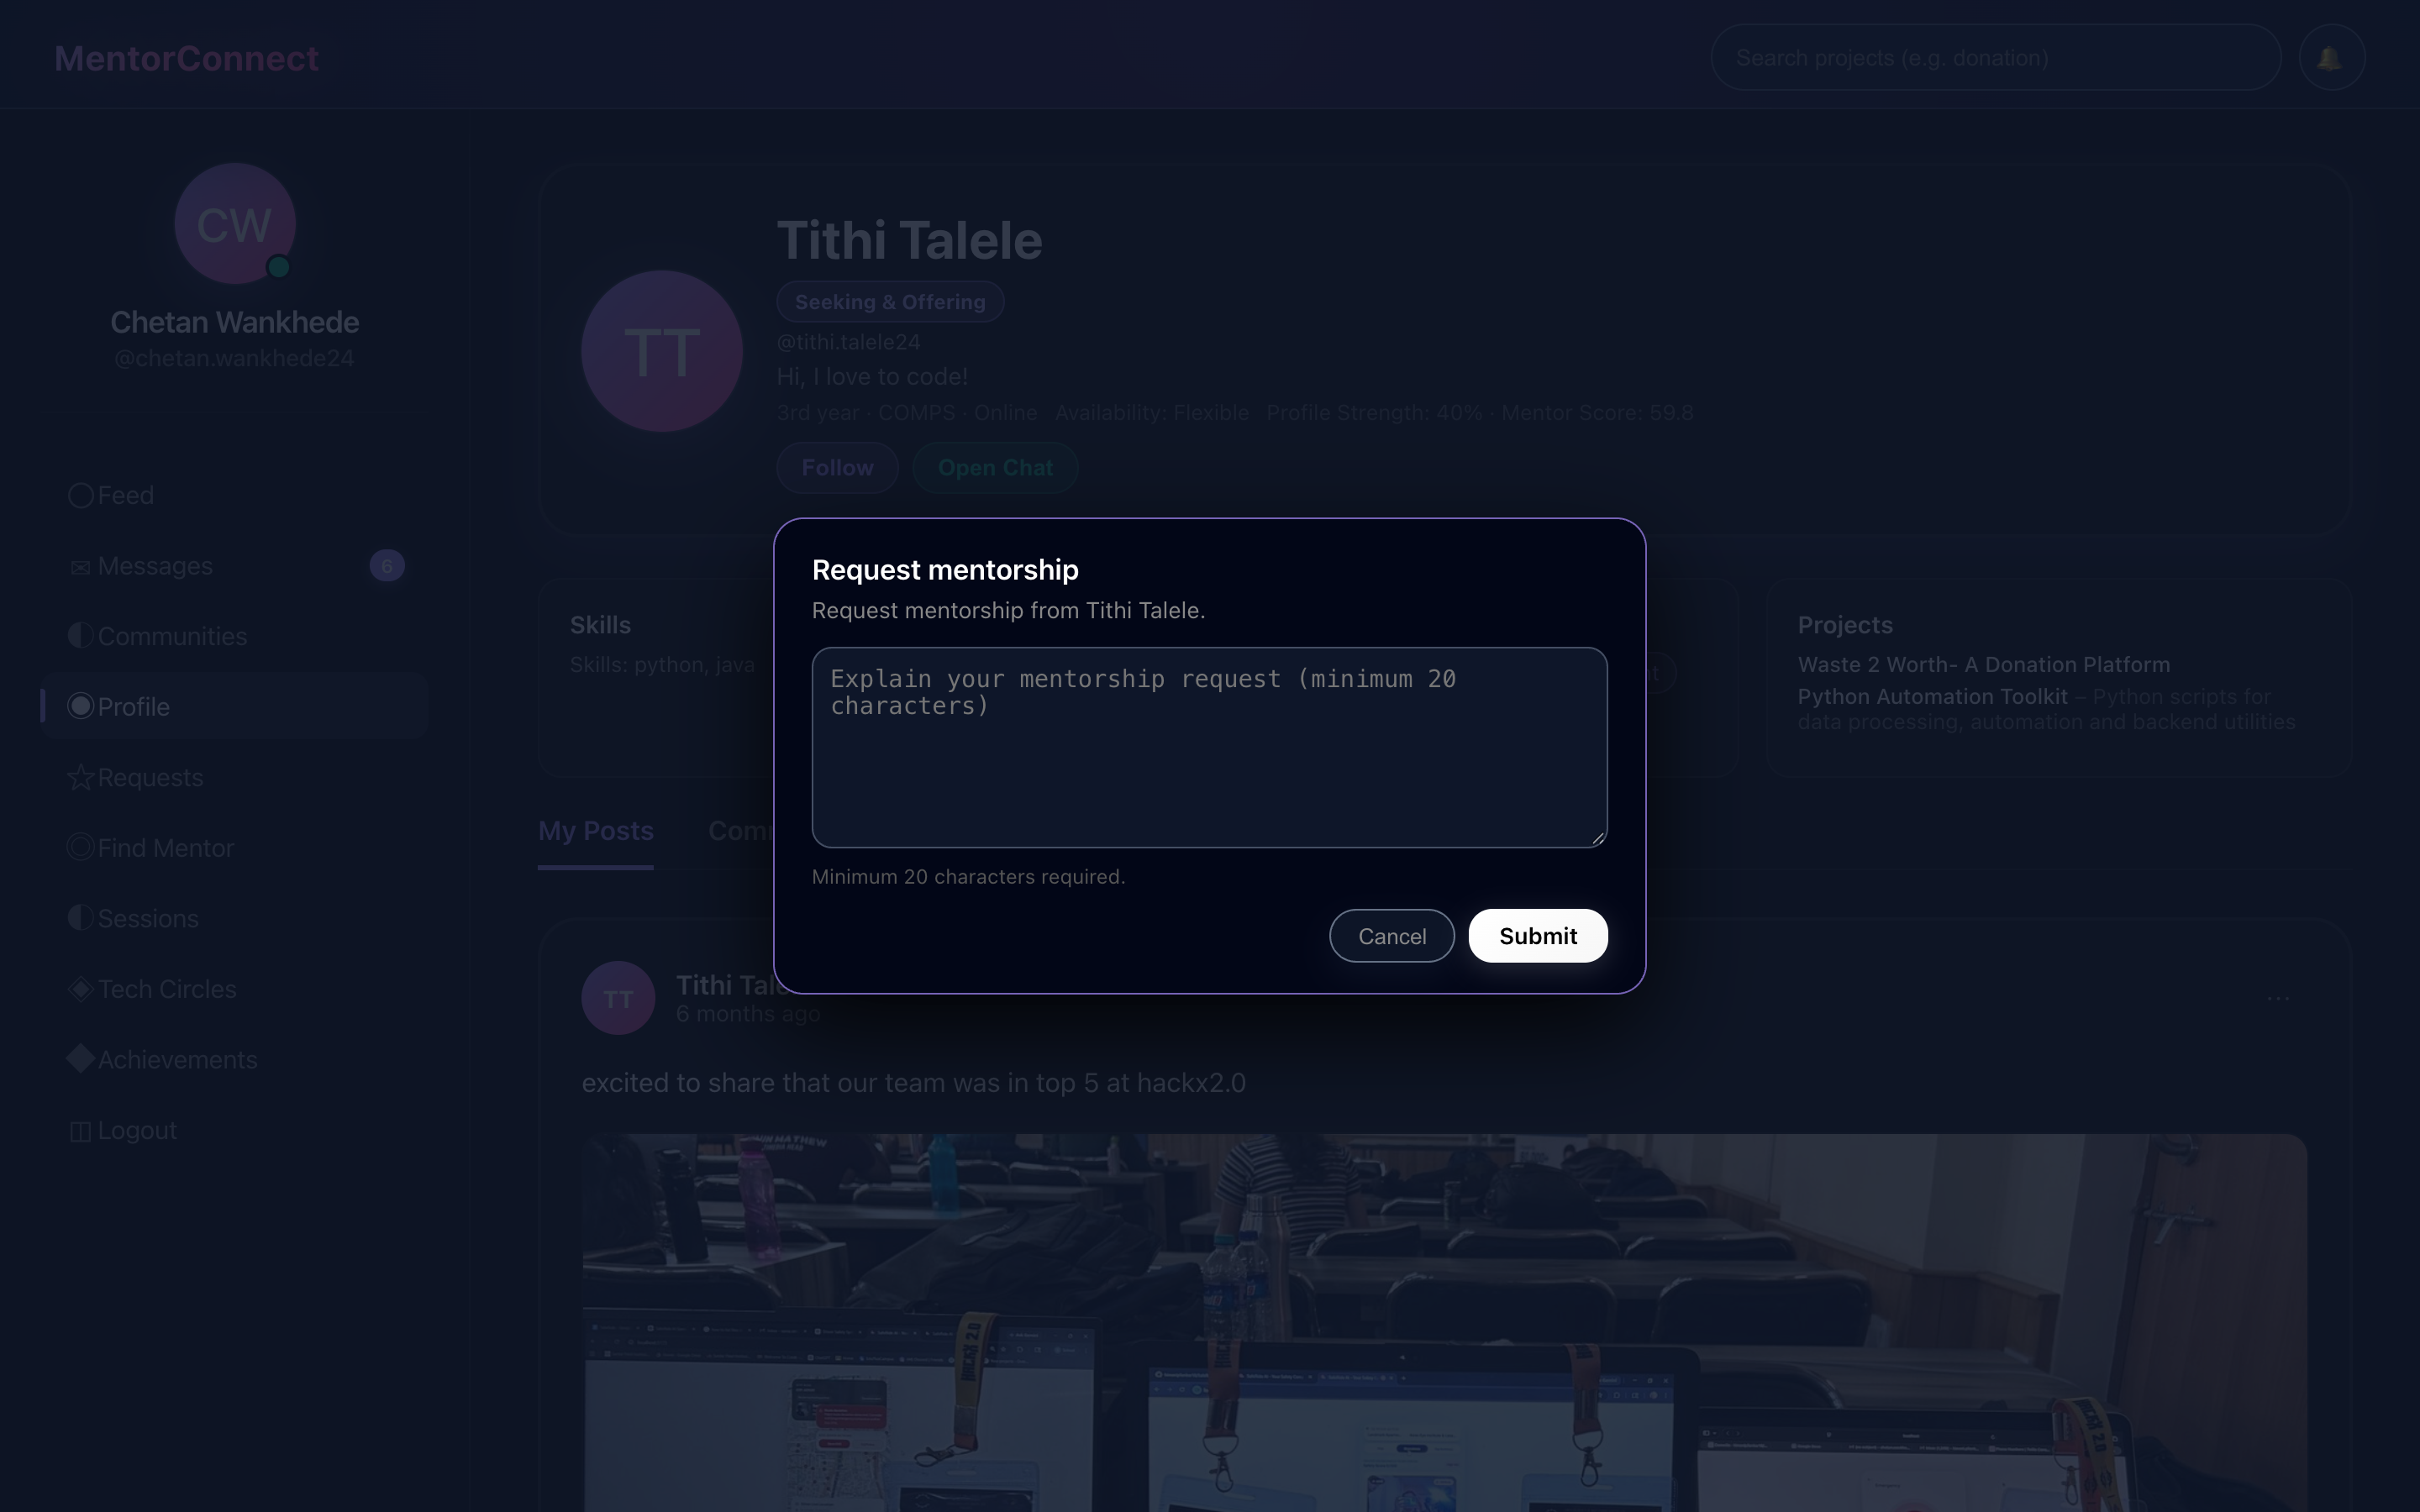
\includegraphics[width=0.95\textwidth]{figures/request-mentorship.png}
\caption{Sending a mentorship request with a short explanation}
\label{fig:ui-request}
\end{figure}

\begin{figure}[htbp]
\centering
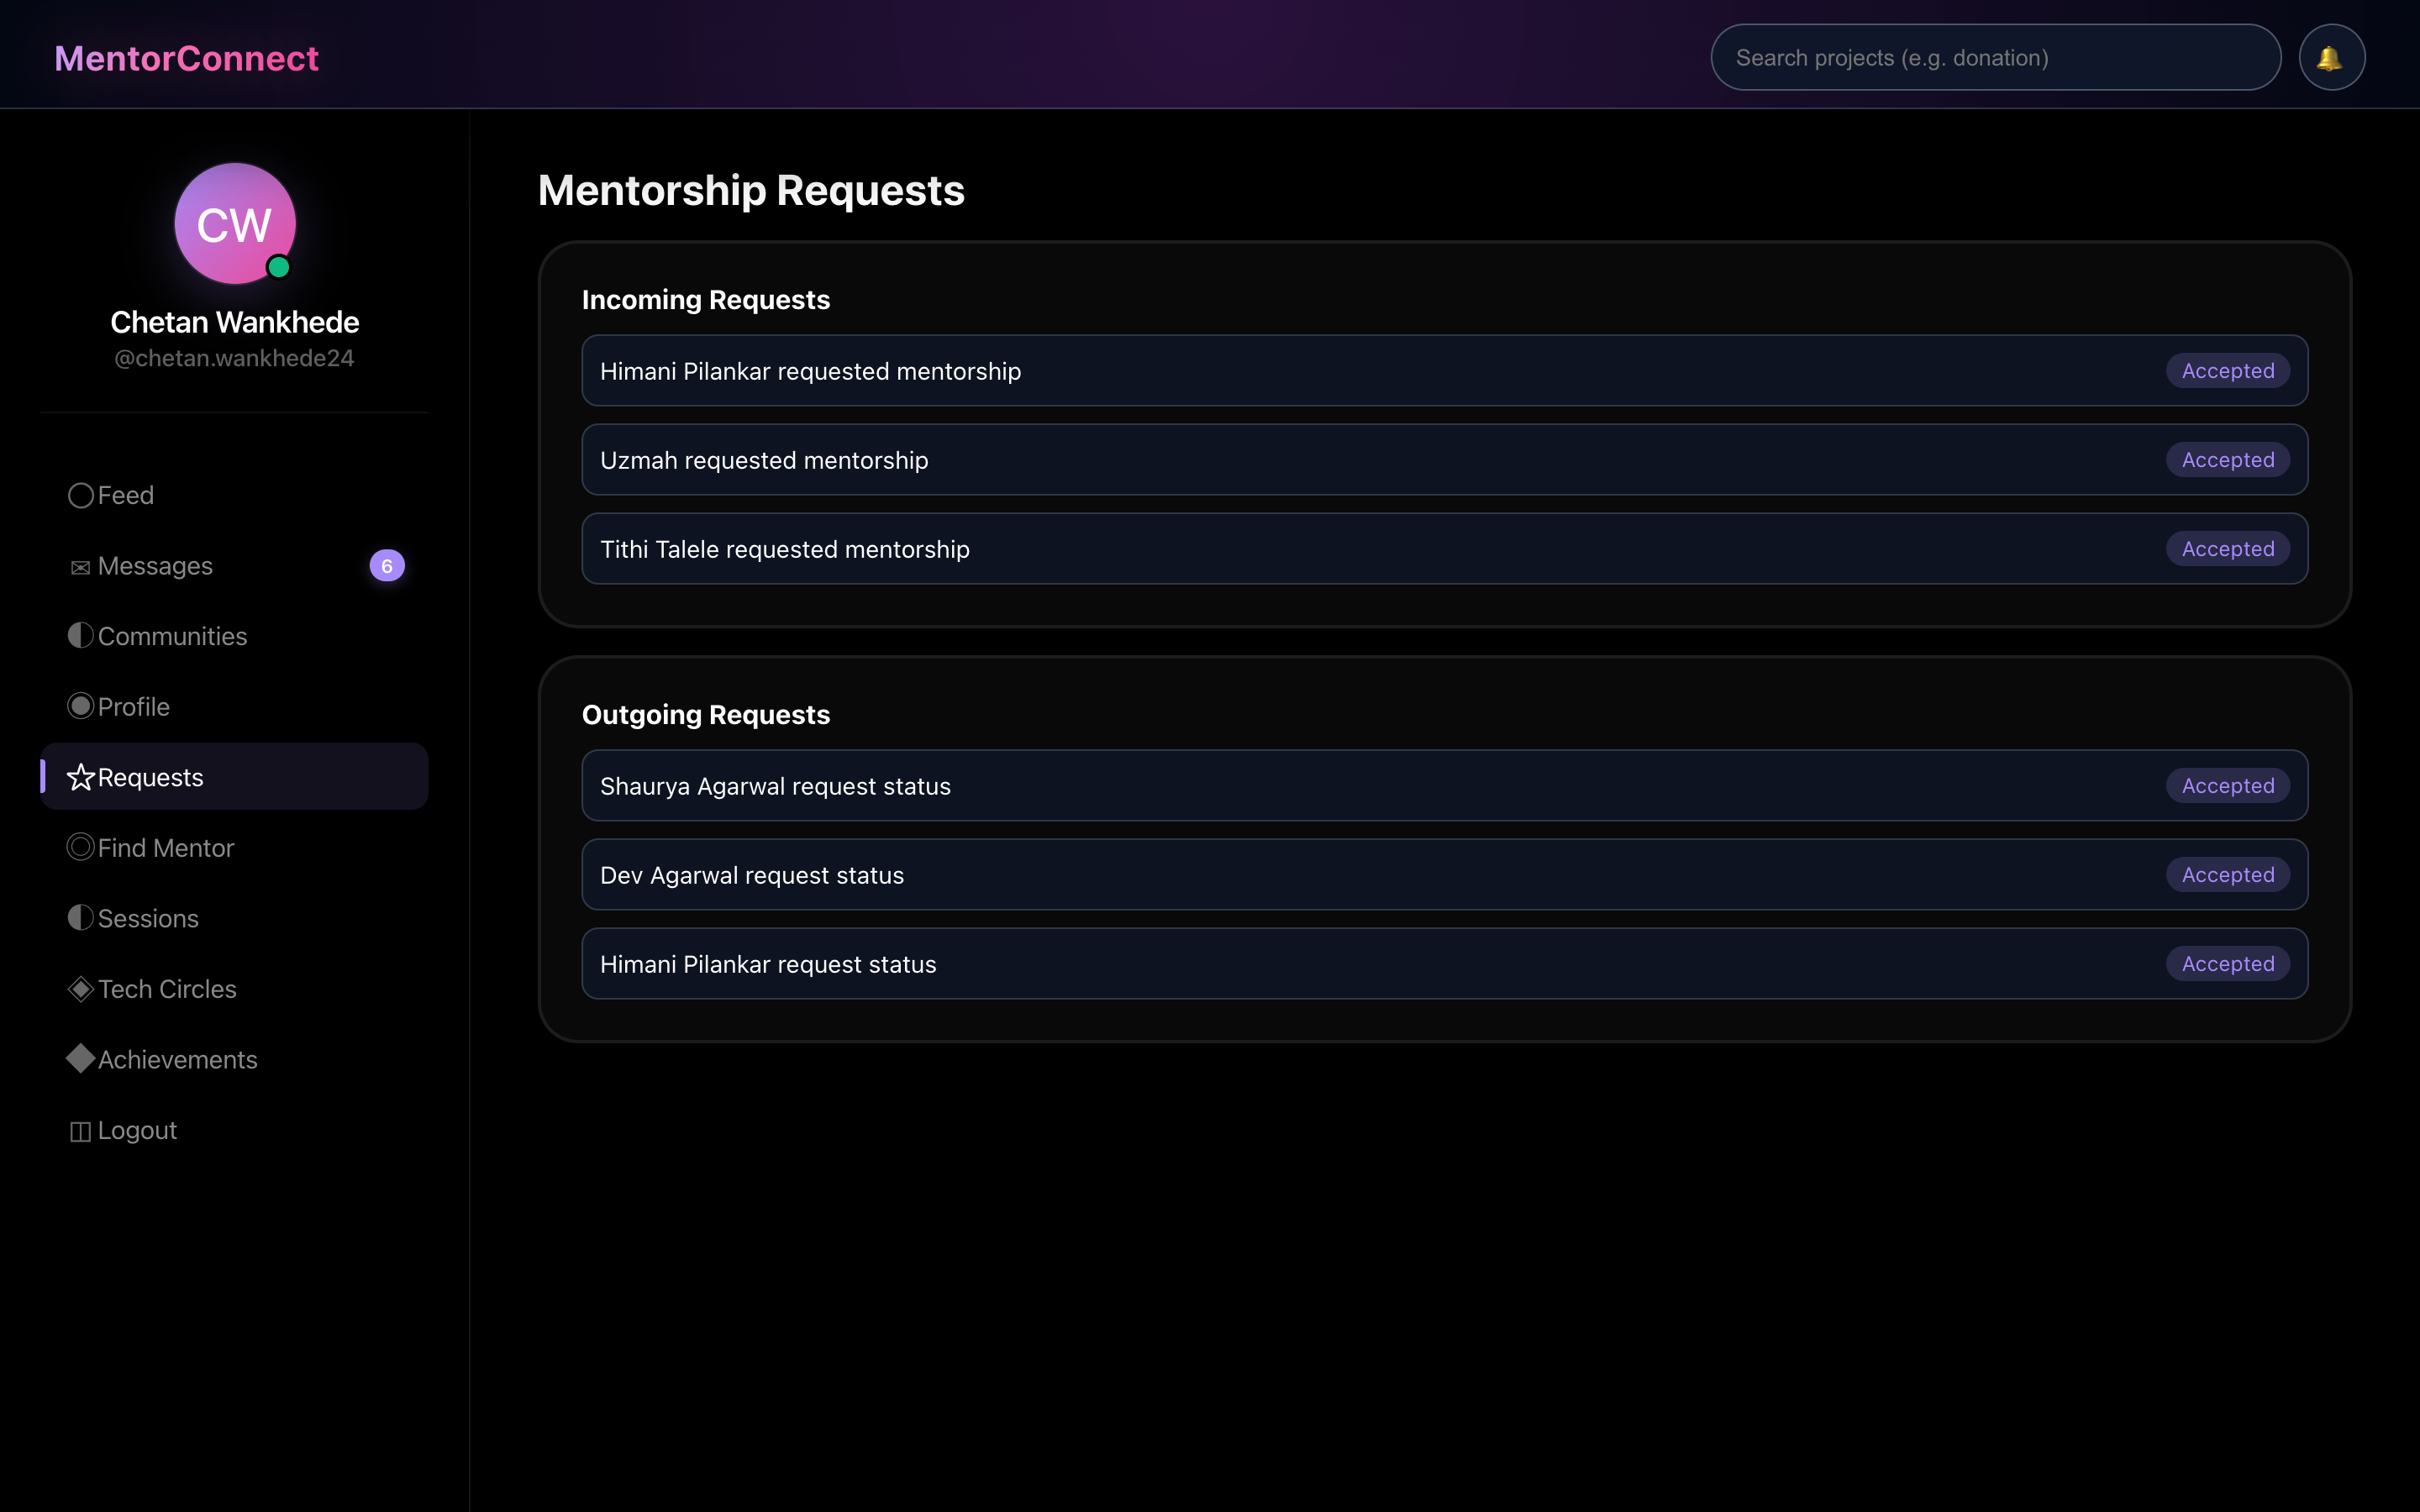
\includegraphics[width=0.95\textwidth]{figures/requests.png}
\caption{Mentorship requests received and sent, with their status}
\label{fig:ui-requests}
\end{figure}

A student requests mentorship by explaining what they need help with in at least twenty characters (Figure~\ref{fig:ui-request}). The Requests page (Figure~\ref{fig:ui-requests}) shows incoming and outgoing requests with their status; a mentor can accept or decline each incoming request, and accepting one opens a private chat for the pair.

\subsection{Messages}
\begin{figure}[htbp]
\centering
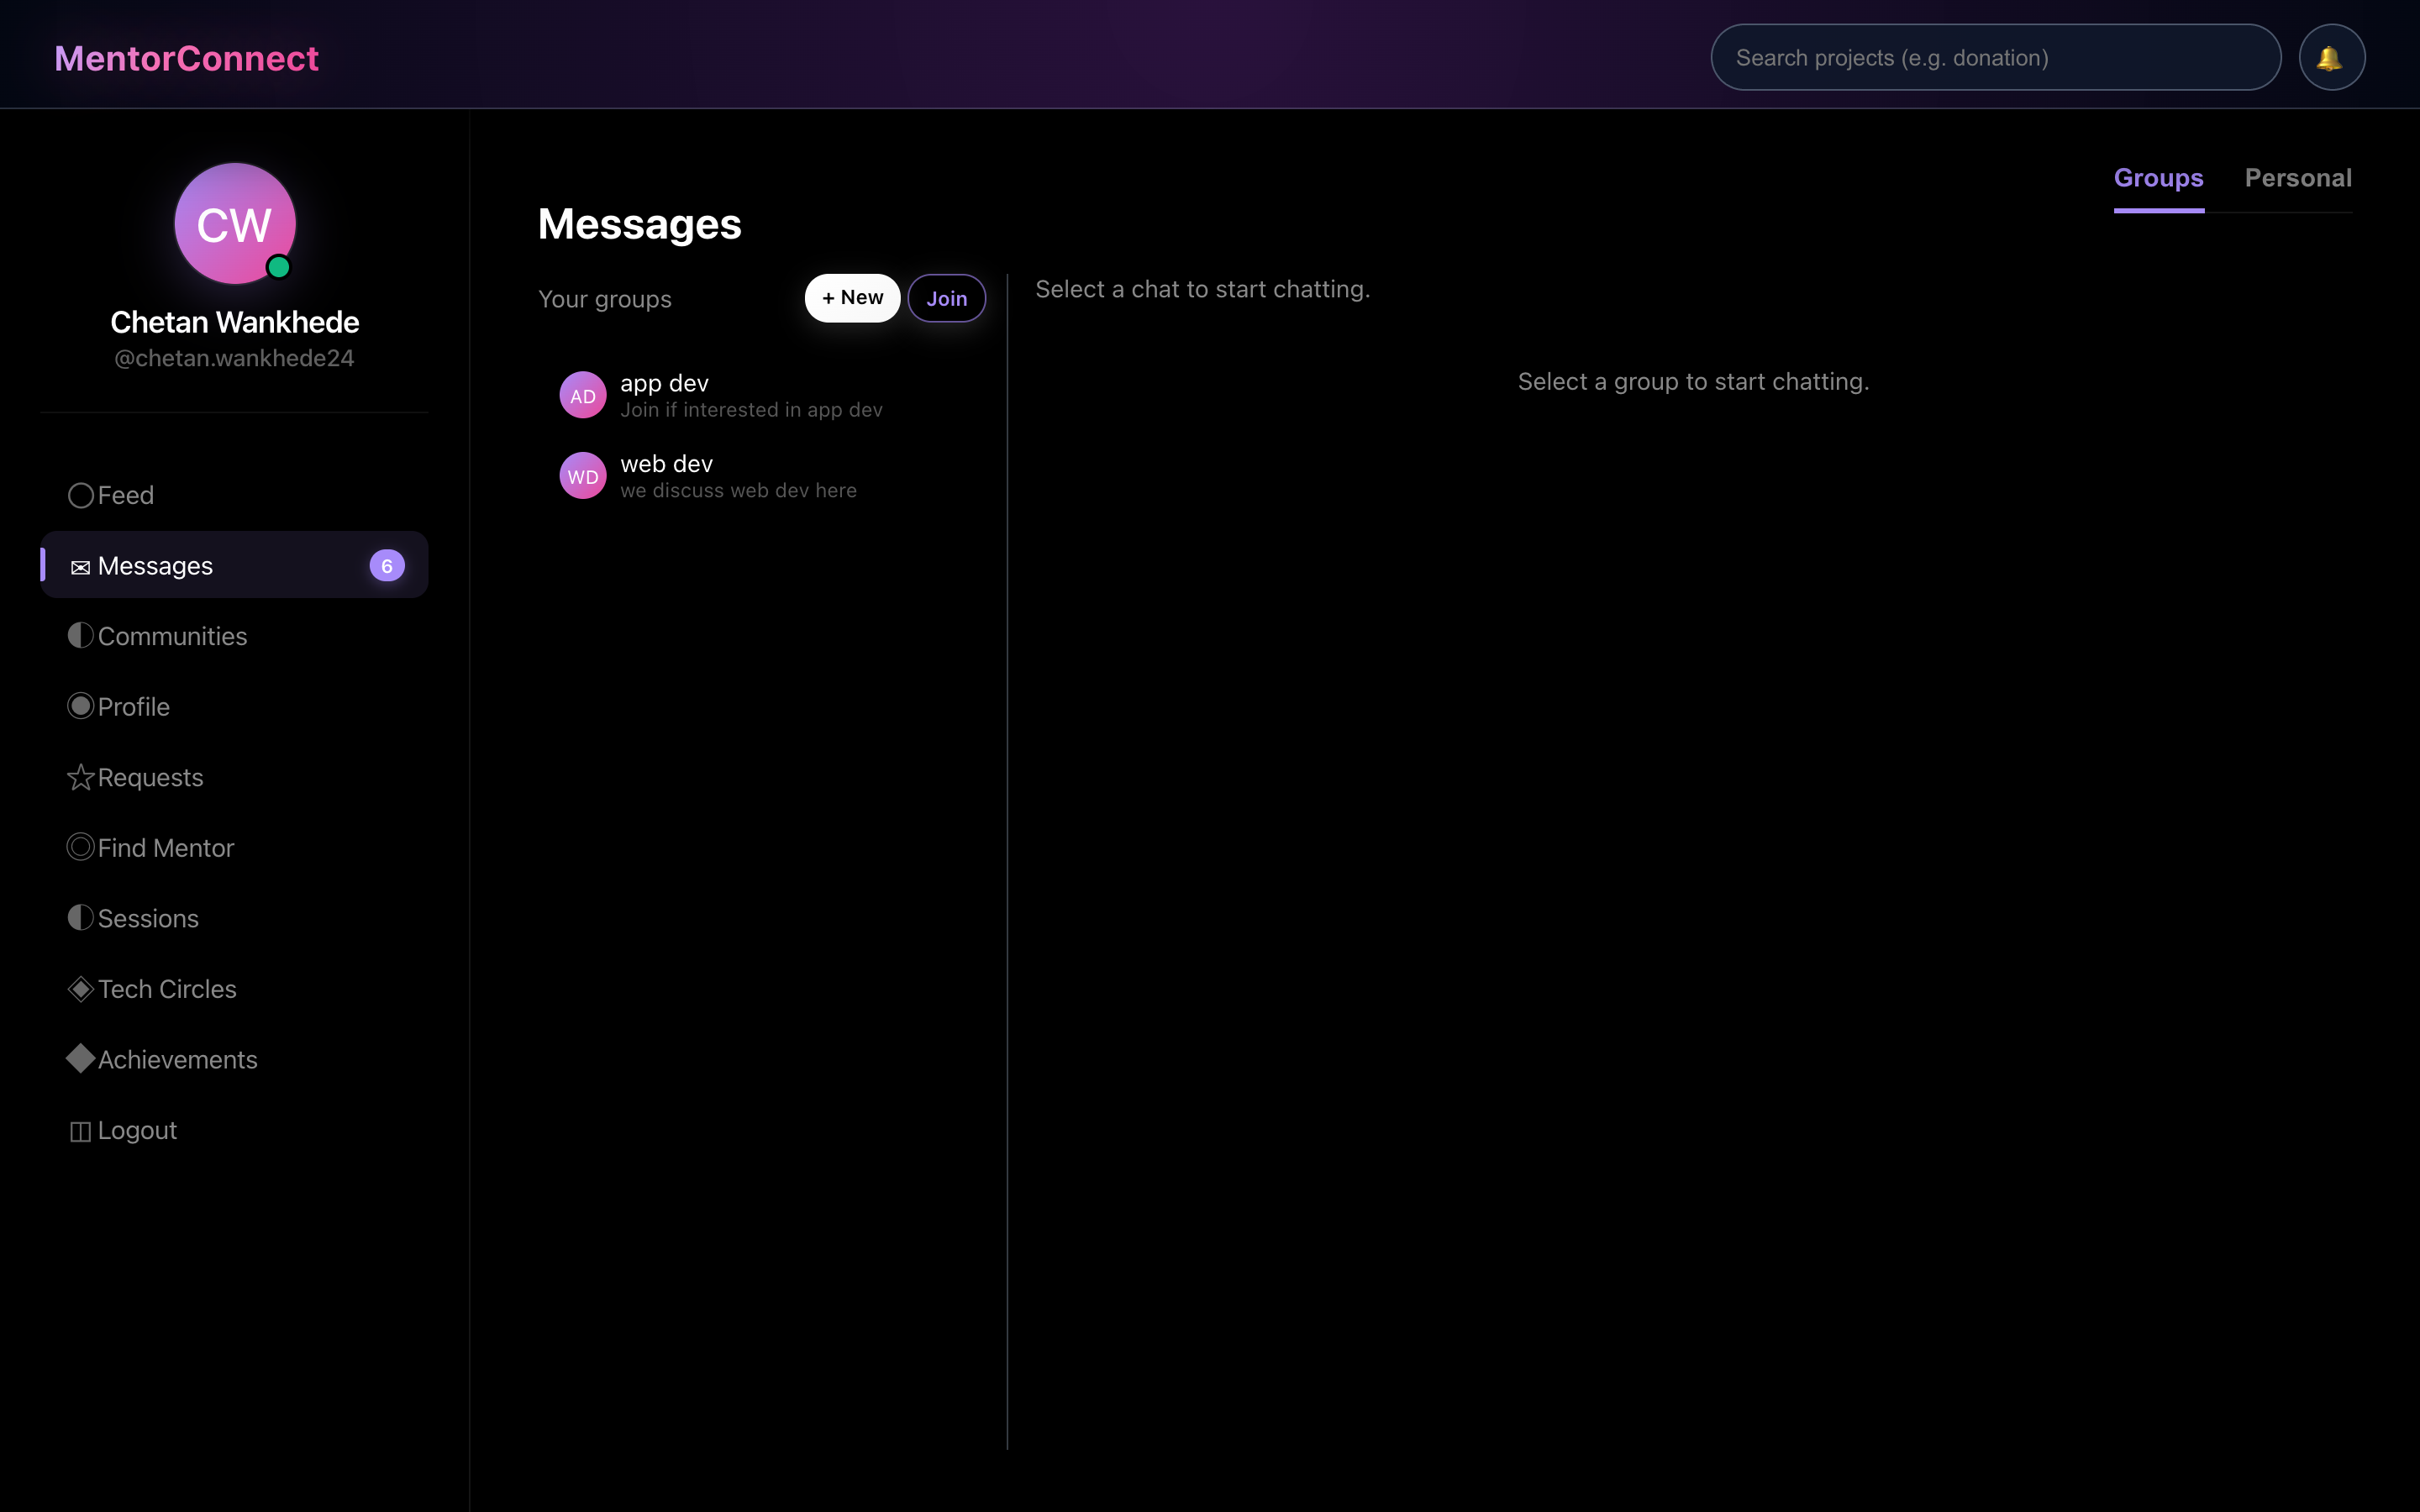
\includegraphics[width=0.95\textwidth]{figures/messages.png}
\caption{Messages: the student's chat groups}
\label{fig:ui-messages}
\end{figure}

\begin{figure}[htbp]
\centering
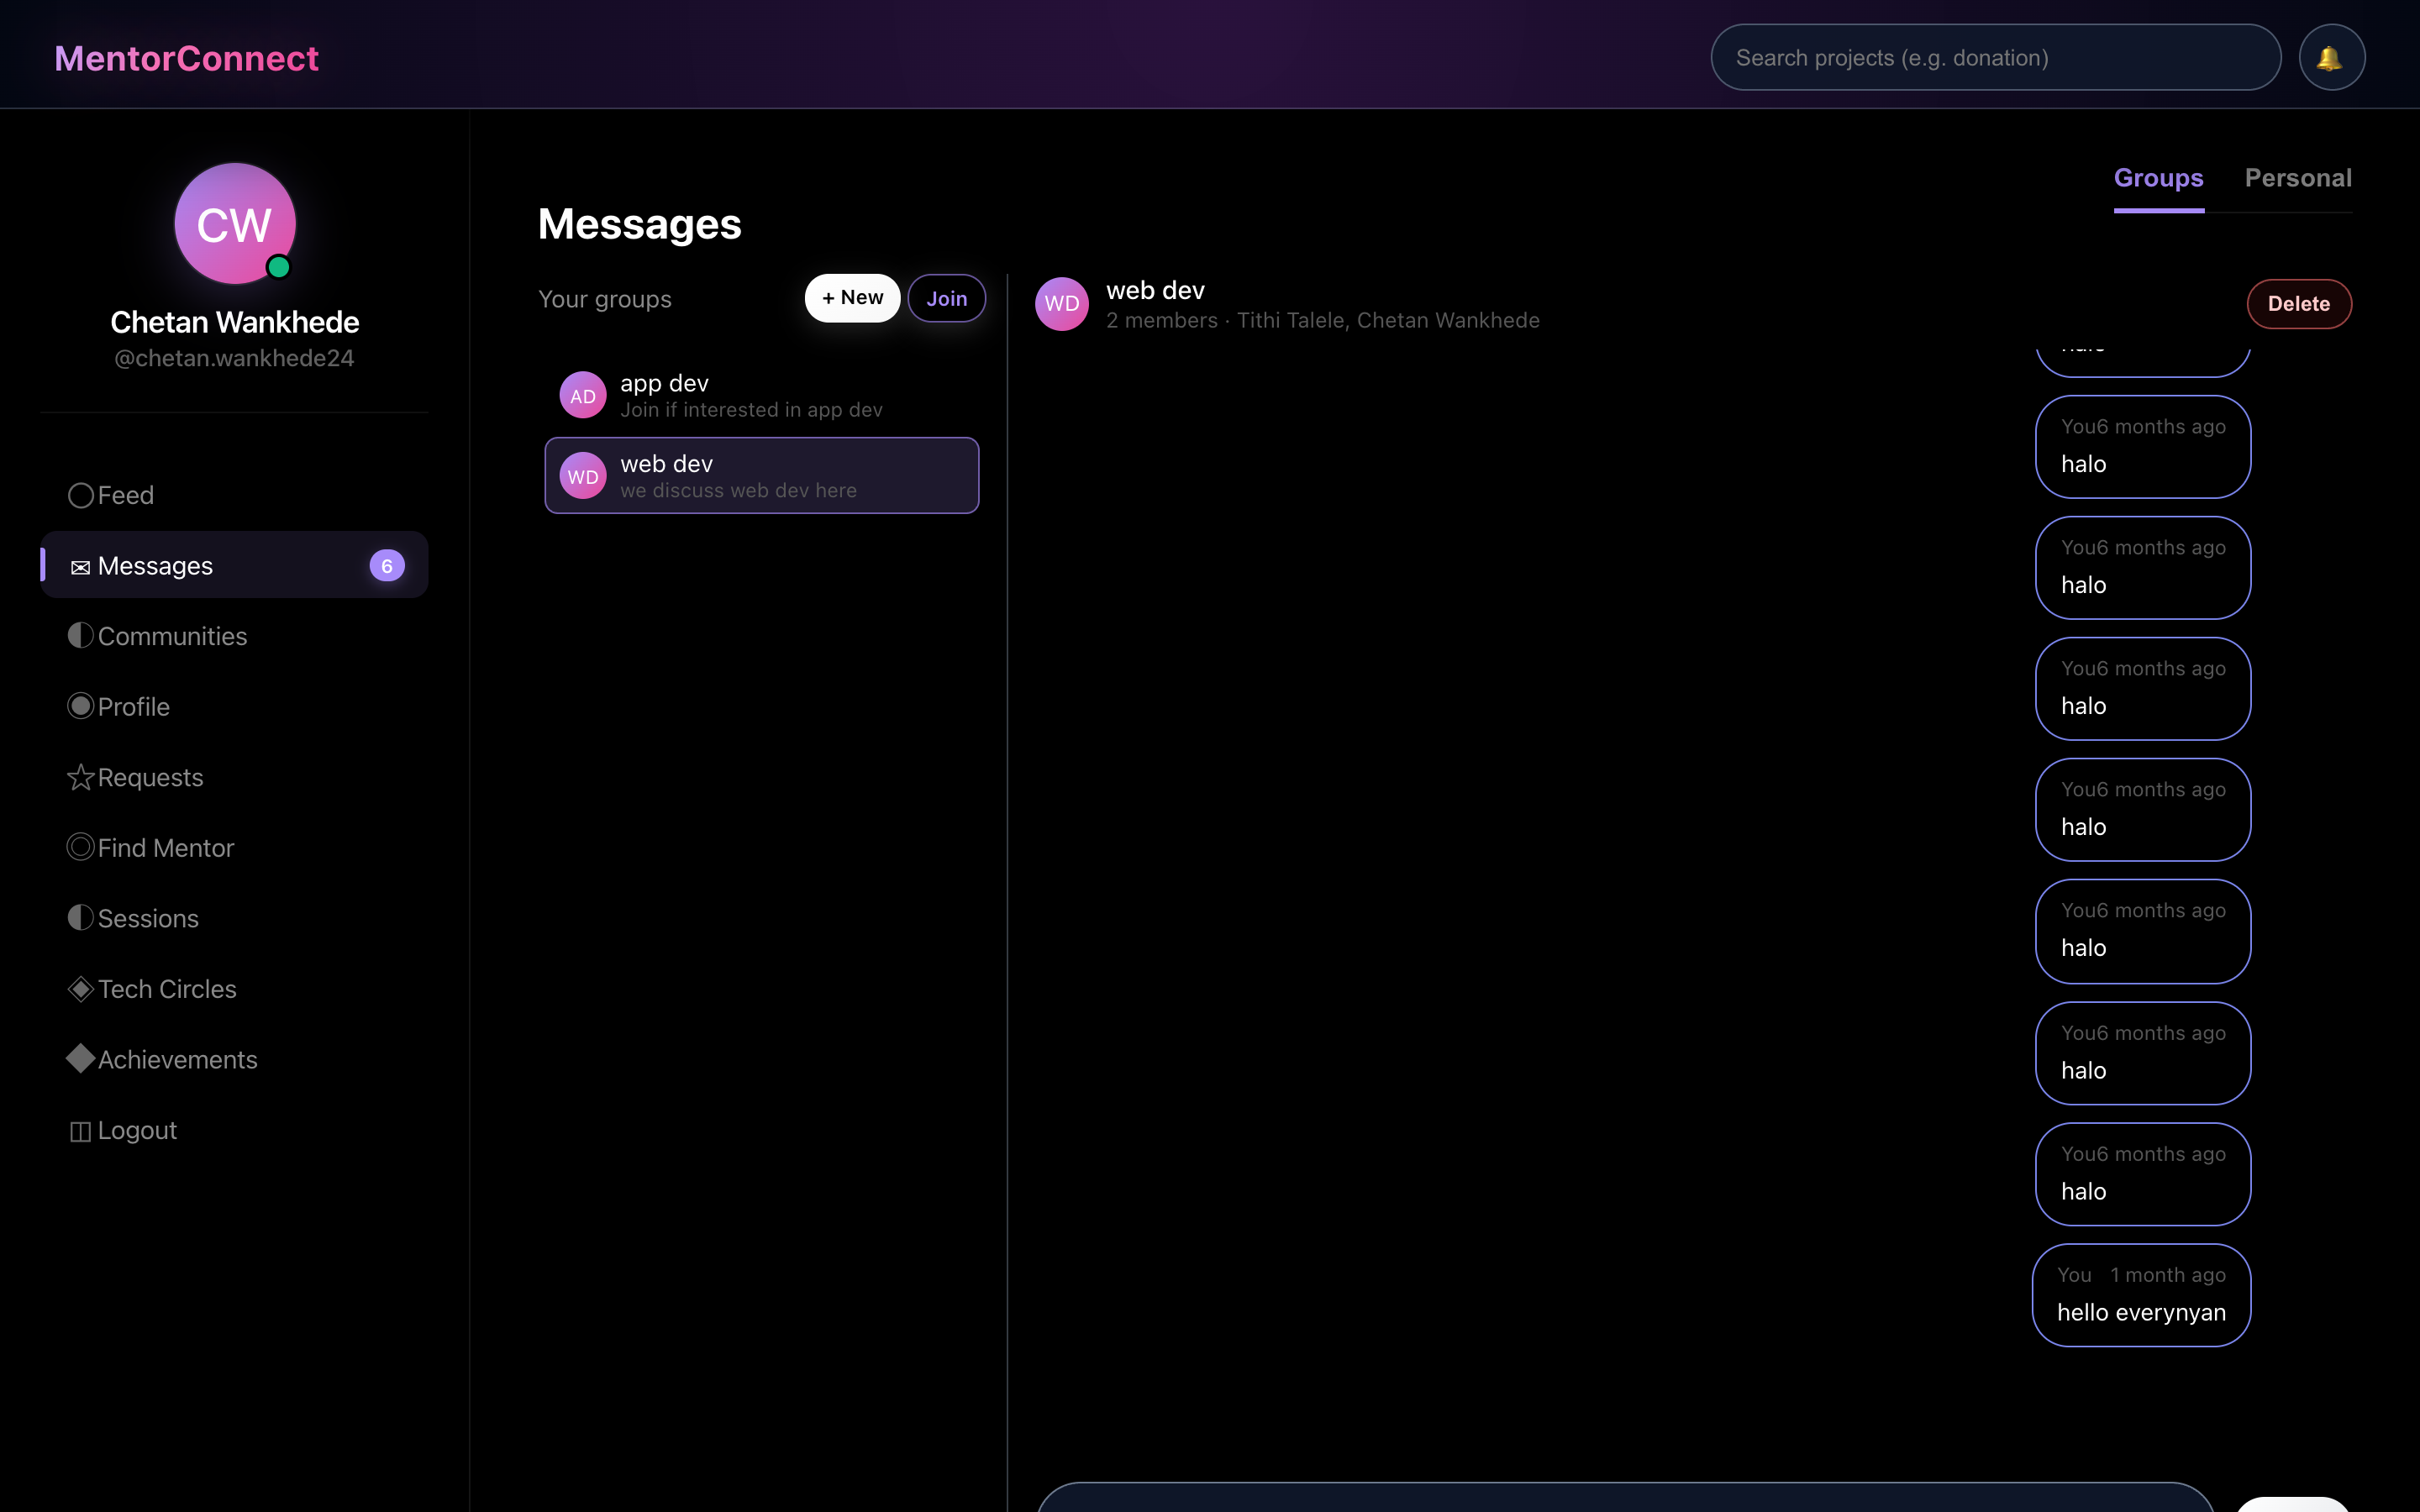
\includegraphics[width=0.95\textwidth]{figures/messages-chat.png}
\caption{A group conversation}
\label{fig:ui-messages-chat}
\end{figure}

\begin{figure}[htbp]
\centering
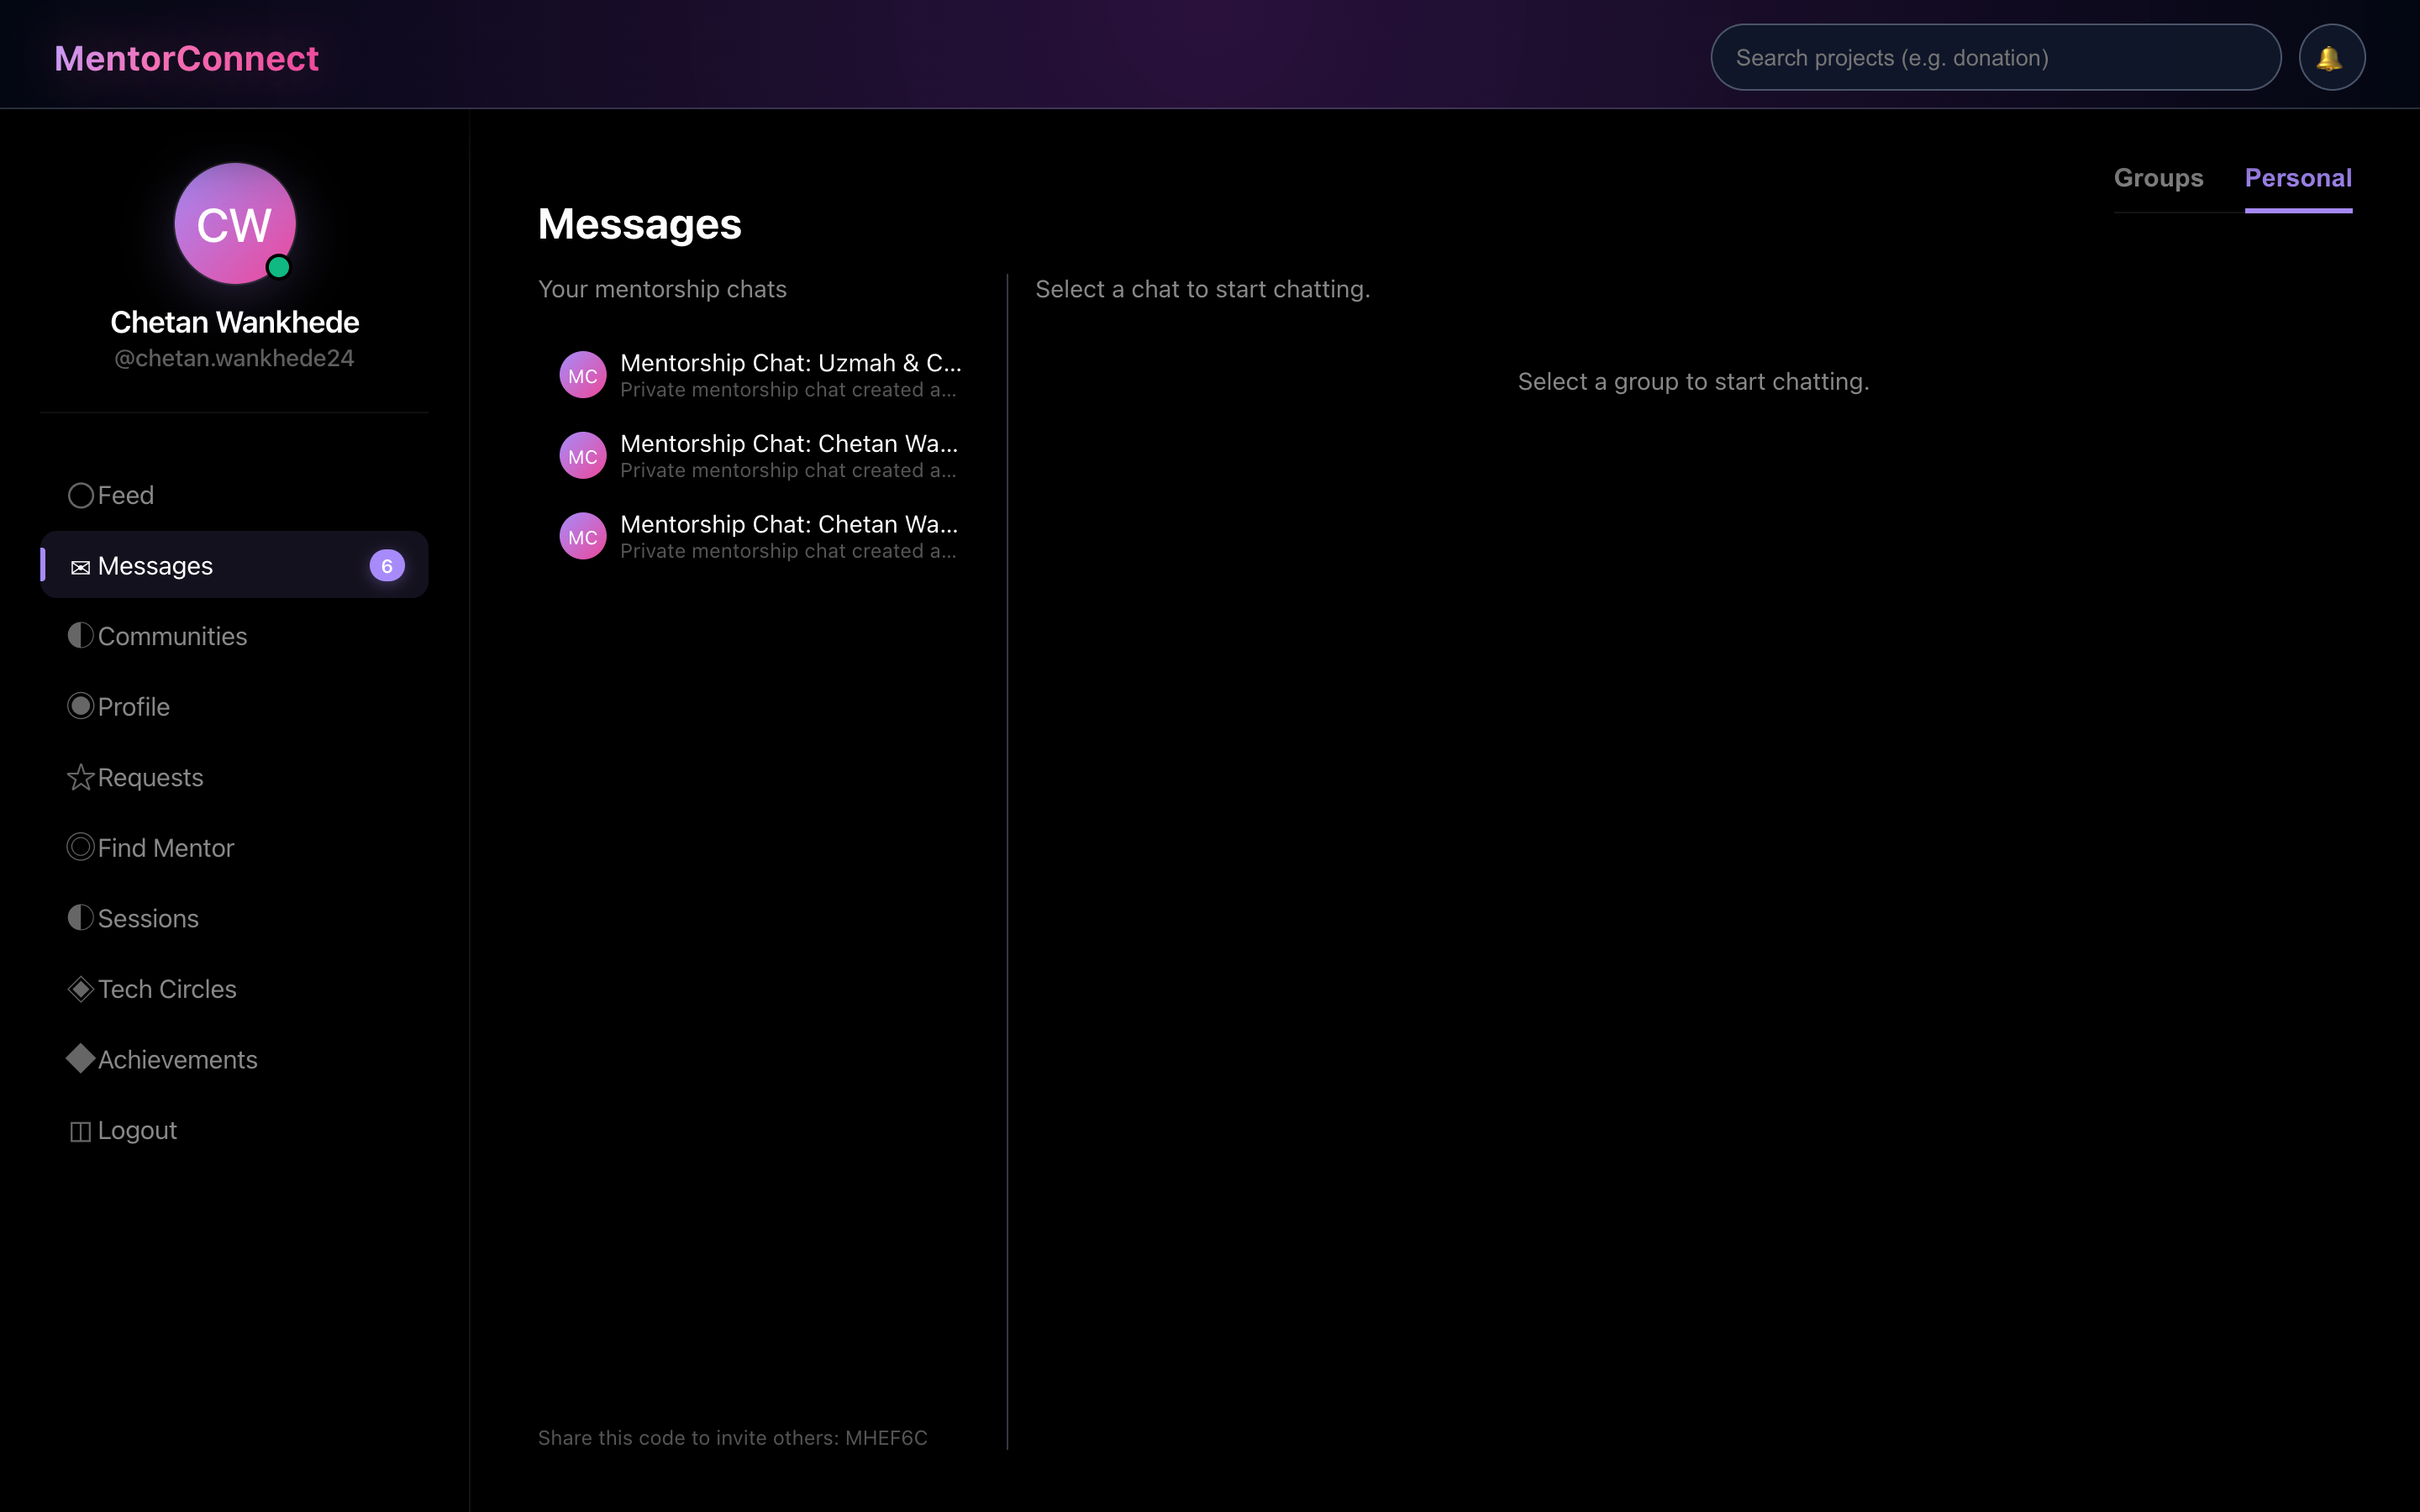
\includegraphics[width=0.95\textwidth]{figures/messages-personal.png}
\caption{Private mentorship chats created when requests are accepted}
\label{fig:ui-messages-personal}
\end{figure}

\begin{figure}[htbp]
\centering
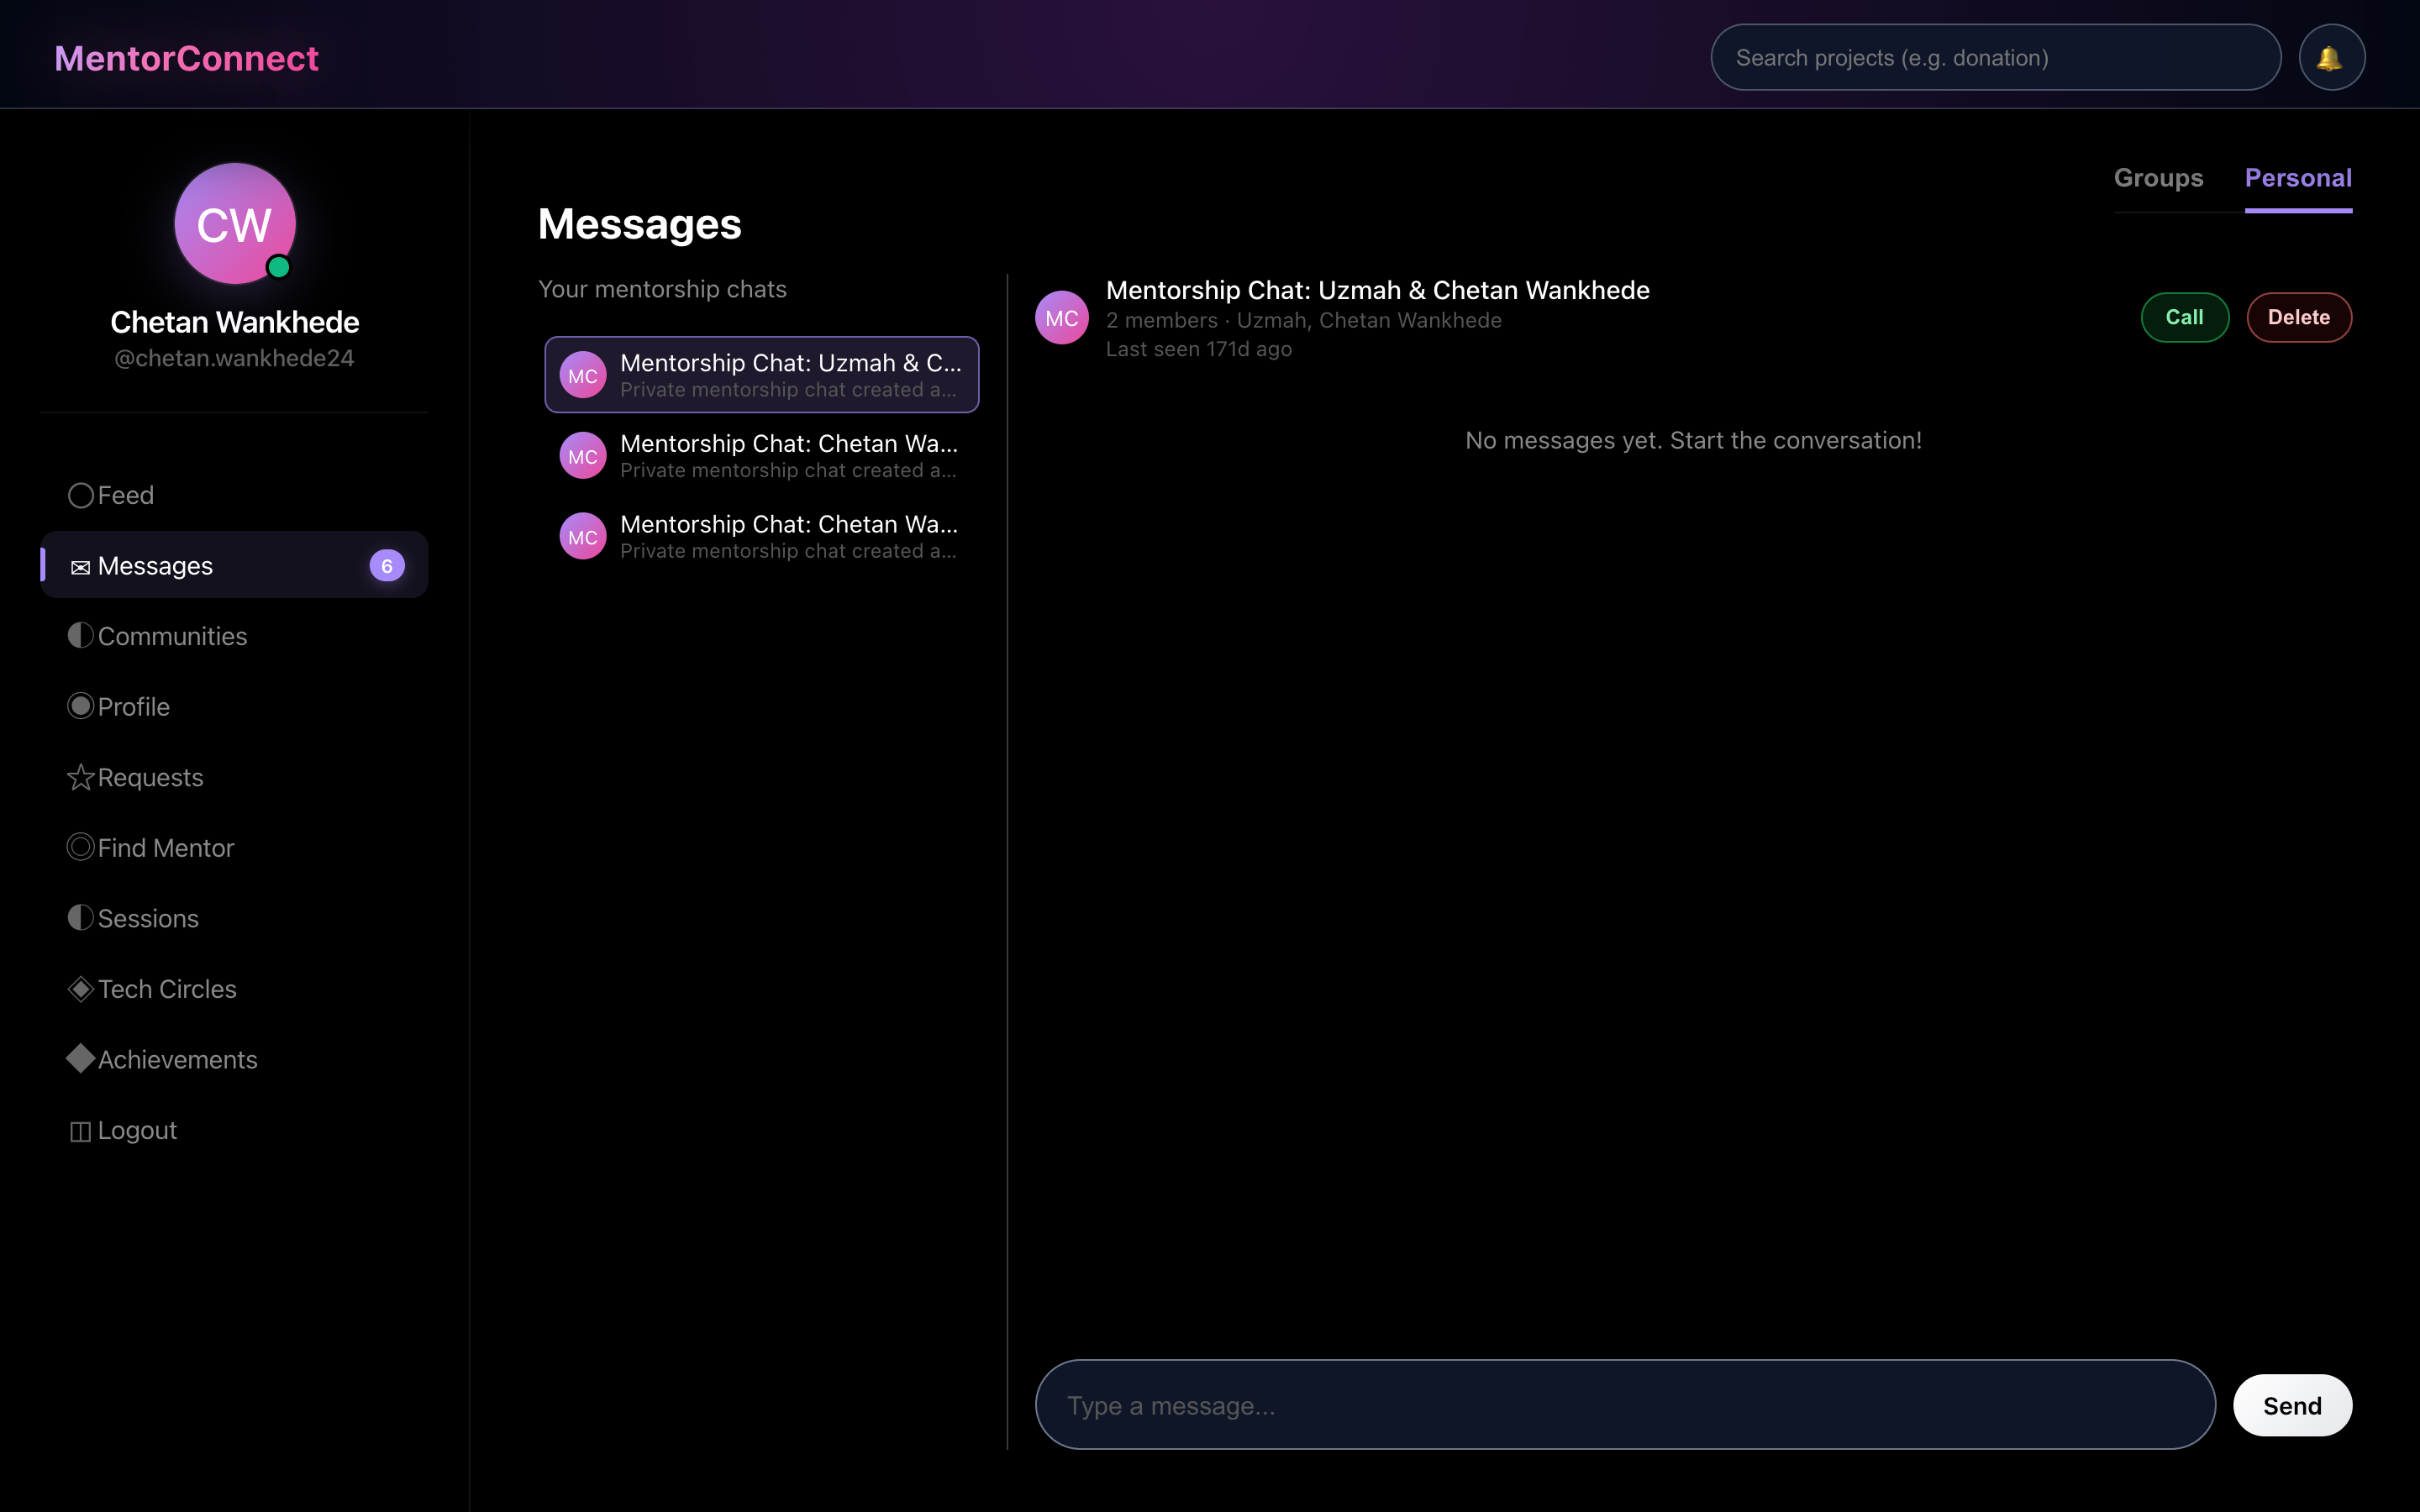
\includegraphics[width=0.95\textwidth]{figures/messages-personal-chat.png}
\caption{A newly created mentorship chat with its call option}
\label{fig:ui-messages-new}
\end{figure}

\begin{figure}[htbp]
\centering
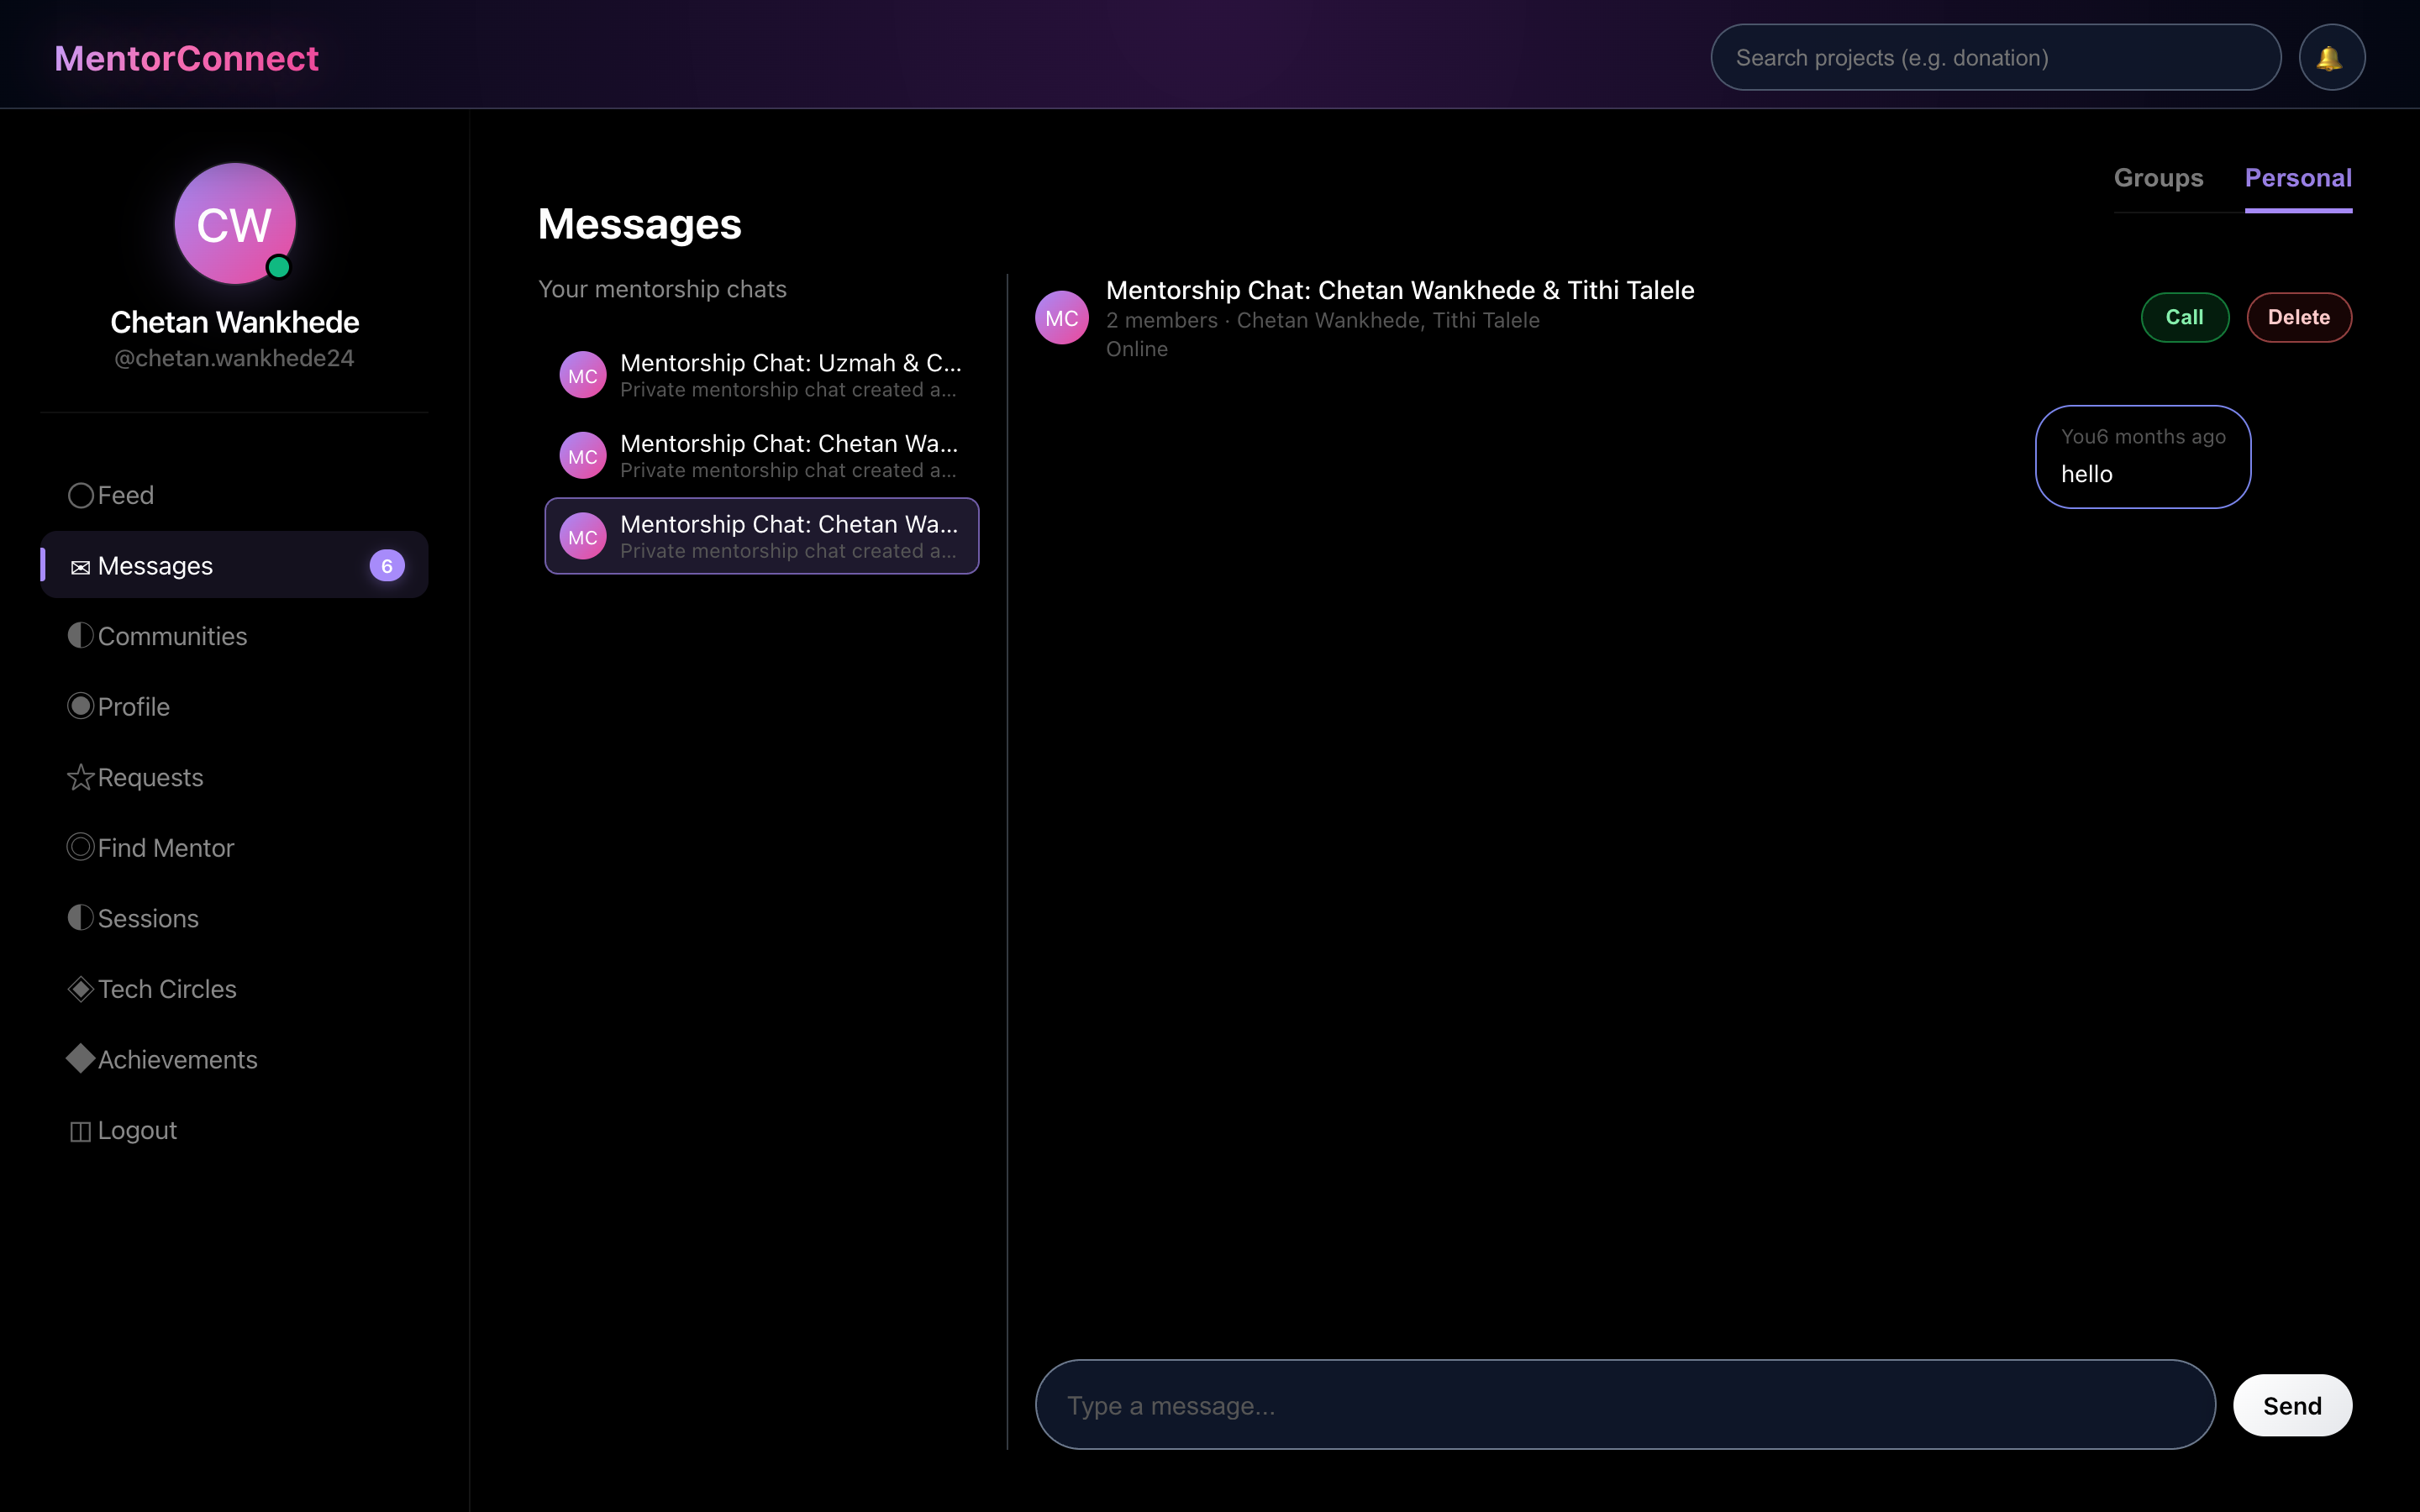
\includegraphics[width=0.95\textwidth]{figures/messages-mentorship-chat.png}
\caption{A mentorship conversation between a mentor and mentee}
\label{fig:ui-messages-mentorship}
\end{figure}

Messages has two tabs. Groups (Figures~\ref{fig:ui-messages} and~\ref{fig:ui-messages-chat}) are topic chats that students create or join with an invite code. Personal chats (Figures~\ref{fig:ui-messages-personal}--\ref{fig:ui-messages-mentorship}) are the private mentorship chats created automatically when a mentorship request is accepted; they show each participant's online status and offer a call option. Messages are delivered in real time through Socket.IO.

\subsection{Communities and Tech Circles}
\begin{figure}[htbp]
\centering
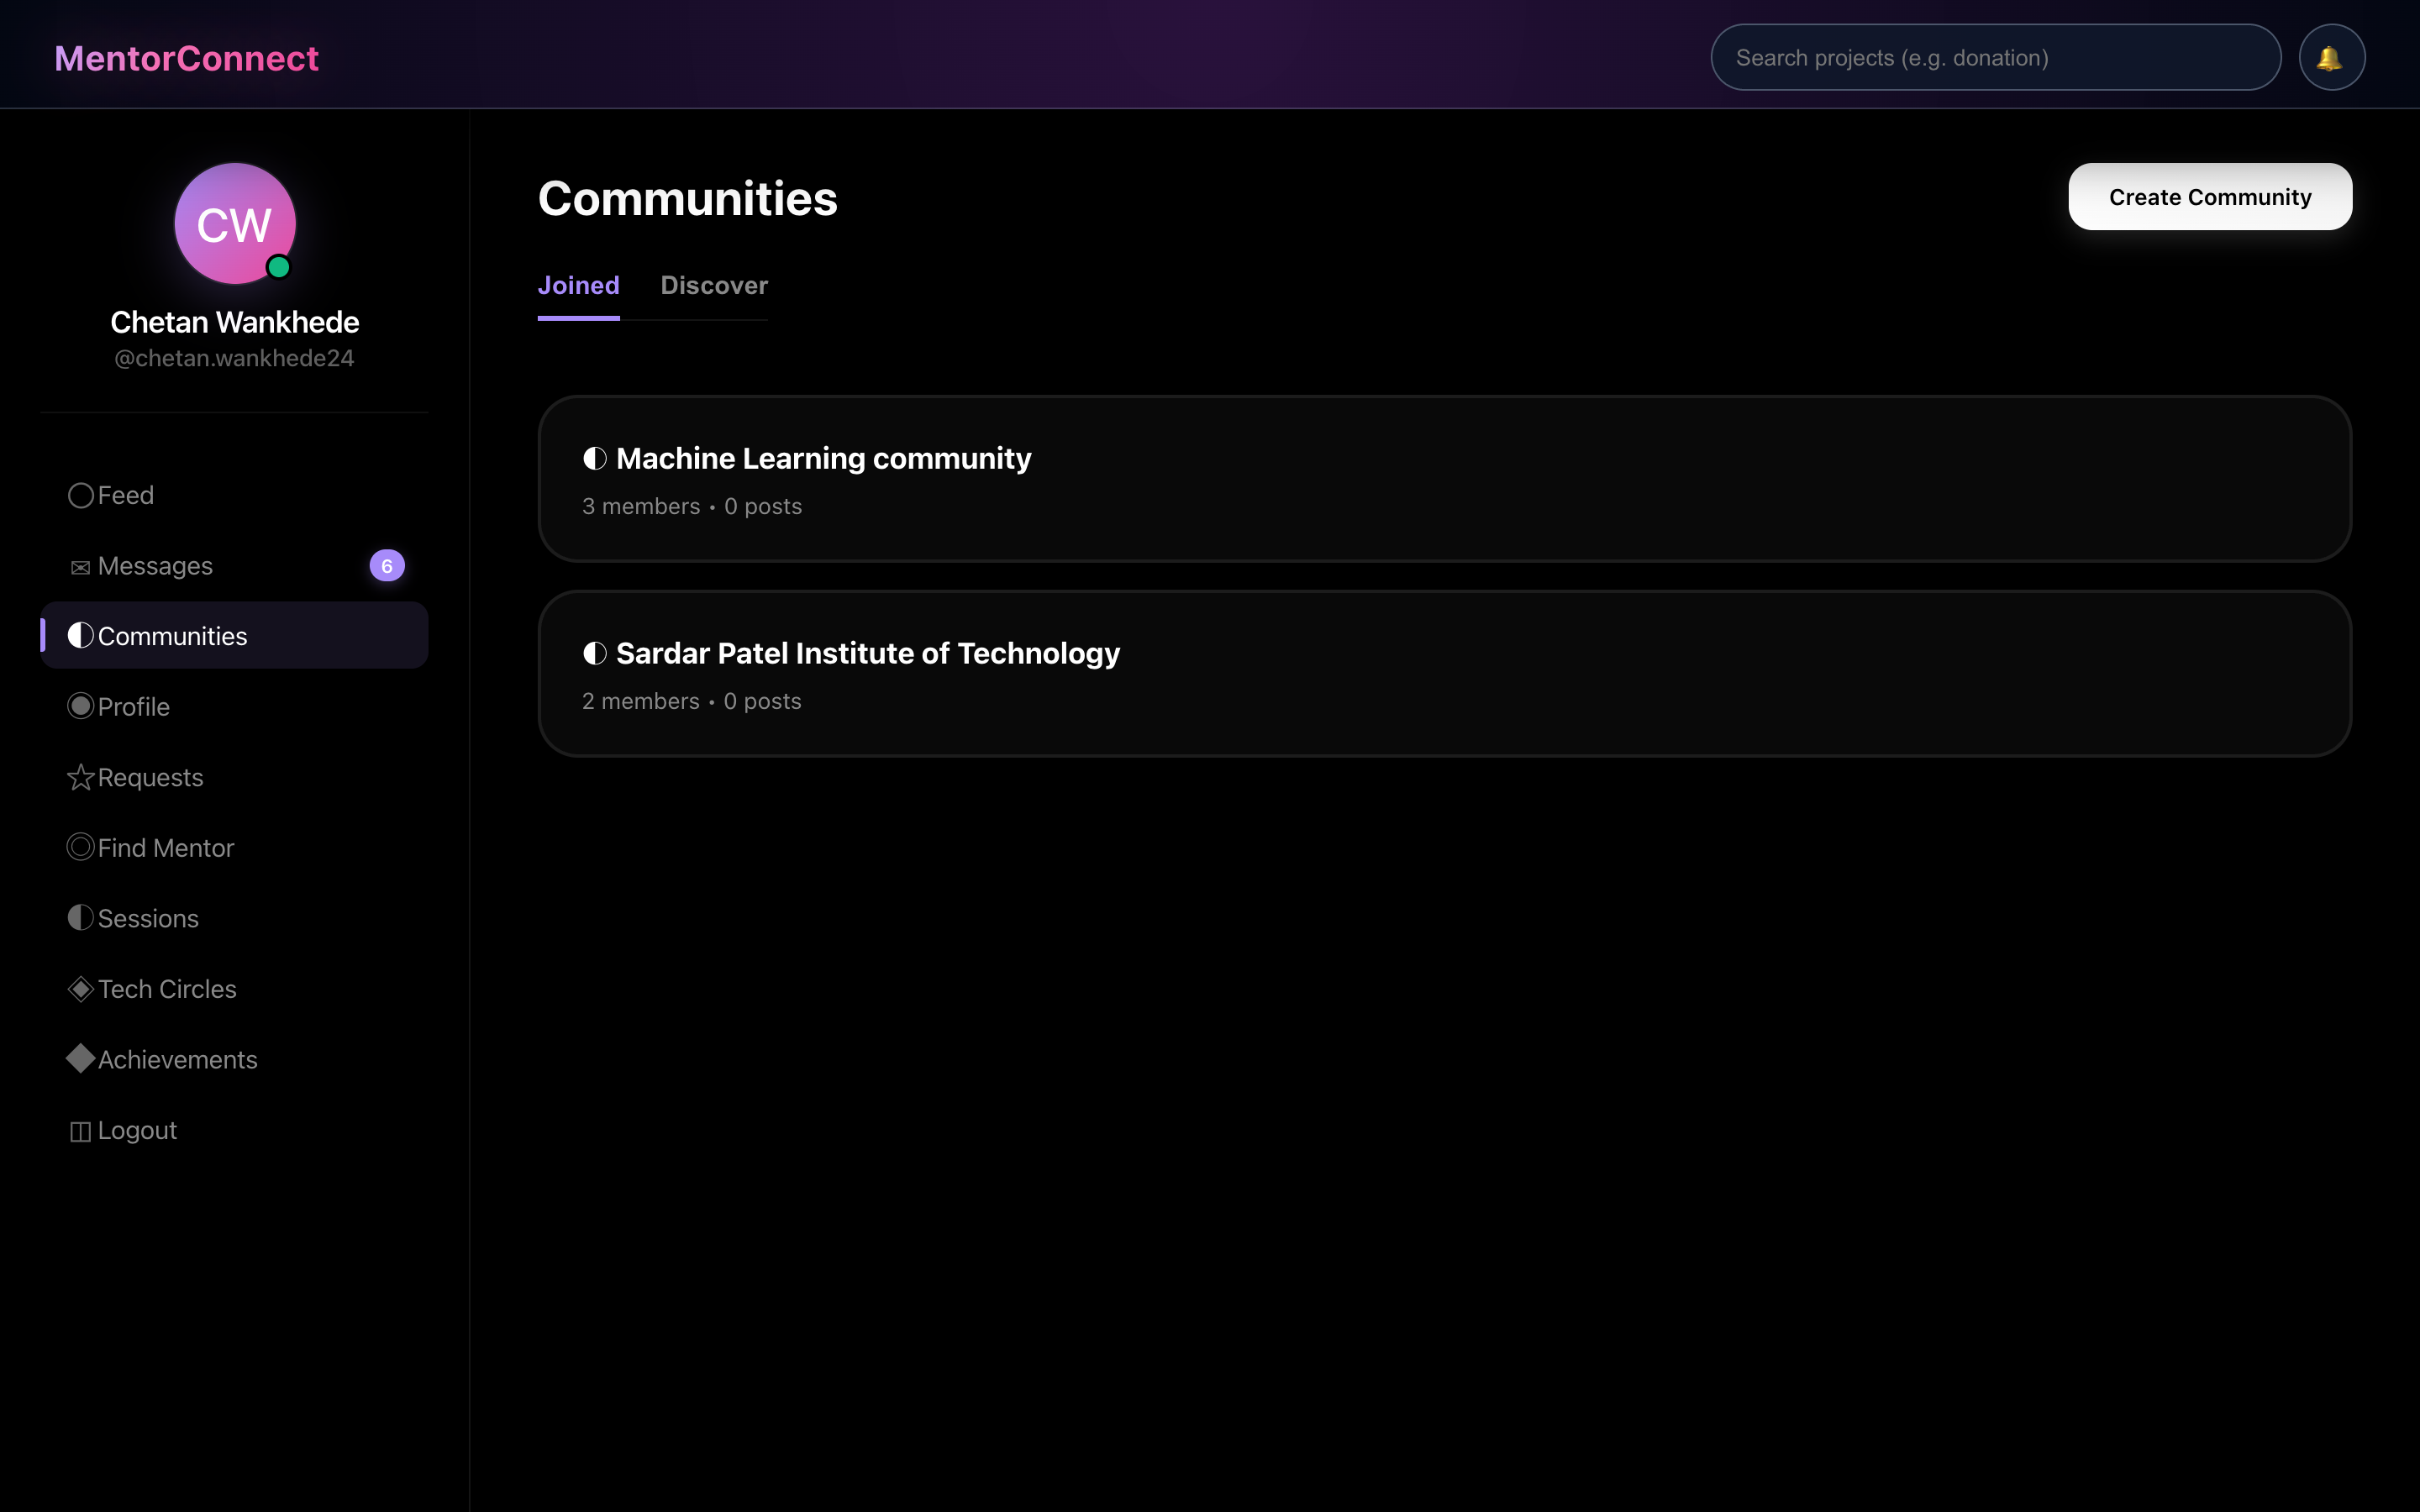
\includegraphics[width=0.95\textwidth]{figures/communities.png}
\caption{Communities joined by the student}
\label{fig:ui-communities}
\end{figure}

\begin{figure}[htbp]
\centering
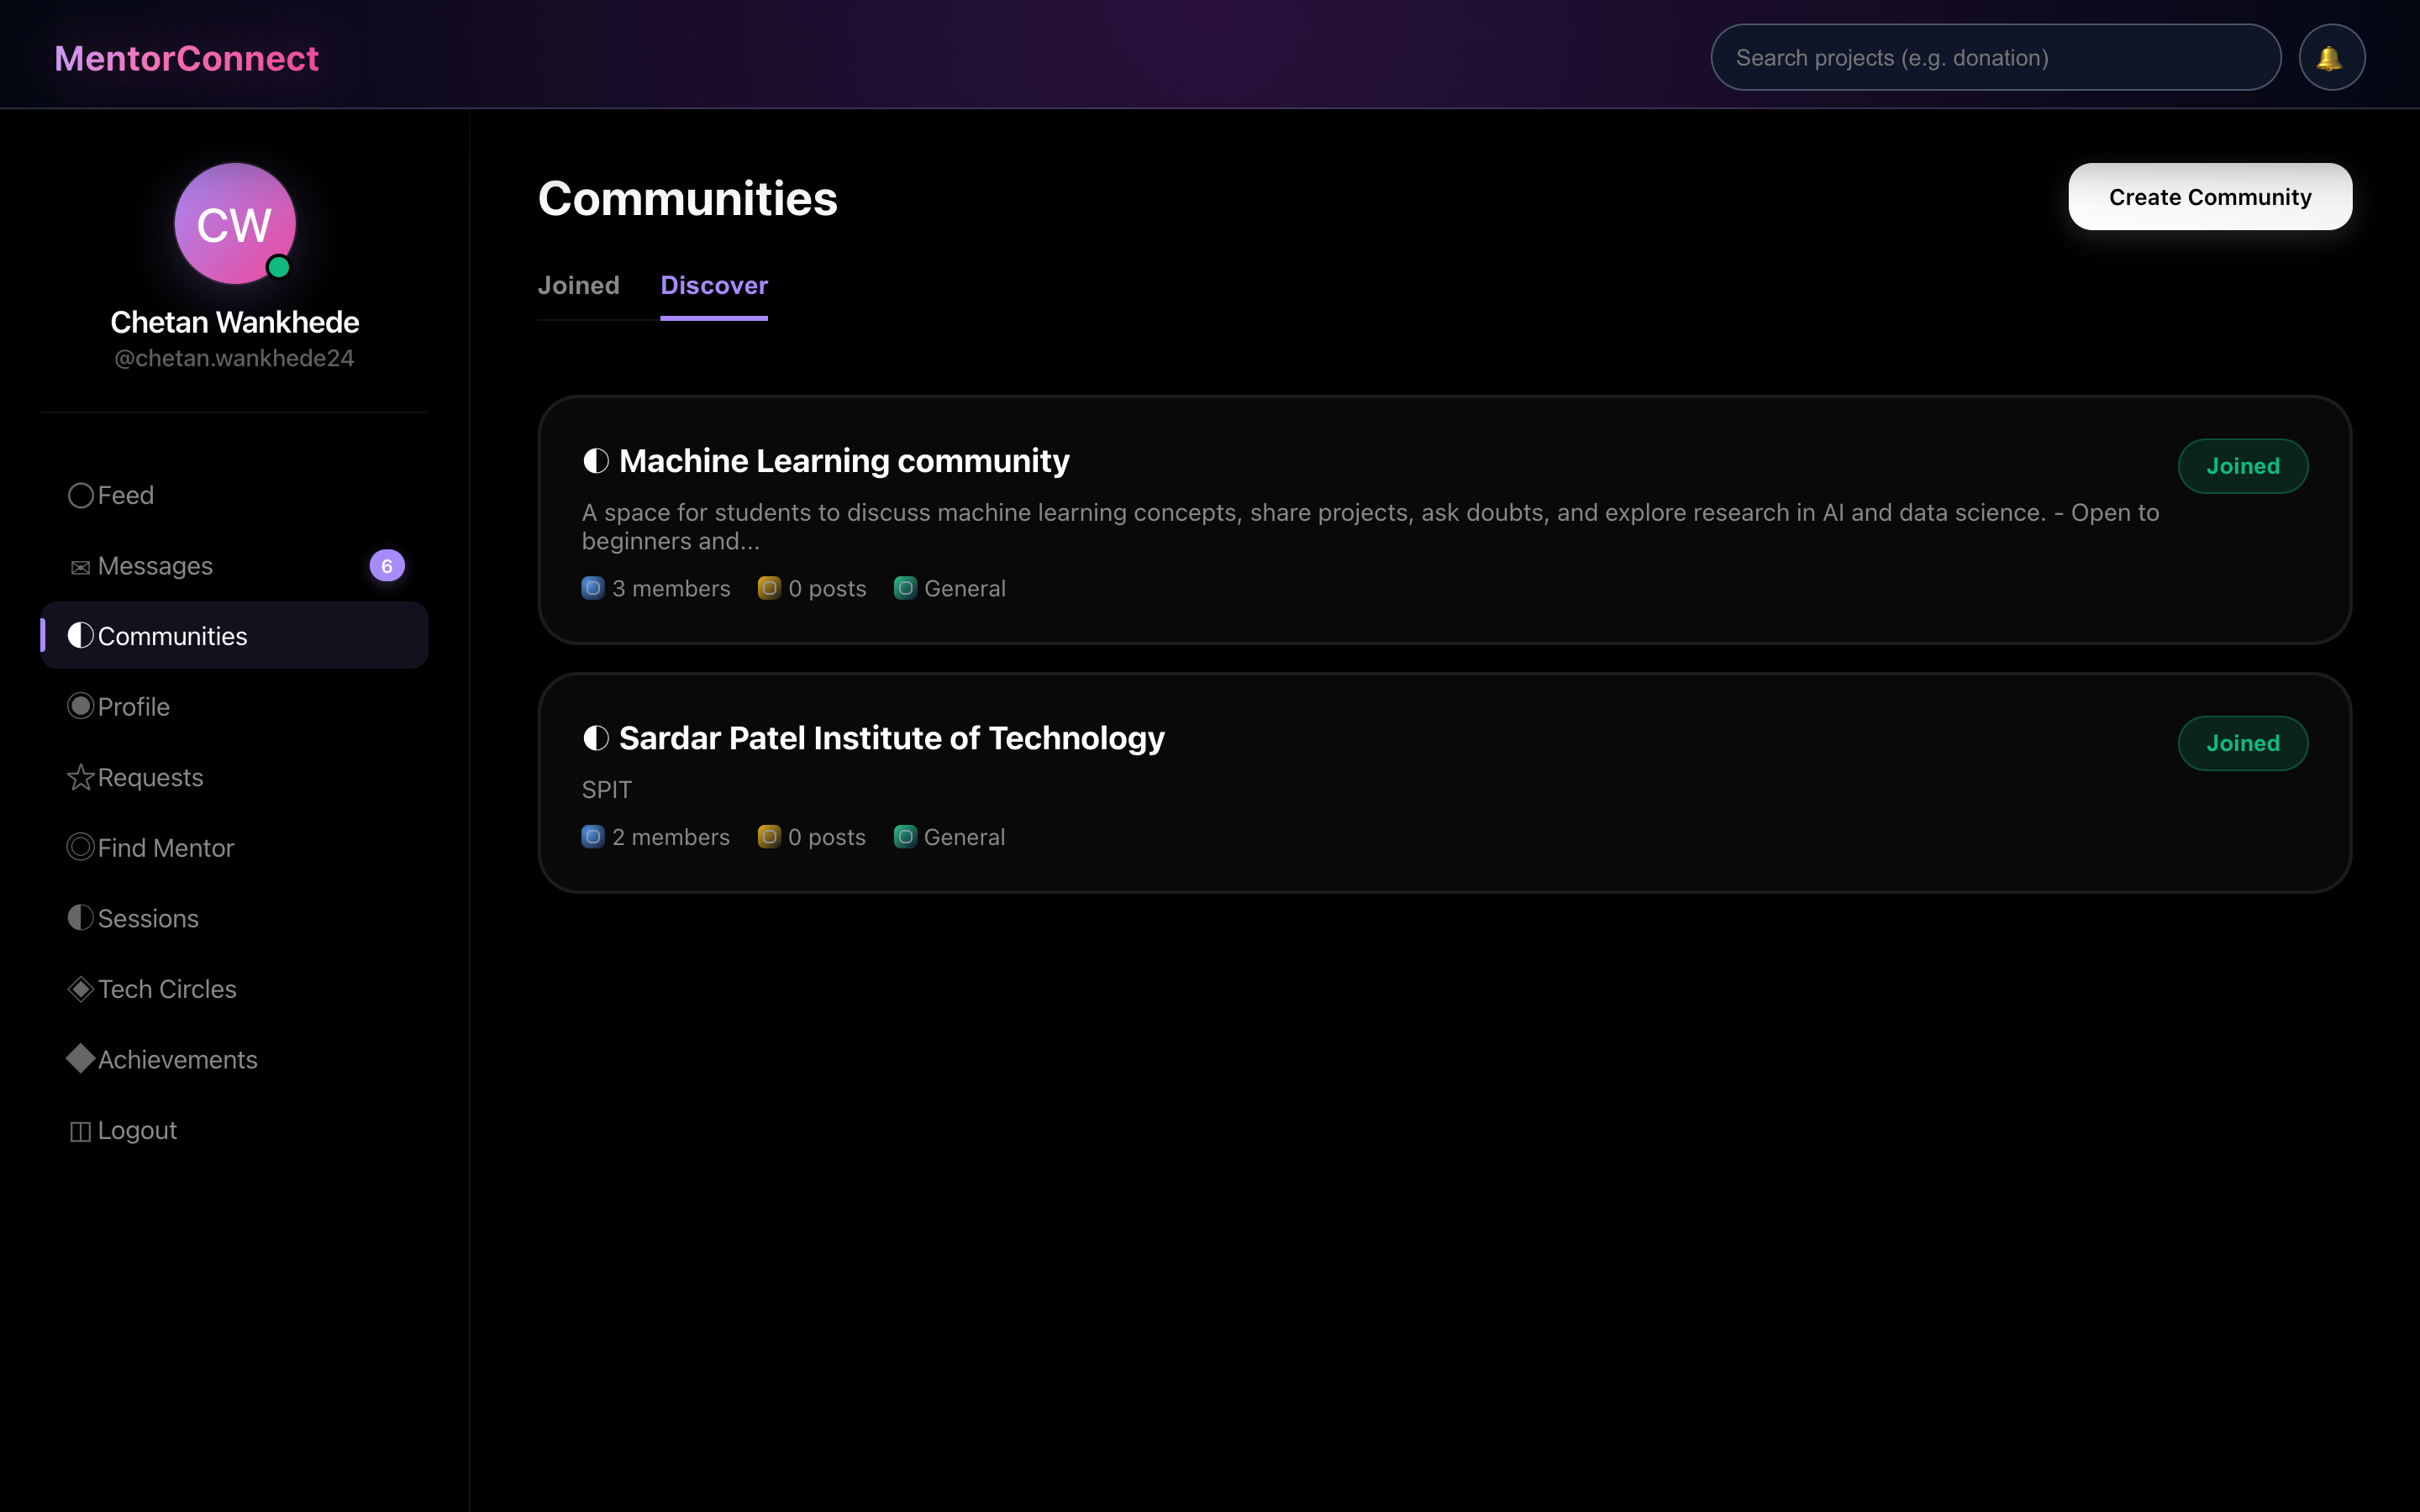
\includegraphics[width=0.95\textwidth]{figures/communities-discover.png}
\caption{Discovering communities with their descriptions, members and categories}
\label{fig:ui-communities-discover}
\end{figure}

\begin{figure}[htbp]
\centering

\includegraphics[width=0.95\textwidth]{figures/community-detail.png}
\caption{A community page with its rules, moderators and posts}
\label{fig:ui-community-detail}
\end{figure}

Students join communities around shared interests (Figures~\ref{fig:ui-communities} and~\ref{fig:ui-communities-discover}). Each community has its own page (Figure~\ref{fig:ui-community-detail}) with a banner, rules, moderators, members and posts, and members can create posts inside it.

\begin{figure}[htbp]
\centering
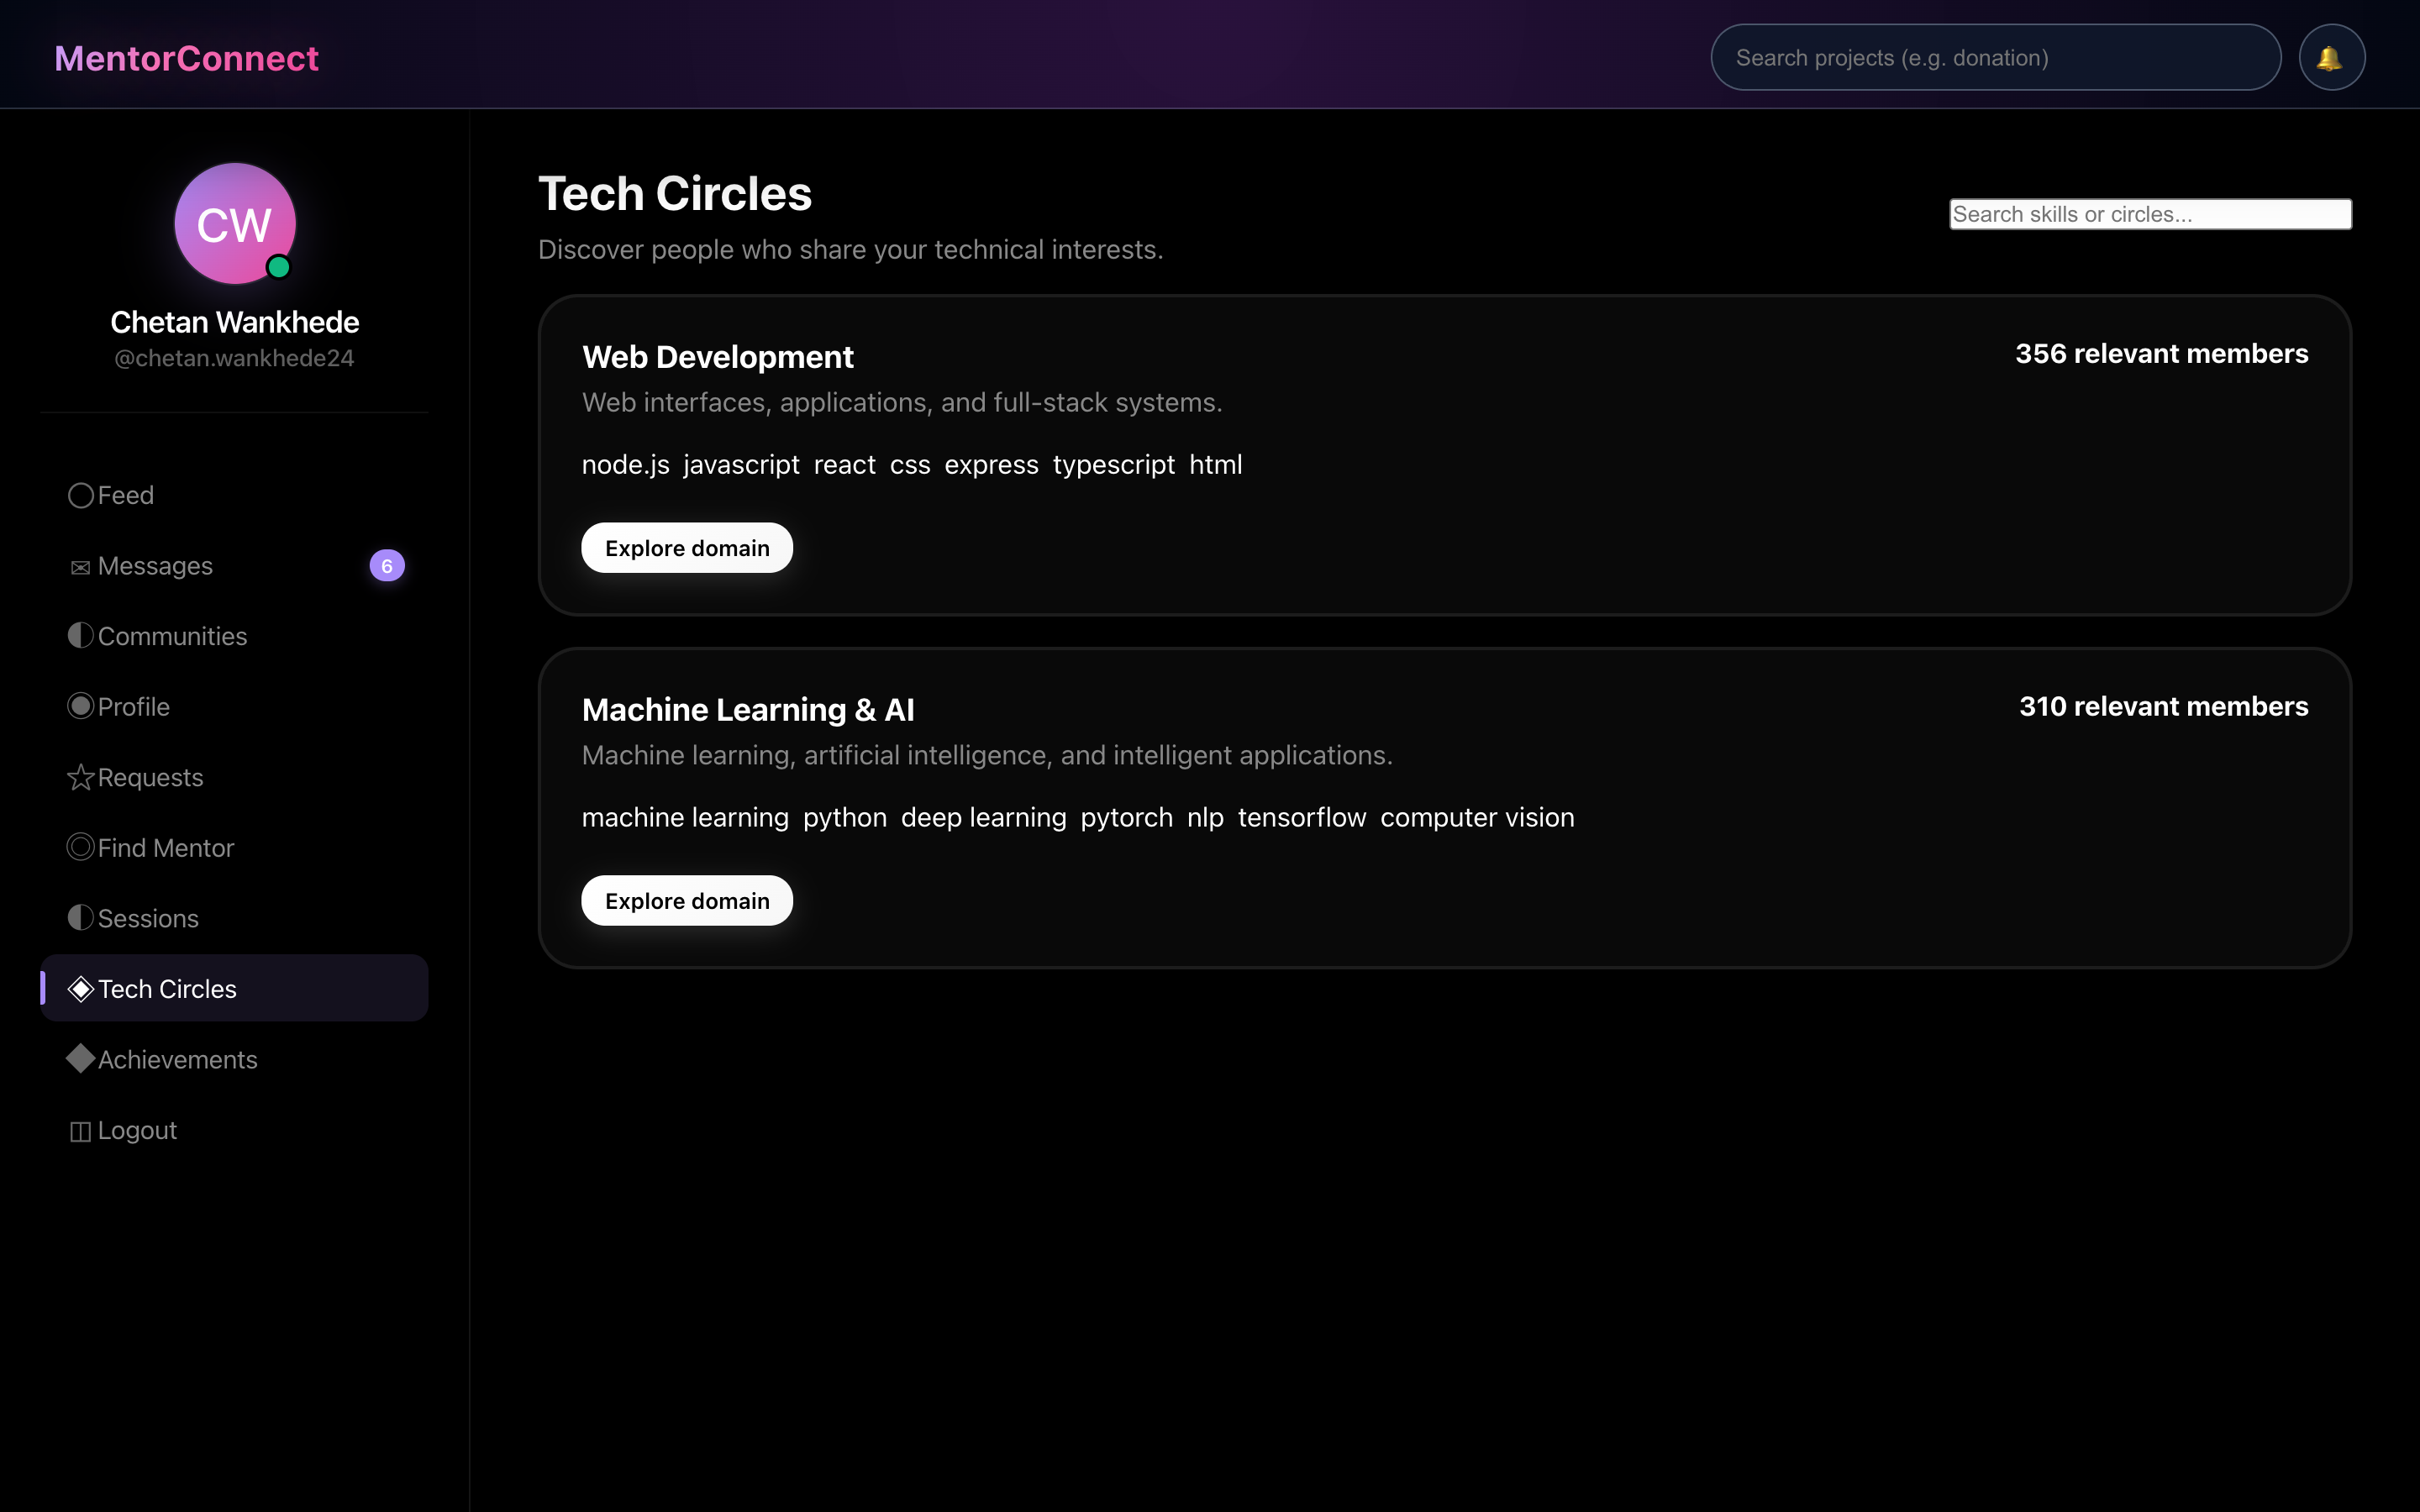
\includegraphics[width=0.95\textwidth]{figures/tech-circles.png}
\caption{Tech Circles: domains formed by clustering students' technical interests}
\label{fig:ui-techcircles}
\end{figure}

\begin{figure}[htbp]
\centering
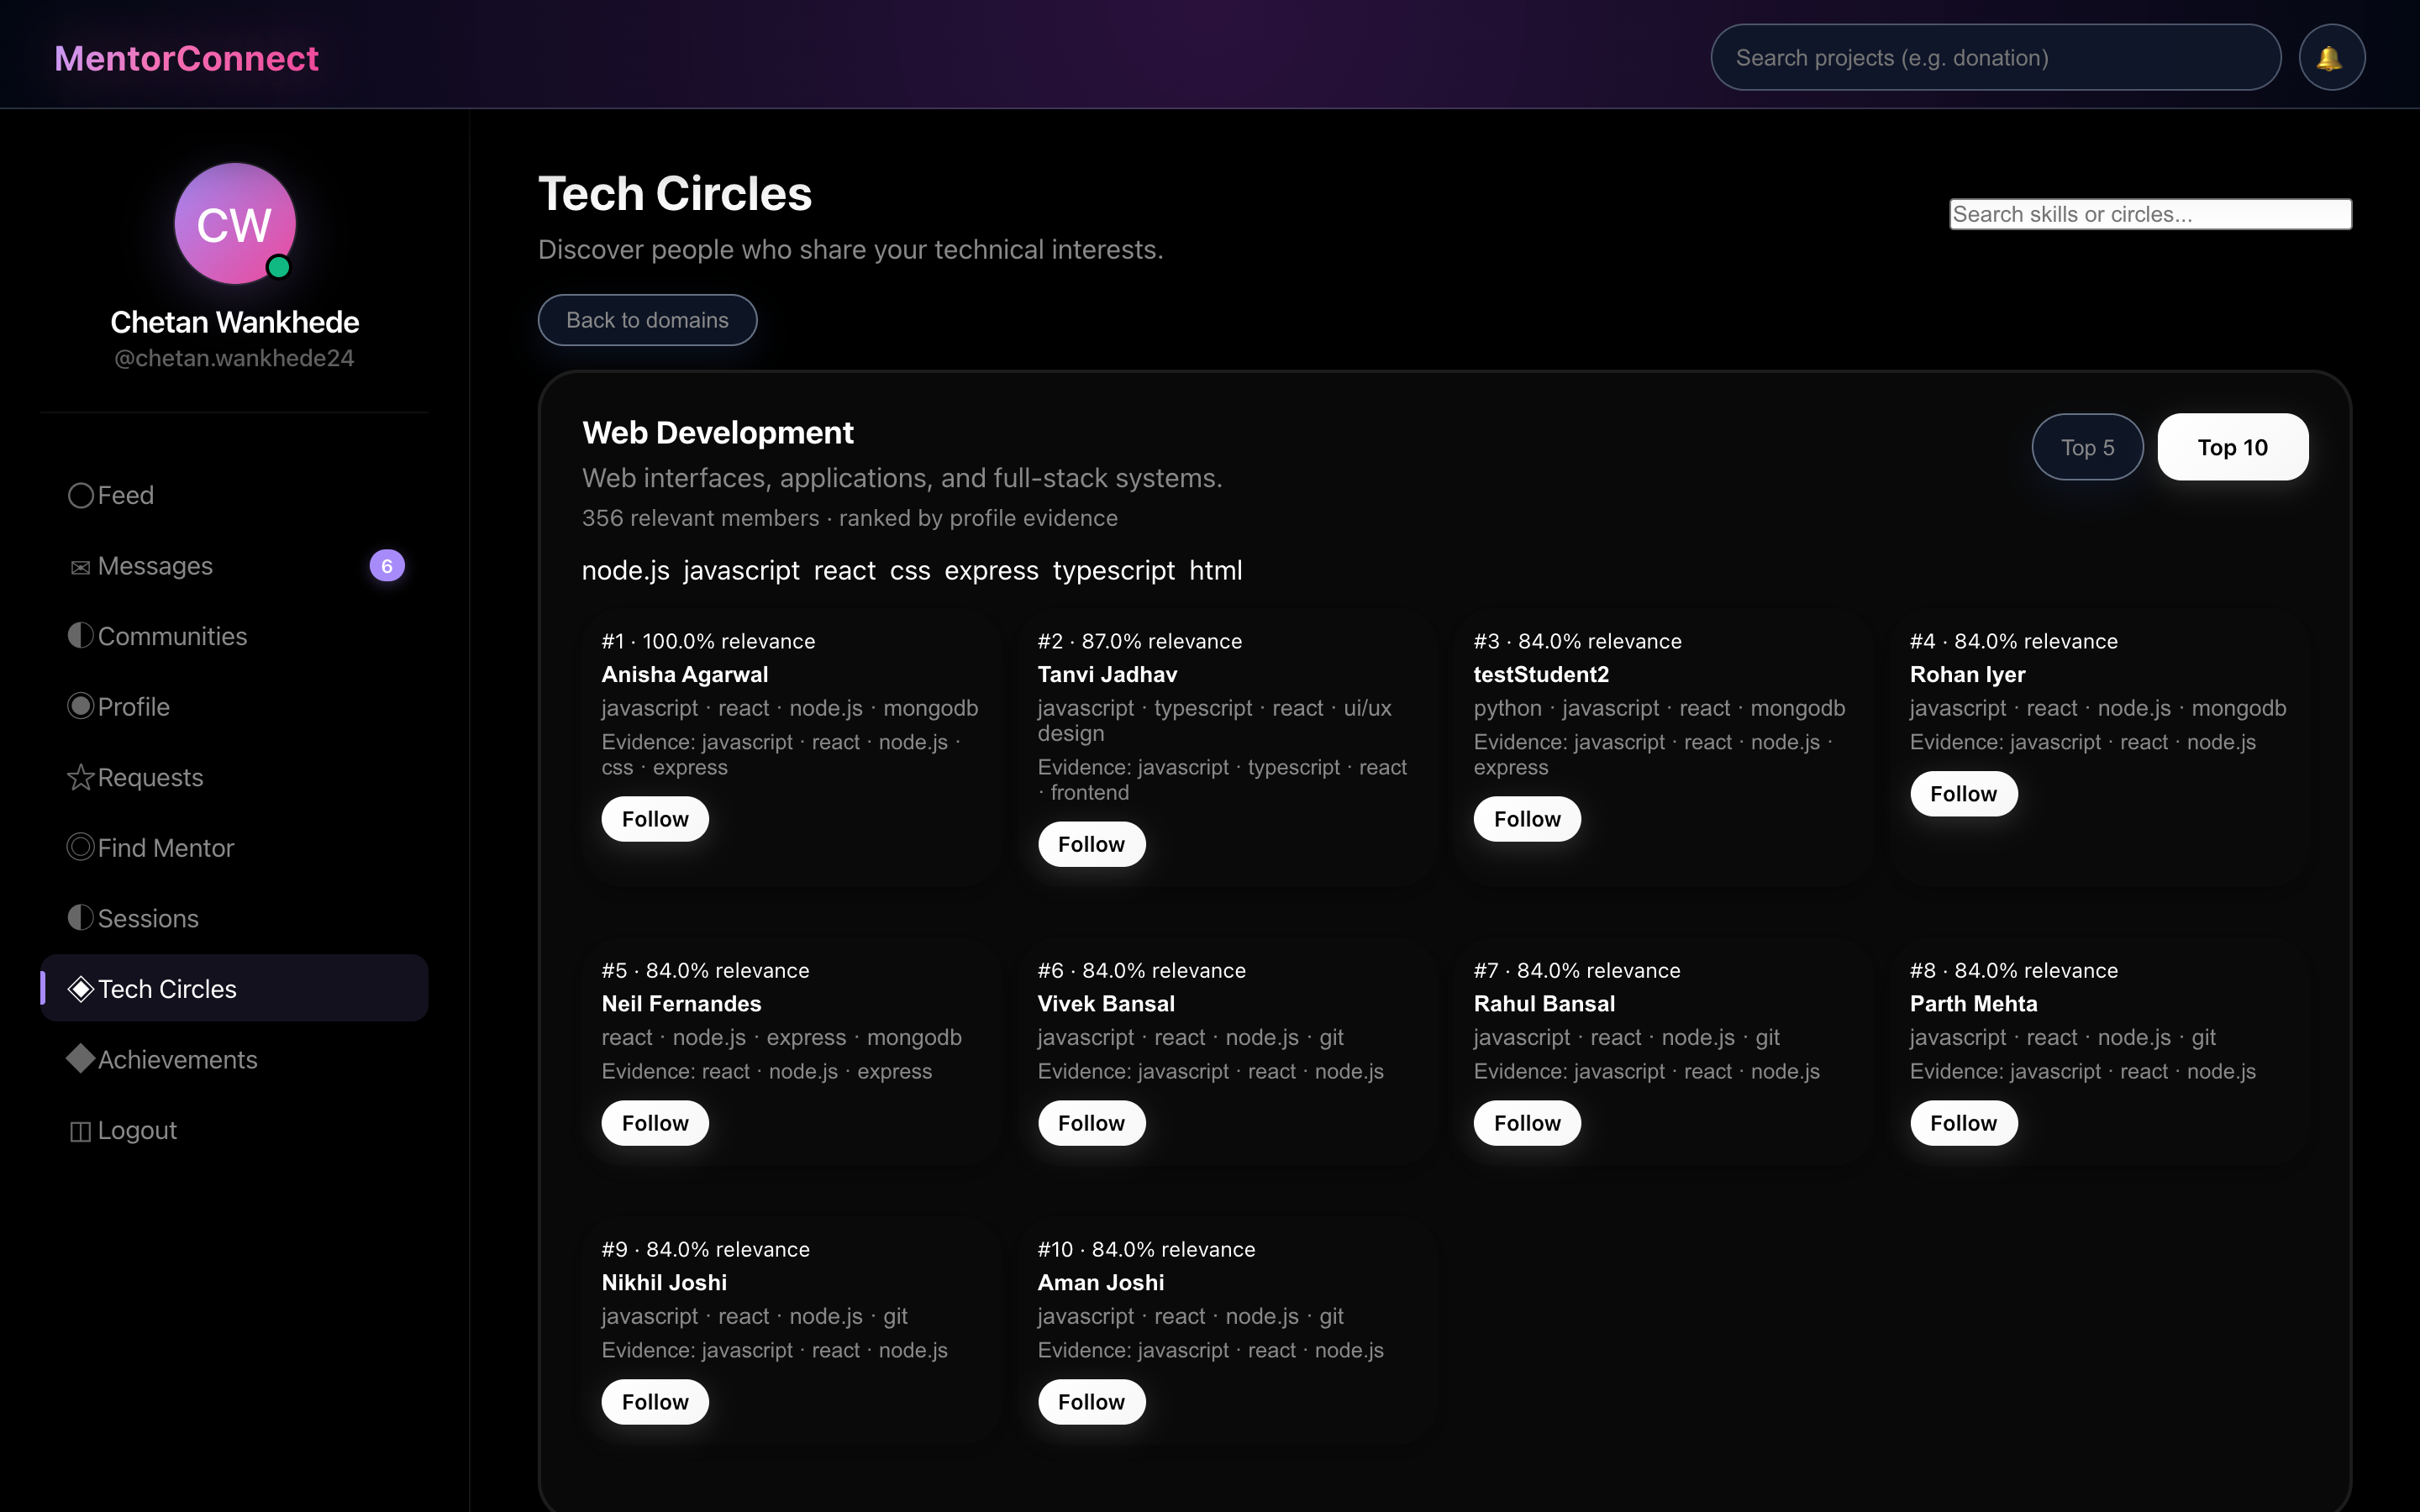
\includegraphics[width=0.95\textwidth]{figures/tech-circle-domain.png}
\caption{A Tech Circle domain listing its most relevant students with the evidence for each}
\label{fig:ui-techcircle-domain}
\end{figure}

Tech Circles (Figure~\ref{fig:ui-techcircles}) groups students into technical domains, such as web development or machine learning, by clustering their skills and interests, and shows the main skills of each domain and the number of relevant members. Exploring a domain (Figure~\ref{fig:ui-techcircle-domain}) ranks its most relevant students with a relevance score and the profile evidence behind it, so students can find and follow peers with shared interests.

\subsection{Sessions, Achievements and Certificates}
\begin{figure}[htbp]
\centering
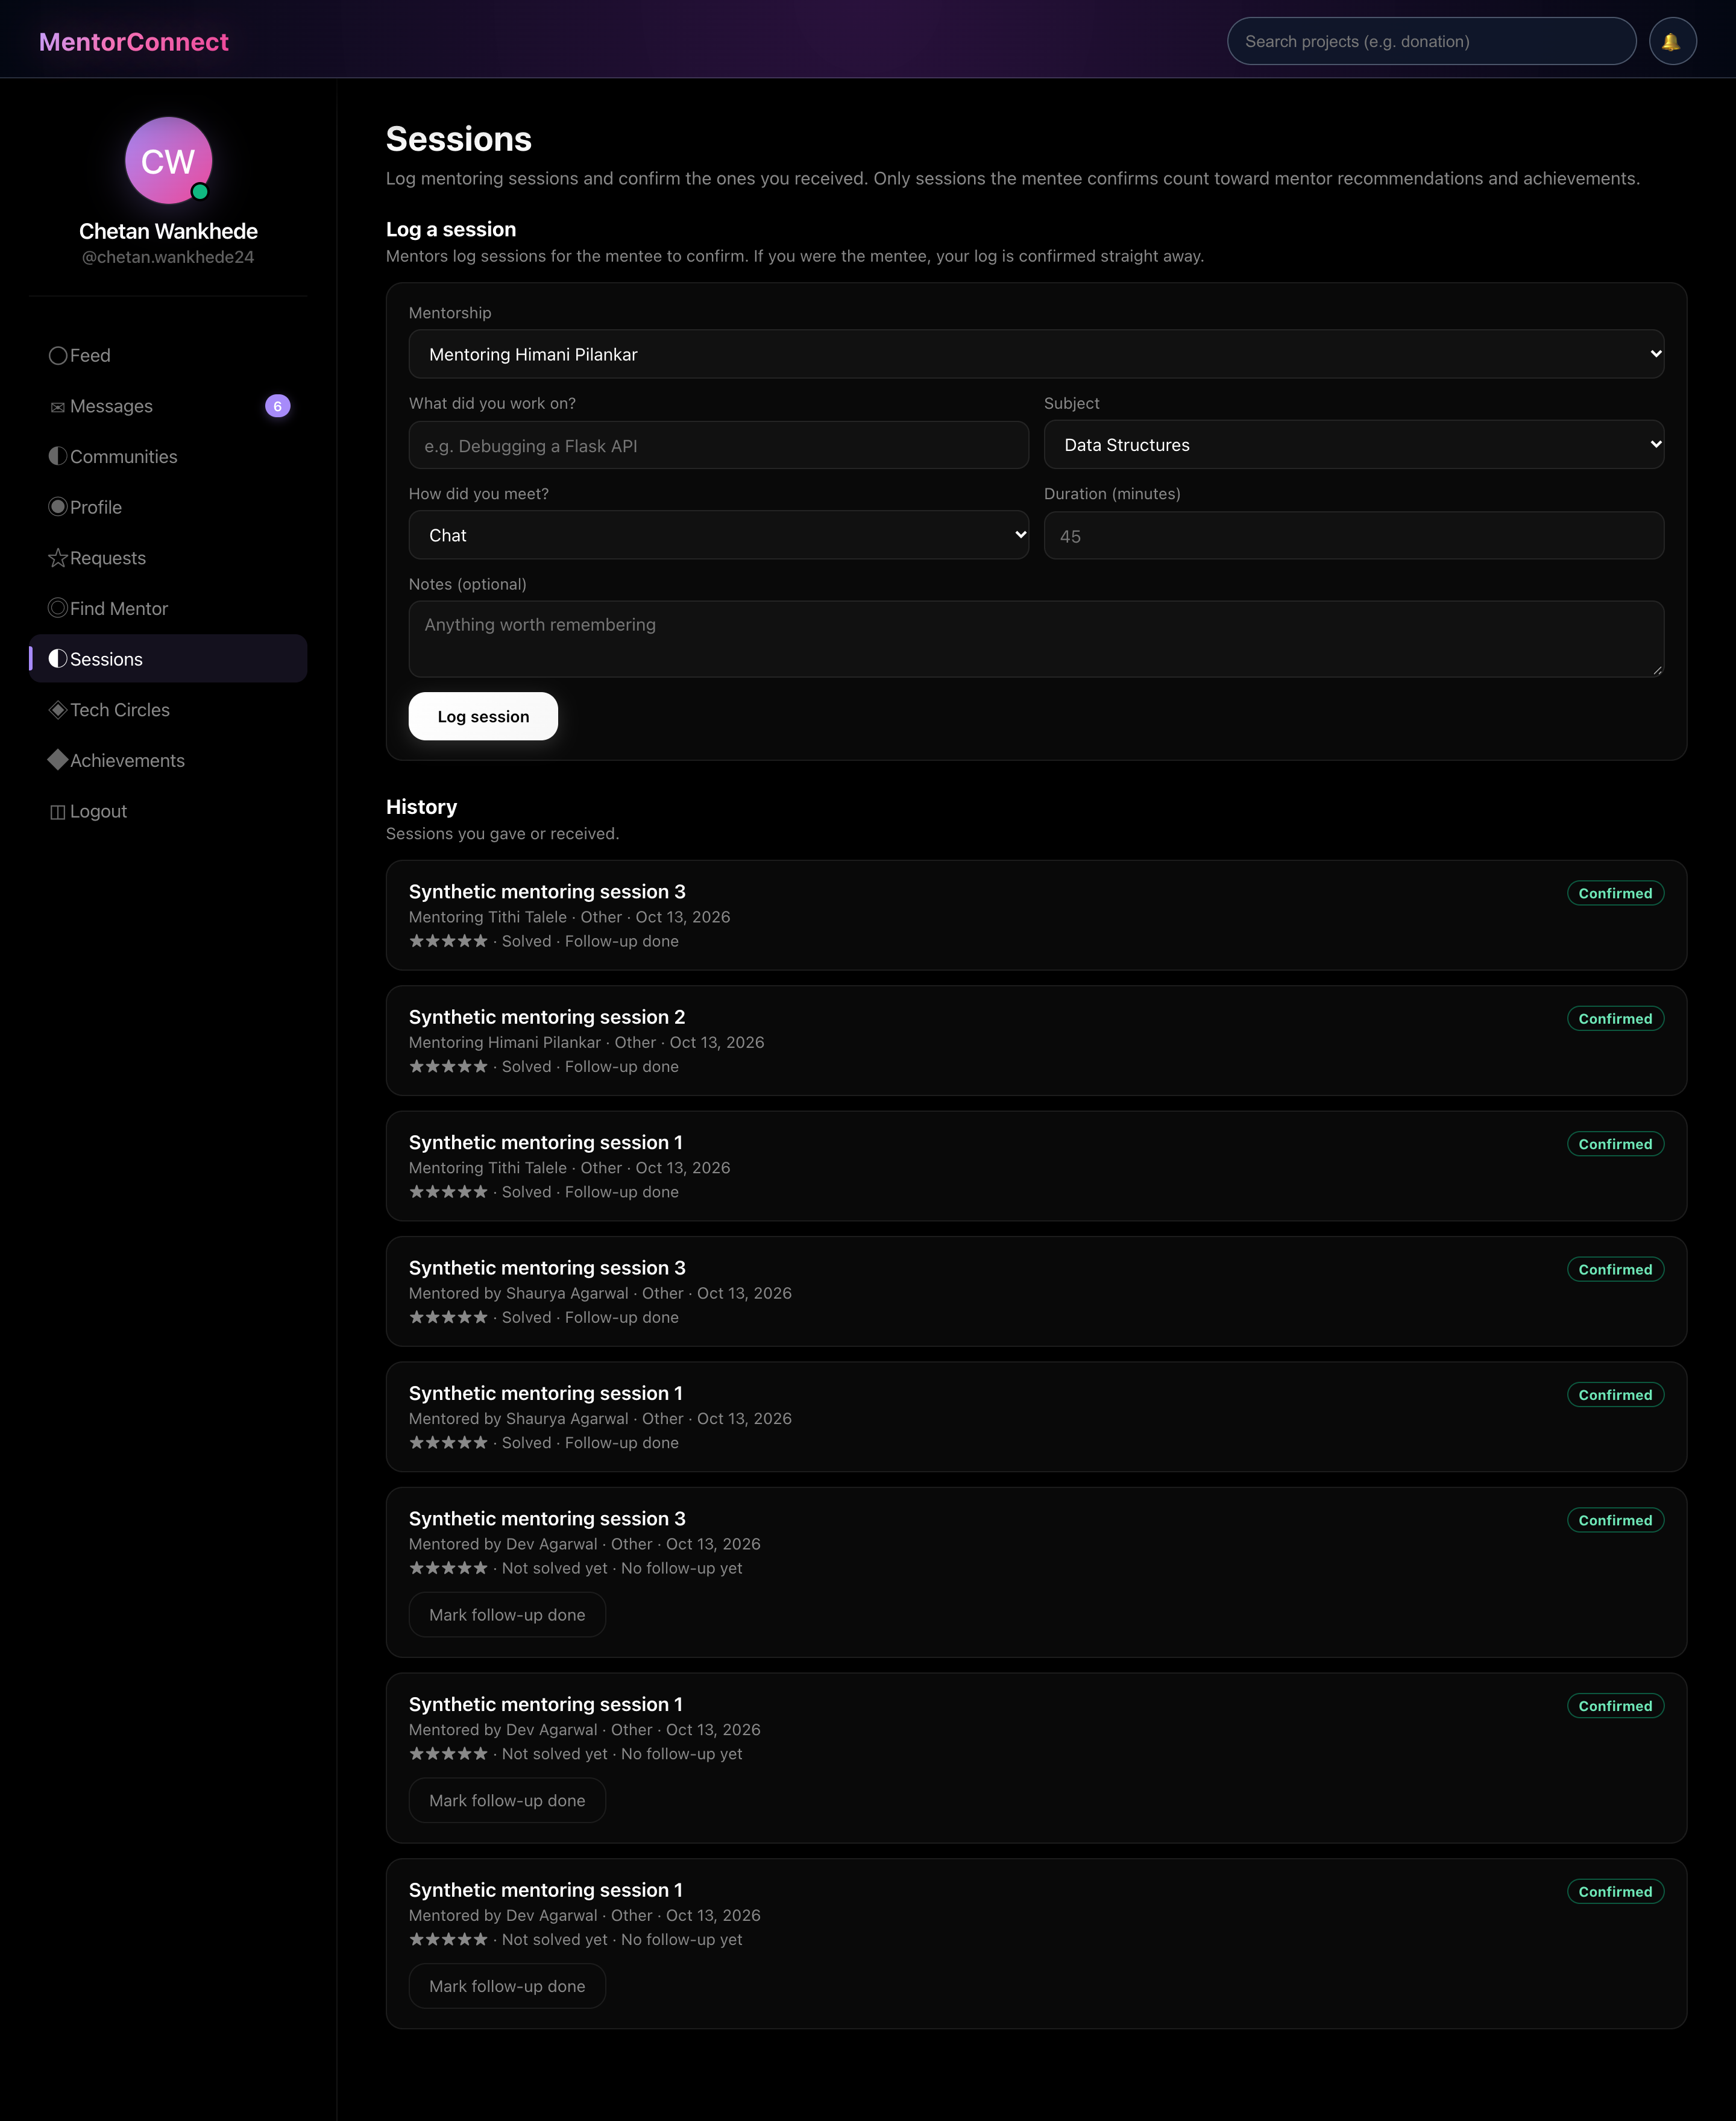
\includegraphics[width=\textwidth,height=0.82\textheight,keepaspectratio]{figures/sessions-full.png}
\caption{Sessions page: logging a session and the history of confirmed sessions}
\label{fig:ui-sessions}
\end{figure}

The Sessions page (Figure~\ref{fig:ui-sessions}) implements the evidence gate described in Section~\ref{sec:gate}. A mentor selects one of their mentorships and logs the topic, subject, meeting type and duration; the mentee then confirms the session and supplies the rating, outcome, follow-up and recommendation, or reports that it did not happen. The history lists every session the student gave or received with its status; confirmed sessions show the mentee's rating, whether the problem was solved and whether the follow-up was completed, and a mentee can mark a follow-up as done later.

\begin{figure}[htbp]
\centering
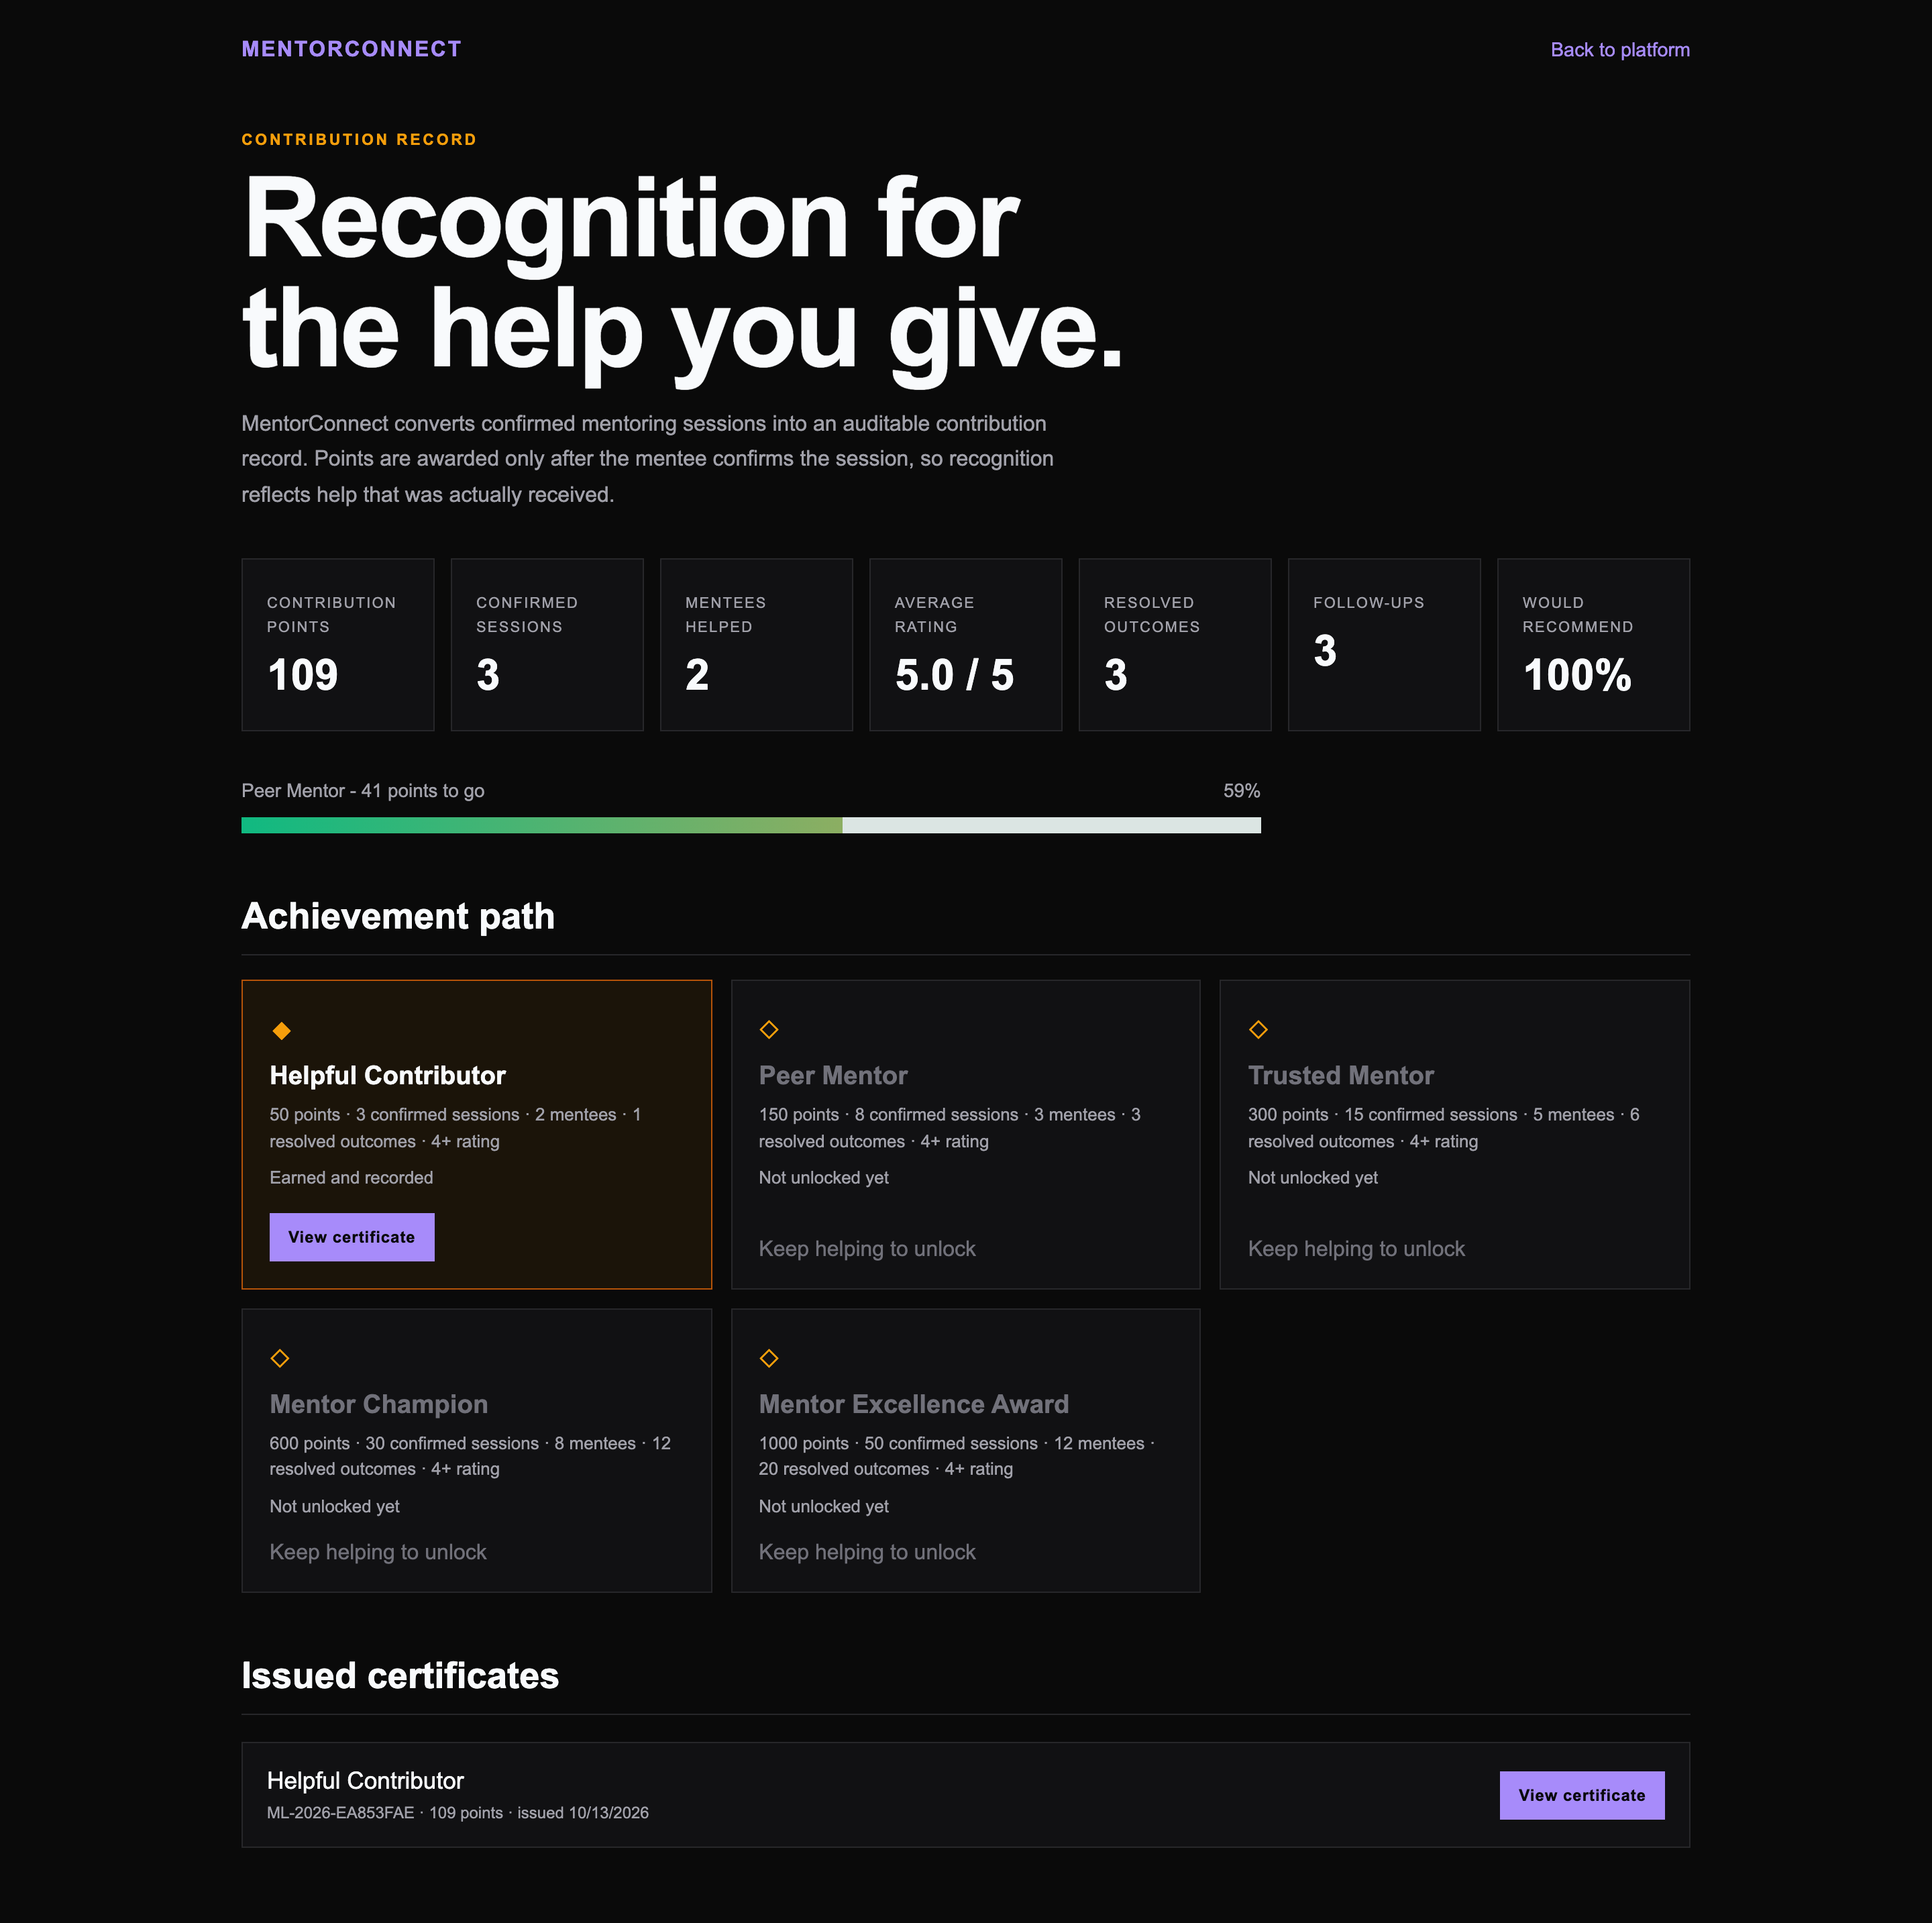
\includegraphics[width=\textwidth,height=0.82\textheight,keepaspectratio]{figures/achievements-full.png}
\caption{Contribution record, achievement path and issued certificates}
\label{fig:ui-achievements}
\end{figure}

\begin{figure}[htbp]
\centering
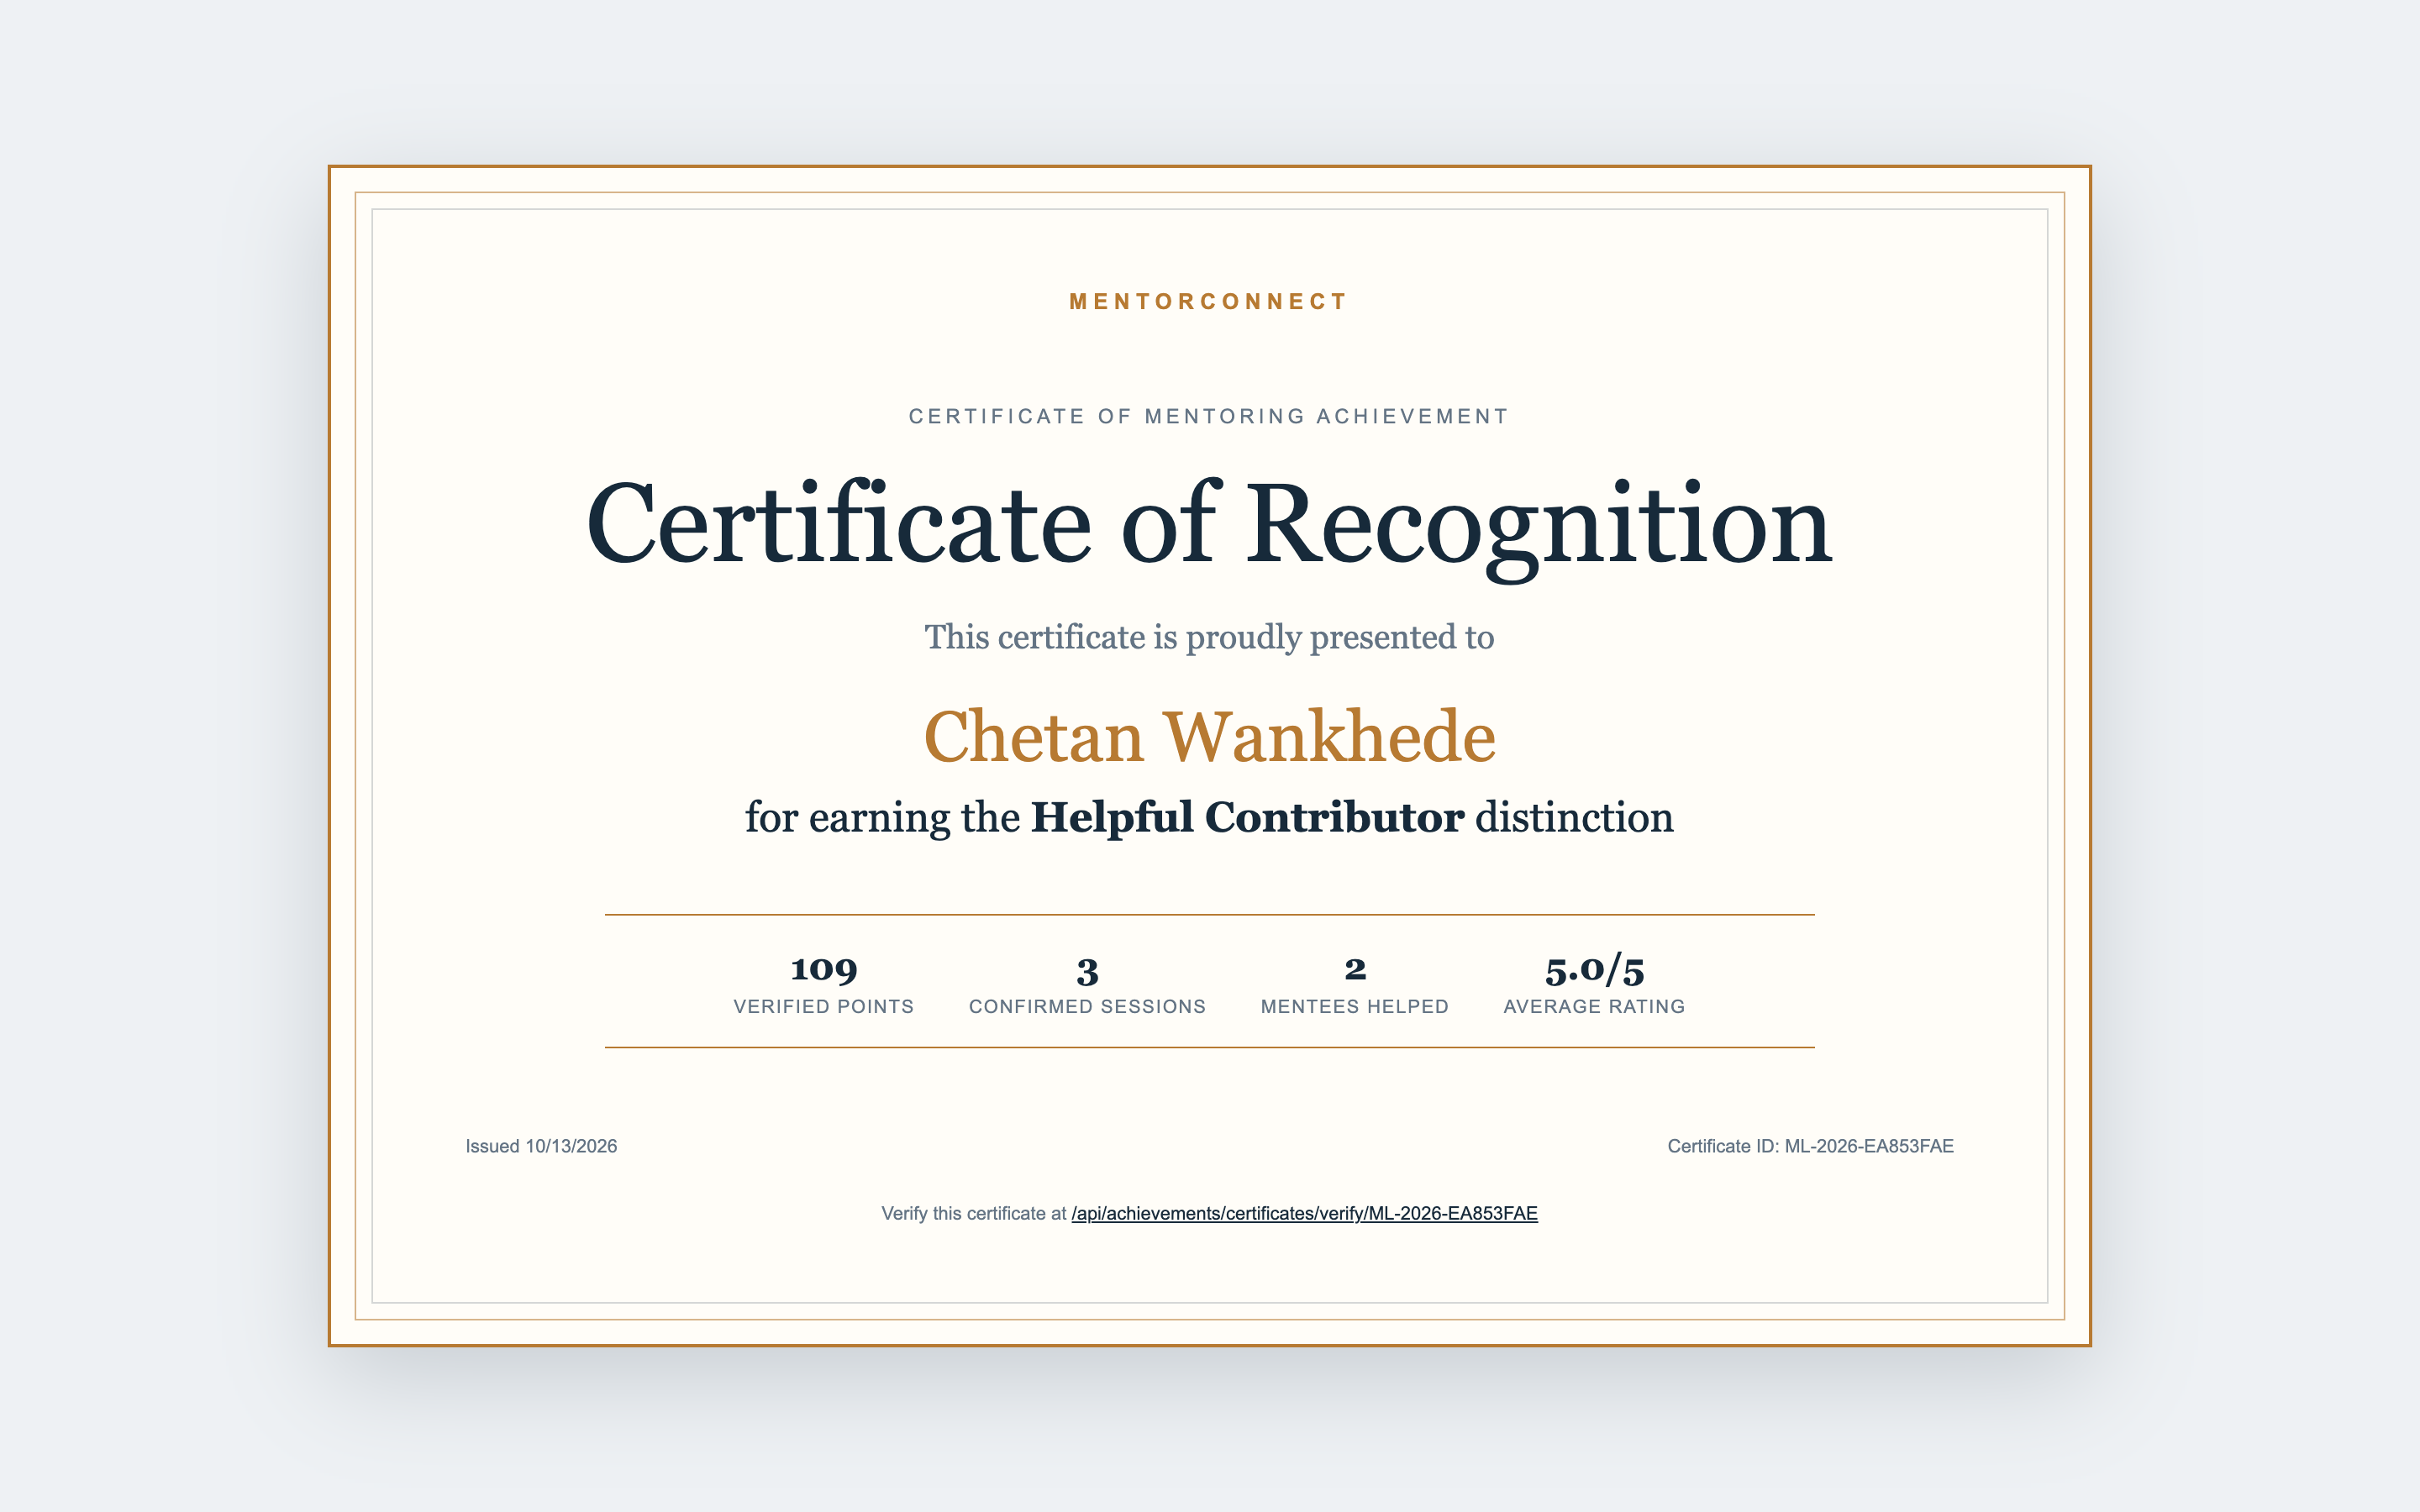
\includegraphics[width=0.95\textwidth]{figures/certificate.png}
\caption{Certificate of Recognition issued for the Helpful Contributor level}
\label{fig:ui-certificate}
\end{figure}

The Achievements page (Figure~\ref{fig:ui-achievements}) shows the mentor's contribution record (contribution points, confirmed sessions, mentees helped, average rating, resolved outcomes, follow-ups and the share of mentees who would recommend them) with progress towards the next level, the full achievement path from Helpful Contributor to Mentor Excellence Award, and the certificates issued so far. Each level requires minimum numbers of sessions, mentees and resolved outcomes and a minimum rating, so it cannot be reached through volume alone. Earned levels produce a formal certificate (Figure~\ref{fig:ui-certificate}) that is emailed to the mentor and can be verified publicly through its certificate ID.

\clearpage
\section{System Verification}
The session tracking and recommendation logging features were verified end to end against an isolated test database, so that no real records were affected. The test suite covers 34 checks, all of which pass. Table~\ref{tab:checks} lists the most important ones. The Python recommendation engine has its own automated unit tests for each engine version, the eligibility rules, the clustering module and model loading.

\begin{table}[h]
\centering
\caption{Key end-to-end verification checks (34 of 34 passed)}
\label{tab:checks}
\small
\begin{tabularx}{\textwidth}{X>{\raggedright\arraybackslash}p{2cm}}
\toprule
\textbf{Check} & \textbf{Result}\\
\midrule
A mentor-logged session starts as pending, and the mentor's own rating is ignored & Passed\\
The mentee is notified and sees the session in their pending list & Passed\\
The mentee can confirm with feedback; confirmed ratings cannot be changed by either party & Passed\\
Only the mentee can mark a follow-up as done, and doing so awards the follow-up points & Passed\\
Only the mentee can dispute a session, and a disputed session cannot be confirmed & Passed\\
A session logged by the mentee is confirmed immediately; invalid ratings are rejected & Passed\\
Sessions confirmed by an external account are stored but earn no points and no ranking credit & Passed\\
Every recommendation list is logged, and confirmed history raises an otherwise identical mentor's score (58\% against 46\%) & Passed\\
The browser cannot fake a request event or write to another user's list & Passed\\
Requests and acceptances are linked back to the list and rank that showed the mentor & Passed\\
\bottomrule
\end{tabularx}
\end{table}

\section{Audit of the Original Engine}
Before designing V3, we audited the original engine (V1) on 448 platform profiles, most of which are synthetic test data, across five random seeds. Table~\ref{tab:audit} summarises the findings. In total, 24 defects were documented in the original engine, including unseeded clustering, weights that exceed one, counting of unconfirmed sessions and the absence of shrinkage for new mentors. These findings motivated the design of V3.

\begin{table}[h]
\centering
\caption{Audit of the original engine (V1)}
\label{tab:audit}
\small
\begin{tabularx}{\textwidth}{>{\raggedright\arraybackslash}p{3.2cm}X}
\toprule
\textbf{Measurement} & \textbf{Finding}\\
\midrule
Tied scores & 87\% of top-10 lists contain tied scores, so part of the order is arbitrary\\
Stability & Average Kendall $\tau$ of 0.71 between runs: rankings change with the random seed\\
Calibration & The highest score observed was 78 out of 100\\
Evidence & Only 11 confirmed sessions existed, so behavioural evidence was sparse\\
\bottomrule
\end{tabularx}
\end{table}

\section{Manipulation Experiment}
\subsection{Setup}
Real mentoring outcomes on the platform are still accumulating, so we evaluated the ranking on simulated campuses with hidden ground truth, which makes it possible to know which mentors are genuinely good and which are gaming the system. Each run contains 150 mentors and 100 students across ten topic areas. Honest mentors have a hidden quality drawn from Beta(5,2) and one to three areas of expertise, and their session volume is only weakly related to their quality. Each session is confirmed by its mentee with probability 0.65, and confirmed sessions carry J-shaped ratings \cite{hu2006}, with outcomes and follow-ups driven by the mentor's quality.

Fifteen percent of mentors are manipulators with low hidden quality, assigned to three strategies: \emph{stuffers} pad their profiles with popular skills and interests; \emph{inflators} self-log many unverified five-star, resolved sessions; and \emph{colluders} have friends confirm fabricated five-star sessions. A mentor is \emph{relevant} to a student if they cover the student's need, are honest, and have a hidden quality of at least 0.65.

Nine rankers were compared: Random; Popularity, which ranks by number of logged sessions; Content-only, which is V3 with no history; V1, where every logged session counts; V3-ungated, which feeds V3 every session as if confirmed, in two forms (as logged, and with honest unconfirmed sessions carrying the feedback the mentee would have given, which is the fair test of the gate); V3 without shrinkage; the evidence-gated V3; and V3 counting at most one session per mentee. V1 and V3 use the platform's ranking code. We report NDCG@10 \cite{jarvelin2002}, Precision@5, mean reciprocal rank (MRR) and the share of top-10 slots taken by manipulators, averaged over 20 random seeds and compared with paired $t$-tests and Wilcoxon tests with Holm correction.

\subsection{Main Results}
\begin{table}[h]
\centering
\caption{Main results at a 15\% manipulator rate (mean over 20 seeds; manipulators form 14.7\% of the pool)}
\label{tab:main}
\small
\begin{tabular}{lcccc}
\toprule
\textbf{Ranker} & \textbf{NDCG@10} & \textbf{P@5} & \textbf{MRR} & \textbf{Manip@10}\\
\midrule
Random & 0.171 & 0.144 & 0.321 & 14.3\%\\
Popularity & 0.118 & 0.051 & 0.154 & 70.5\%\\
Content-only & 0.716 & 0.545 & 0.735 & 18.3\%\\
V1 (all logs) & 0.630 & 0.445 & 0.594 & 32.9\%\\
V3 ungated, as logged & 0.657 & 0.480 & 0.632 & 29.5\%\\
V3 ungated, truthful reports & 0.678 & 0.513 & 0.683 & 26.4\%\\
V3 without shrinkage & 0.724 & 0.615 & 0.791 & 18.0\%\\
\textbf{V3 evidence-gated} & \textbf{0.711} & \textbf{0.585} & \textbf{0.772} & \textbf{19.1\%}\\
\textbf{V3 + one session per mentee} & \textbf{0.723} & \textbf{0.604} & \textbf{0.803} & \textbf{17.2\%}\\
\bottomrule
\end{tabular}
\end{table}

Table~\ref{tab:main} shows that trusting every logged session is harmful. V1 performs worse than ignoring history altogether: its NDCG@10 falls to 0.630 against 0.716 for Content-only, and manipulators take 32.9\% of top-10 slots, more than twice their share of the pool. Popularity, the extreme case of trusting activity, gives 70.5\% of the top 10 to manipulators.

The two V3-ungated rows use the same ranking model as V3 and differ only in whether unconfirmed sessions count, so comparing them with V3 isolates the gate. Even against the fair version, in which honest unconfirmed sessions carry truthful feedback, the gate raises NDCG@10 by 0.033, Precision@5 by 0.071 and MRR by 0.089, and lowers the manipulator share from 26.4\% to 19.1\%. V3 is better on every accuracy metric in each of the 20 runs ($p<0.001$). Compared with V1, manipulator exposure falls by 42\%. Compared with Content-only, verified history raises Precision@5 by 7\% and MRR by 0.037, while manipulator exposure stays within 2.5 percentage points. Removing shrinkage leaves robustness unchanged, which shows that the protection comes from the gate itself; shrinkage gives mentors with little history a fairer chance.

\begin{table}[h]
\centering
\caption{Share of top-10 slots by manipulation strategy (stuffers 5.3\%, inflators 4.7\% and colluders 4.7\% of the pool)}
\label{tab:attack}
\small
\begin{tabular}{lccc}
\toprule
\textbf{Ranker} & \textbf{Stuffer} & \textbf{Inflator} & \textbf{Colluder}\\
\midrule
Random & 5.3\% & 4.6\% & 4.4\%\\
Content-only & 9.2\% & 4.6\% & 4.5\%\\
V1 (all logs) & 6.4\% & 16.8\% & 9.8\%\\
V3 ungated, truthful reports & 5.0\% & 13.4\% & 8.0\%\\
\textbf{V3 evidence-gated} & 6.0\% & \textbf{3.1\%} & 9.9\%\\
\textbf{V3 + one session per mentee} & 6.2\% & 3.3\% & \textbf{7.7\%}\\
\bottomrule
\end{tabular}
\end{table}

Table~\ref{tab:attack} breaks the results down by strategy. Inflators are the main threat to V1, where they hold 16.8\% of the top 10; under the gate they fall to 3.1\%, below even the Random ranker. Verified history also dilutes profile stuffing, from 9.2\% under Content-only to 6.0\%. Colluders, whose friends confirm fabricated sessions, are limited by counting at most one session per mentee, which lowers their share from 9.9\% to 7.7\%. Under the strongest collusion tested, with ten friends and 20--40 fabricated sessions each, the same rule cuts their share from 14.7\% to 10.7\% and raises NDCG@10 from 0.679 to 0.707.

\subsection{Robustness as Manipulation Grows}
\begin{figure}[h]
\centering
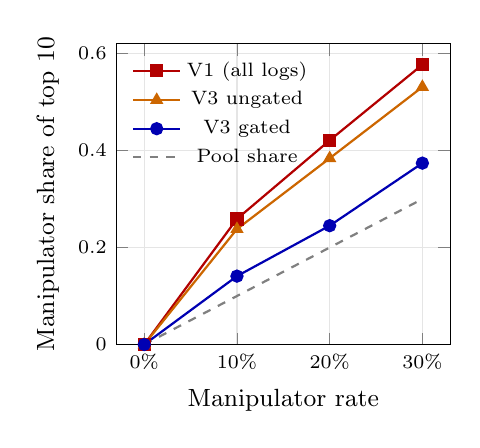
\begin{tikzpicture}
\begin{axis}[width=0.48\textwidth, height=5.4cm, xlabel={Manipulator rate}, ylabel={Manipulator share of top 10},
  xtick={0,0.1,0.2,0.3}, xticklabels={0\%,10\%,20\%,30\%}, ymin=0, ymax=0.62,
  legend style={font=\scriptsize, at={(0.02,0.98)}, anchor=north west, draw=none, fill=none},
  tick label style={font=\scriptsize}, label style={font=\small}, grid=major, grid style={gray!20}]
\addplot[mark=square*, red!70!black, thick] coordinates {(0,0) (0.1,0.259) (0.2,0.421) (0.3,0.577)};
\addlegendentry{V1 (all logs)}
\addplot[mark=triangle*, orange!80!black, thick] coordinates {(0,0) (0.1,0.238) (0.2,0.384) (0.3,0.531)};
\addlegendentry{V3 ungated}
\addplot[mark=*, blue!70!black, thick] coordinates {(0,0) (0.1,0.141) (0.2,0.245) (0.3,0.374)};
\addlegendentry{V3 gated}
\addplot[dashed, gray, thick] coordinates {(0,0) (0.3,0.3)};
\addlegendentry{Pool share}
\end{axis}
\end{tikzpicture}\hfill
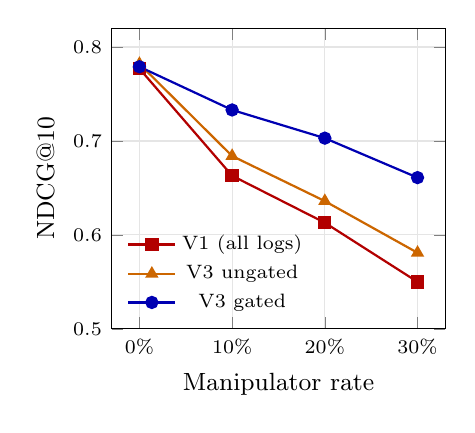
\begin{tikzpicture}
\begin{axis}[width=0.48\textwidth, height=5.4cm, xlabel={Manipulator rate}, ylabel={NDCG@10},
  xtick={0,0.1,0.2,0.3}, xticklabels={0\%,10\%,20\%,30\%}, ymin=0.5, ymax=0.82,
  legend style={font=\scriptsize, at={(0.02,0.02)}, anchor=south west, draw=none, fill=none},
  tick label style={font=\scriptsize}, label style={font=\small}, grid=major, grid style={gray!20}]
\addplot[mark=square*, red!70!black, thick] coordinates {(0,0.777) (0.1,0.663) (0.2,0.613) (0.3,0.550)};
\addlegendentry{V1 (all logs)}
\addplot[mark=triangle*, orange!80!black, thick] coordinates {(0,0.782) (0.1,0.684) (0.2,0.636) (0.3,0.581)};
\addlegendentry{V3 ungated}
\addplot[mark=*, blue!70!black, thick] coordinates {(0,0.779) (0.1,0.733) (0.2,0.703) (0.3,0.661)};
\addlegendentry{V3 gated}
\end{axis}
\end{tikzpicture}
\caption{Manipulator exposure (left) and ranking accuracy (right) as the share of manipulators grows}
\label{fig:sweep}
\end{figure}

Figure~\ref{fig:sweep} varies the share of manipulators from 0\% to 30\%. V1 over-exposes manipulators at every level, giving them 57.7\% of the top 10 when they make up 30\% of mentors, and its NDCG@10 falls from 0.777 to 0.550. The evidence-gated V3 keeps the manipulator share close to their share of the pool and retains far more accuracy (0.661 at 30\%). With no manipulators, all rankers score within 0.011 NDCG@10 of each other, so the gate costs nothing on an honest campus.

\subsection{When Verified History Pays Off}
\begin{table}[h]
\centering
\caption{Mature campus with four times more session history (mean over ten seeds)}
\label{tab:mature}
\small
\begin{tabular}{lcccc}
\toprule
\textbf{Ranker} & \textbf{NDCG@10} & \textbf{P@5} & \textbf{MRR} & \textbf{Manip@10}\\
\midrule
Content-only & 0.716 & 0.550 & 0.746 & 18.2\%\\
V1 (all logs) & 0.685 & 0.543 & 0.721 & 24.3\%\\
V3 ungated, truthful reports & 0.718 & 0.605 & 0.790 & 19.7\%\\
\textbf{V3 evidence-gated} & \textbf{0.735} & \textbf{0.643} & \textbf{0.825} & \textbf{16.1\%}\\
\textbf{V3 + one session per mentee} & \textbf{0.738} & \textbf{0.648} & \textbf{0.832} & \textbf{15.3\%}\\
\bottomrule
\end{tabular}
\end{table}

The value of verified history grows as it accumulates. Table~\ref{tab:mature} repeats the experiment with four times as much history. The evidence-gated V3 now beats Content-only on every accuracy metric, with Precision@5 of 0.643 against 0.550 (an improvement of 17\%), and also gives manipulators fewer top-10 slots (16.1\% against 18.2\%). Counting one session per mentee improves the results slightly further.

\section{Discussion}
The results support a simple design rule for platforms that rank people: let the counter-party write the evidence. Controlling who may create a record is a stronger defence than detecting manipulation after the fact, needs no examples of past attacks, and costs nothing when nobody is cheating. Requiring that the counter-party be a verified member of the institute closes the route of creating outside accounts, and counting each mentee at most once limits what a group of colluding friends can achieve. Because every recommendation list is logged, a campus pilot can measure request and acceptance rates directly and confirm these findings with real use.

%======================== CHAPTER 5 ========================
\chapter{Conclusion and Future Work}
MentorConnect turns informal peer mentoring into a verified, structured and measurable process. Students can sign up with their institute email, build academic profiles, discover mentors through an explainable recommendation engine, request and manage mentorships, chat in real time and take part in communities. Mentors are recognised through auditable points, achievement levels and publicly verifiable certificates, and the institute gains analytics-ready records of mentoring activity.

The central contribution of the project is evidence gating: a mentor's history influences their ranking and recognition only through sessions that a verified student mentee confirmed and supplied feedback for. Our audit of the original engine found 24 defects, including arbitrary tie-breaking, unstable rankings and the counting of unconfirmed activity. In a controlled experiment over 20 random campuses using the platform's ranking code, trusting every logged session lowered NDCG@10 by 12\% and gave manipulators more than twice their share of top-10 slots. The evidence-gated engine reversed this in every run, reduced manipulator exposure by 42\% compared with the original engine, pushed self-logged inflation below random-chance exposure, and improved top-5 precision over a content-only ranker by 7\%, rising to 17\% as verified history accumulated. Counting each mentee at most once further limited collusion while improving accuracy.

Several directions remain for future work. A campus pilot at the institute would use the recommendation logs to measure request rates, acceptance rates and session ratings from real use. Exposure-aware re-ranking would spread students evenly across mentors and give new mentors more visibility. The experimental learned ranker (V4) can be trained on logged outcomes once enough data exists and compared with V3. Skill verification through endorsements or project evidence would further strengthen mentor profiles. A mobile application, institute single sign-on and a broader automated test suite would make the platform ready for wider deployment.

%======================== CHAPTER 6 ========================
\chapter{Publication}
\section{Who Writes the Evidence? Counterparty-Confirmed Track Records in MentorConnect}
A research paper describing the evidence-gating approach and the manipulation experiment has been prepared from this work by Himani Pilankar, Tithi Talele, Chetan Wankhede and Dr.\ Sudhir Dhage for submission to a peer-reviewed IEEE conference. The paper states evidence gating as a set of enforceable rules for people-ranking platforms, describes its implementation in MentorConnect, and reports the results presented in Chapter~4: across 20 random campuses, the evidence gate improves accuracy and reduces manipulator exposure in every run, neutralises self-logged inflation, and, with one session counted per mentee, limits collusion while delivering the best accuracy of all rankers tested.

\bibliographystyle{IEEEtran}
\bibliography{references}

\end{document}
